\begin{SingleSpace}
\chapter{Wave-Mean Flow Interactions in Tidally Locked Atmospheres}\label{ch:wave-mean-flow}
% \vspace{0.5cm}
% \chapterprecishere{``I scarcely need remark that I look upon Laplace's process as a mere sport with symbols, and upon Laplace's conclusion as a grievous error.''\par\raggedleft--- \textupGeorge Biddell Airy}
% \chapterprecishere{``One might as well approximate the derivatives well instead of badly''\par\raggedleft--- \textup{John P. Boyd}, Chebyshev and Fourier Spectral Methods}
\end{SingleSpace}
% \vspace{0.5cm}

\noindent
 \vspace*{-0.5cm}
\textit{Most of the results in this chapter are published in \citet{hammond2018wavemean}.}
 \vspace*{0.5cm}

%0 -- LEAD-IN PARAGRAPHS

%START ELEMENT
% Tidally locked planetary atmospheres have such a different spatial energy input to planets like the Earth that it is not obvious that conventional Earth-like atmospheric dynamics should be able to describe them. However, the planetary-scale day-night forcing difference makes the global circulation highly susceptible to a simple shallow-water model, compared to the higher order effects controlling the Earth's atmosphere.

Strong zonal eastward jets are seen in simulations of tidally locked planetary atmospheres, and their effects on the temperature distribution in the atmosphere have been observed on many planets \citep{parmentier2017handbook}. This chapter shows how a shallow-water model linearised around a zonal jet $\overline{U}(y)$ reproduces the global circulation of simulated tidally locked planets. This zonal flow creates their distinctive global circulation pattern, and controls their temperature distribution. I will show that the eastward hot-spot shift, which has been observed on many planets, is due to a Doppler-shift of the stationary waves excited by the day-night forcing difference \citep{tsai2014three}.

%SIGNPOSTS
Sections \ref{sec:shallow-water} and \ref{sec:shear-flow-beta-plane} will show how the zonal flow discussed in Chapter \ref{ch:eqm-zonal-flow} affects the free and forced modes in the linear shallow-water model of \citet{showman2011superrotation}. In Section \ref{sec:shear-flow-beta-plane}, I will linearise the shallow-water model about a shear zonal flow $\overline{U}(y)$ and its associated geostrophic height perturbation $\overline{H}(y)$. This differs from \citet{showman2011superrotation}, who used zero background flow $\overline{U}(y)=0$ and a uniform background height $\overline{H}(y) = H_{0}$. It also differs from \citet{tsai2014three}, who used a uniform background flow $\overline{U}(y)=U_{0}$ and a uniform background height $\overline{H}(y) = H_{0}$.  Chapter \ref{ch:eqm-zonal-flow} justifies the eastward flow $\overline{U}(y)$ imposed at all latitudes, which would otherwise contradict the predicted acceleration in \citet{showman2011superrotation}.

 In Section \ref{sec:shear-flow-sphere}, I will construct the same linear model on a sphere rather than on a beta-plane, for direct comparison with GCM simulations and real planets. I will then use this model to predict how the observable features of the global circulation qualitatively scale with different planetary parameters. Finally, I will discuss the mechanism behind the observable ``hot-spot shift'' on tidally locked planets. I will conclude that the shallow-water model linearised about the jet $\overline{U}(y)$ and its height perturbation $\overline{H}(y)$, matches the results of GCM simulations and explains the form of the global circulation and temperature distribution.


%%%%%%%%%%%%%%%%%%%%%%%%%%%%%%%%%%%%
%SECTION 1 -- LINEAR SHALLOW-WATER AND UNIFORM FLOW
\section{Linear Shallow-Water Model in Zonal Flow}\label{sec:shallow-water}

Chapter \ref{ch:eqm-zonal-flow} introduced the linear shallow-water equations and the stationary wave response to the day-night forcing on a tidally locked planet. This chapter shows how the zonal flow produced by this response affects the stationary waves themselves. In this section, I will linearise the equations about a uniform eastward zonal flow $\overline{U}(y) = U_{0}$, and show how the flow Doppler-shifts the maximum of the forced response eastwards \citep{tsai2014three}.

%The uniform flow is easier to consider first, as it still has an analytic solution.


%SUBSECTION -- UNIFORM FLOW
% \subsection{Uniform Background Flow}

The linear shallow-water equations in zero background flow (as used in Section \ref{ch:eqm-zonal-flow}) are:

 \begin{equation}\label{eqn:sw-eqns-1}
   \begin{gathered}
      \frac{\partial u}{\partial t} - \beta y v +\frac{\partial h}{\partial x} = 0, \\
       \frac{\partial v}{\partial t} + \beta y u + \frac{\partial h}{\partial y} = 0, \\
     \frac{\partial h}{\partial t} +c^{2}(\frac{\partial u}{\partial x} + \frac{\partial v}{\partial y}) = Q(x,y). \\
   \end{gathered}
 \end{equation}

 where $u$ and $v$ are the zonal and meridional velocities, $h$ is the height, and $c = \sqrt{gH}$ is the gravity wave speed \citep{matsuno1966quasi}. As before, these are non-dimensionalised with time scale $\sqrt{1/c \beta}$ and length scale $\sqrt{c/\beta}$, and all quantities will be assumed to have the form $f(y) e^{i( k x-\omega t)}$.

 %Now, we want to see the effect of a uniform eastward flow on these solutions, to approximate the effect of a zonal jet.

Linearising about the background flow $U(x,y) = U_{0}$, as an approximation to a zonal equatorial jet, gives the following equations \citep{tsai2014three}:

 \begin{equation}\label{eqn:sw-eqns-U0}
   \begin{gathered}
      \frac{\partial u}{\partial t} + U_{0} \frac{\partial u}{\partial x} - \beta y v +\frac{\partial h}{\partial x} = 0, \\
       \frac{\partial v}{\partial t} + U_{0} \frac{\partial v}{\partial x} + \beta y u + \frac{\partial h}{\partial y} = 0, \\
     \frac{\partial h}{\partial t} + U_{0} \frac{\partial h}{\partial x} +c^{2}(\frac{\partial u}{\partial x} + \frac{\partial v}{\partial y}) = Q(x,y). \\
   \end{gathered}
 \end{equation}

 These correspond to Equation \ref{eqn:sw-eqns-1} in a moving frame, with the time derivative $\partial/\partial t$ replaced by the material derivative $\partial/\partial t + U_{0} \partial / \partial x$ (hence the Doppler shift analogy). With explicit damping $\partial / \partial t = \alpha$ and zonal derivatives $\partial / \partial x = i k_{x}$, these become:

 \begin{equation}\label{eqn:sw-eqns-forced-U0}
   \begin{gathered}
     (\alpha_{dyn} + i k_{x} U_{0}) u - \beta y v +  i k_{x}h = 0, \\
     (\alpha_{dyn} + i k_{x} U_{0}) v + \beta y u + \frac{\partial h}{\partial y} = 0, \\
     (\alpha_{rad} + i k_{x} U_{0}) h + c^{2} i k_{x}u + \frac{\partial v}{\partial y}) = Q(x,y), \\
   \end{gathered}
 \end{equation}

 for a forcing $Q(x,y) = Q_{0} \sin(x) e^{-y^{2}/2}$, and a uniform background flow $\overline{U}(y) = U_{0}$. Chapter \ref{ch:eqm-zonal-flow} showed how the forced response $\chi = (u,v,h)$ is a sum of the free modes $\xi_{m}=(u_{m},v_{m},h_{m})$, weighted by coefficients $a_{m}$:

\begin{equation}
  \chi = \sum a _ { m } \xi _ { m }.
\end{equation}

The solutions are now the same as before, except that the complex coefficient $a_{m}$ (which determines the position of each mode in the forced response) is affected by the background flow:

\begin{equation}\label{eqn:am-U0}
  a _ { m } = \frac { 1 } { \alpha - i (\omega _ { m } - U_{0}k_{x})} b _ { m}.
\end{equation}

As $U_{0}$ increases, the imaginary part of the denominator increases. The relative magnitudes of the components of the denominator of $a_{m}$ set the position of each mode $m$, as shown in Figure \ref{fig:U0-shift-demo}.

Figure \ref{fig:alpha-dominates-shift} shows how for a large damping $\alpha$, $a_{m}$ is mostly real and positive, and the mode has its maximum close to the maximum of the forcing -- at the substellar point. For a large background flow $U_{0}$, Figure \ref{fig:flow-dominates-shift} shows that $a_{m}$ is mostly imaginary and positive, so the maximum of the mode is close to \ang{+90} -- this gives the hot-spot shift later on. Figure \ref{fig:eigenvalue-dominates-shift} shows the standard forced solution of \citet{matsuno1966quasi}, with zero background flow and relatively weak damping. In this case, the eigenvalues of each mode sets the position of that mode  -- the lowest-order Rossby mode is close to \ang{-90}, and the Kelvin mode is slightly to the east of the substellar point.

Equation \ref{eqn:am-U0} gives an estimate of the parameters needed for a significant eastward hot-spot shift. The denominator of $a_{m}$ must have a positive imaginary part for the forced response to appear east of the substellar point. This imaginary part must also have a greater magnitude than the real part $\alpha$. So, for the system with $\alpha = 0.2$, and the dominant lowest-order Rossby mode having $\omega_{m} \approx 0.254$, an eastward hot-spot shift requires $U_{0} > 0.254$ and $U_{0}-0.254 > 0.2$. This means that a significant hot-spot shift requires a zonal flow of $U_{0}$ with a non-dimensional magnitude $\sim 1$.


\begin{figure}
  \centering
  \begin{subfigure}[t]{0.30\textwidth}
    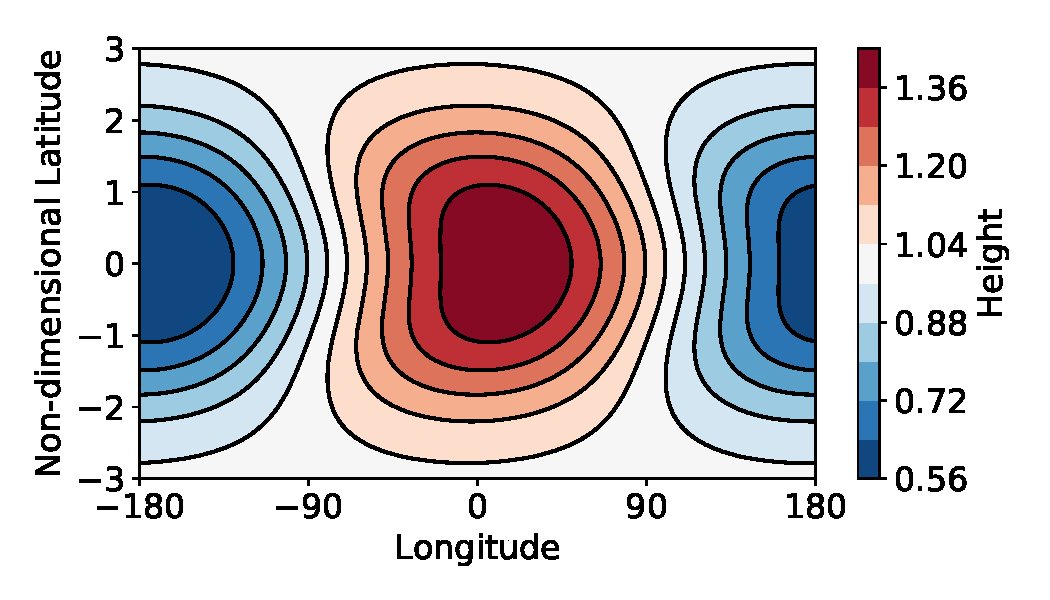
\includegraphics[width=1.0\textwidth]{figures/wave-mean-flow/beta-damping.pdf}
    \caption{Zero background flow and damping $\alpha = 1.0$.}
    \label{fig:alpha-dominates-shift}
  \end{subfigure}
  \quad
  \begin{subfigure}[t]{0.30\textwidth}
    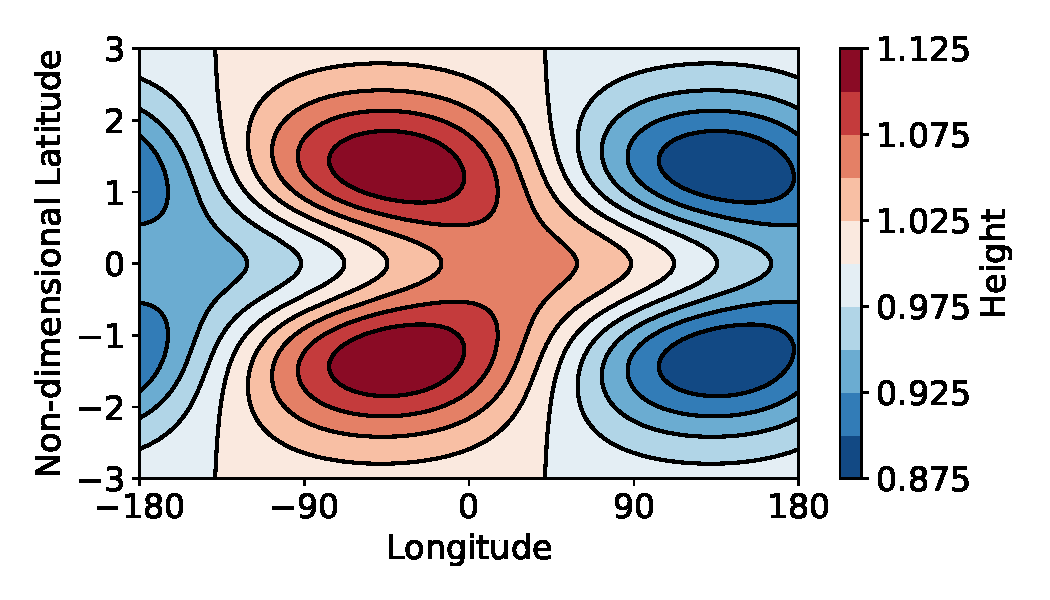
\includegraphics[width=1.0\textwidth]{figures/wave-mean-flow/beta-eigenvalue.pdf}
    \caption{Zero background flow and damping $\alpha = 0.2$.}
    \label{fig:eigenvalue-dominates-shift}
  \end{subfigure}
  \quad
  \begin{subfigure}[t]{0.30\textwidth}
    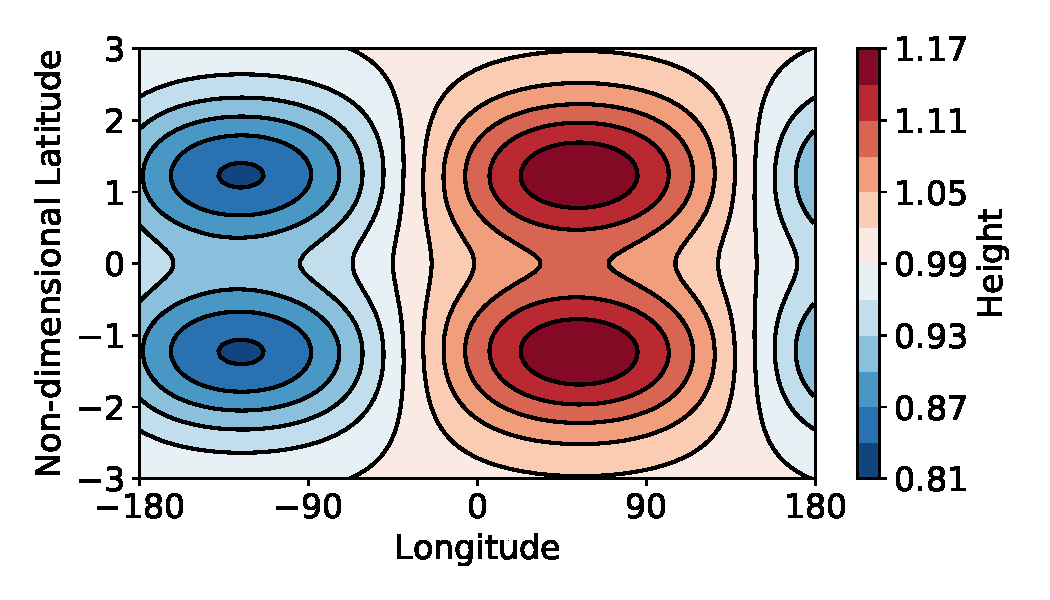
\includegraphics[width=1.0\textwidth]{figures/wave-mean-flow/beta-flow.pdf}
    \caption{Background flow $U_{0}=0.5$ and damping $\alpha = 0.2$.}
    \label{fig:flow-dominates-shift}
  \end{subfigure}
  \caption{The linear responses to a forcing  with magnitude $Q_{0}=1.0$ and $\alpha=0.2$ unless specified. The positions of the various modes depends on the terms in the denominator of Equation \ref{eqn:am-U0}.}
  \label{fig:U0-shift-demo}
\end{figure}



% %SUBSECTION -- SHEAR FLOW
% \subsection{Shear Background Flow}

%For the forced response to be similar to the results of GCM simulations like those in Figure \ref{fig:example-gcm-results}, the strength of the height perturbation $\overline{H}(y)=-y\overline{U}(y)$ from the jet $\overline{U}(y)$ must be comparable to the strength of the height perturbation $\alpha_{rad}Q(y)$ from the forcing $Q(y)$.


%SECTION CONCLUSIONS


%%%%%%%%%%%%%%%%%%%%%%%%%%%%%%%%%%%%
%SECTION 2 -- SHEAR FLOW ON BETA-PLANE
\section{Free Modes in Shear Flow on the Beta-Plane}\label{sec:shear-flow-beta-plane}

% In this section, I discuss the main result of this chapter -- the forced response of the shallow-water equations linearized around a zonally uniform shear flow $\overline{U}(y)$ and height $\overline{H}(y)$. I will show that the form of this forced response matches the results of GCM simulations, and suggest that the equatorial jet is therefore vital in controlling the global temperature structure and circulation pattern.

This section investigates the free modes of the shallow-water equations linearised about a shear background flow $\overline{U}(y)$ and the associated geostrophically balanced height perturbation $\overline{H}(y)$. I will show how the flow affects these free modes, which will be important later in understanding the response to forcing in a shear flow.

% The background flow $\overline{U}(y)$ and height $\overline{H}(y)$ satisfy the second line of Equation \ref{eqn:sw-eqns-R}, so are geostrophically balanced with $\overline{H}_{y}(y)=-y\overline{U}(y)$. For our Gaussian jet $\overline{U}(y)=U_{0}e^{-y^{2}/2}$, the height perturbation is therefore $\overline{H}(y)=U_{0}e^{-y^{2}/2}$ \citep{hammond2018wavemean}.

The shallow-water systems in this section have a forcing magnitude $Q_{0}=1$ and equal radiative and dynamical damping rates $\alpha_{rad}=\alpha_{dyn} = 0.2$ \citep{matsuno1966quasi}. Section \ref{sec:effect-damping-rate} will show the effect of varying these damping rates. The tests in this section show the effect of a zonal flow with a maximum non-dimensional speed between 0 and 1, which was shown previously to be the speed required for a significant zonal shift of the stationary waves. The value of $Q_{0}=1$ in the forcing $Q(y)=Q_{0}\sin(x)e^{-y^{2}/2}$ was chosen to be the same as \citet{matsuno1966quasi} and \citet{showman2011superrotation}, and also to produce stationary waves with similar magnitudes to the strength of the imposed zonal jet.

% In Section XX I will use a different forcing value, to satisfy this condition in a spherical geometry with a different balance between jet velocity and jet height.
%
% In this section, I will discuss the effect of a background shear flow on the free modes of the shallow-water equations. This will be useful to understand the effect of the background flow on the forced response, in the next section.

Section \ref{sec:shallow-water} showed how an exact solution for the response to a forcing can be written as a sum of the free modes of the system. An exact solution is not possible when the system is linearised about a background flow $\overline{U}(y)$ and $\overline{H}(y)$, but it is still useful to interpret the approximate solution in terms of the fundamental free modes. I will write the free solutions to the shallow-water equations as complex functions of latitude $A(y)$, and the forced solutions as functions of both latitude and longitude in the form $A(y) e^{i \delta(y) x}$. The function $\delta(y)$ determines the longitudinal structure of the forced response, and is equivalent to the phase shift $(\omega_{m} - k_{x} \overline{U})$ derived earlier for a uniform background flow.

The response to forcing can still be interpreted as a sum of the free modes of the system. The free modes of this system linearised about a shear flow have a different latitudinal structure $u(y),v(y),h(y)$ and different eigenvalues $\omega_{m}$, so will have different longitudinal positions in the forced response. Linearised around the background flow $\overline{U}(y)$ and height $\overline{H}(y)$, the shallow-water equations are:

\begin{equation}\label{eqn:shear-sw-equations}
    \begin{gathered}
      \frac{\partial u}{\partial t} +  \alpha_{dyn} u + \frac{\partial \overline{U}(y)u}{\partial x} +(\frac{\partial \overline{U}(y)}{\partial y} - y)v + \frac{\partial h}{\partial x} = 0, \\
      \frac{\partial v}{\partial t} +  \alpha_{dyn} v + \frac{\partial \overline{U}(y)v}{\partial x} + y u + \frac{\partial h}{\partial y} = 0, \\
      \frac{\partial \overline{H}' u}{\partial x} + \overline{H}'\frac{\partial v}{\partial y} - y\overline{U}(y) v +\frac{\partial h}{\partial t} +  \alpha_{rad} h + \frac{\partial \overline{U}(y) h}{\partial x} = Q(y), \\
        \overline{H}' = 1+\overline{H}(y).
    \end{gathered}
\end{equation}


The free modes of Equation \ref{eqn:shear-sw-equations} are found by setting $Q(y)=0$ and $\partial /\partial t = -i \omega$, and writing $u,v,h$ in the form $A(y) e^{i(k_{x}x - \omega t)}$. Casting the resulting equations in a matrix form gives:


  \begin{equation}\label{eqn:free-sw-shear}
    \begin{gathered}
      \begin{pmatrix}
      \alpha_{dyn} + i k_{x}\overline{U}(y) & \frac{\partial\overline{U}(y)}{\partial y}-y & i k_{x} \\
      y & \alpha_{dyn} + i k_{x}\overline{U}(y) & \frac{\partial}{\partial y} \\
      i k_{x} \overline{H}' & -y \overline{U}(y) + \overline{H}' \frac{\partial}{\partial y} & \alpha_{rad} + k_{x}\overline{U}(y)
      \end{pmatrix}
      \begin{pmatrix}
      u \\
      v \\
      h
      \end{pmatrix}
      =
      i \omega
      \begin{pmatrix}
      u \\
      v \\
      h
      \end{pmatrix}, \\
        \overline{H}' = 1+\overline{H}(y).
    \end{gathered}
  \end{equation}

% I solved both the free and forced systems of equations using the method in Appendix X, expanding the solutions in terms of the parabolic cylinder functions. This method identifies the exact free and forced solutions in the case where $\overline{U}(y)=0$, and finds the solutions with non-zero $\overline{U}(y)$ to better than 1 part in 10,000 when 30 basis modes are used in the calculation. In Appendix X, I show the accuracy of this method in more detail.

The background state of $\overline{U}(y)$ and $\overline{H}(y)$ must satisfy Equation \ref{eqn:shear-sw-equations} by itself. On the beta-plane, this means that the shear flow $\overline{U}(y)$ is geostrophically balanced by the height perturbation $\overline{H}(y)$. The second line of Equation \ref{eqn:shear-sw-equations} requires that for a background flow $\overline{U}(y)$, the background state is:

\begin{equation}\label{eqn:sw-eqns-1}
  \begin{gathered}
\overline{U}(y) =  U_{0} e^{-y^{2}/2} \\
\overline{V}(y) =  0 \\
\overline{H}(y) =  U_{0} e^{-y^{2}/2} \\
  \end{gathered}
\end{equation}

In this model, the perturbations in the forced system apply to a single shallow-water layer of height $H_{0}$ (which is non-dimensionalised to unity). The vertically varying heating profile in a planetary atmosphere technically excites a continuum of vertical modes, each defining a shallow-water system of different $H_{0}$. However, \citet{tsai2014three} showed that almost all the energy is confined to the lowest-order vertical mode in this forced shallow-water system, so this approximation by a single layer is reasonable.

 % Appendix \ref{sec:app-beta} shows the accuracy of this method, demonstrating that the pseudo-spectral method identifies the exact solution in the case with no background jet, and that the solution with a background flow changes by less than 1 part in 10,000 for any modes past $n=30$. The pseudo-spectral method finds $N_{m}$ solutions (the number of modes used in the calculation) for the eigenvalue equation governing the free modes. Many of these are spurious, but we can distinguish them from the physical modes by inspecting their eigenvalues. The pseudo-spectral method only produces a single solution for the forced linear system, which is simpler to interpret.



\begin{figure}
  \centering
  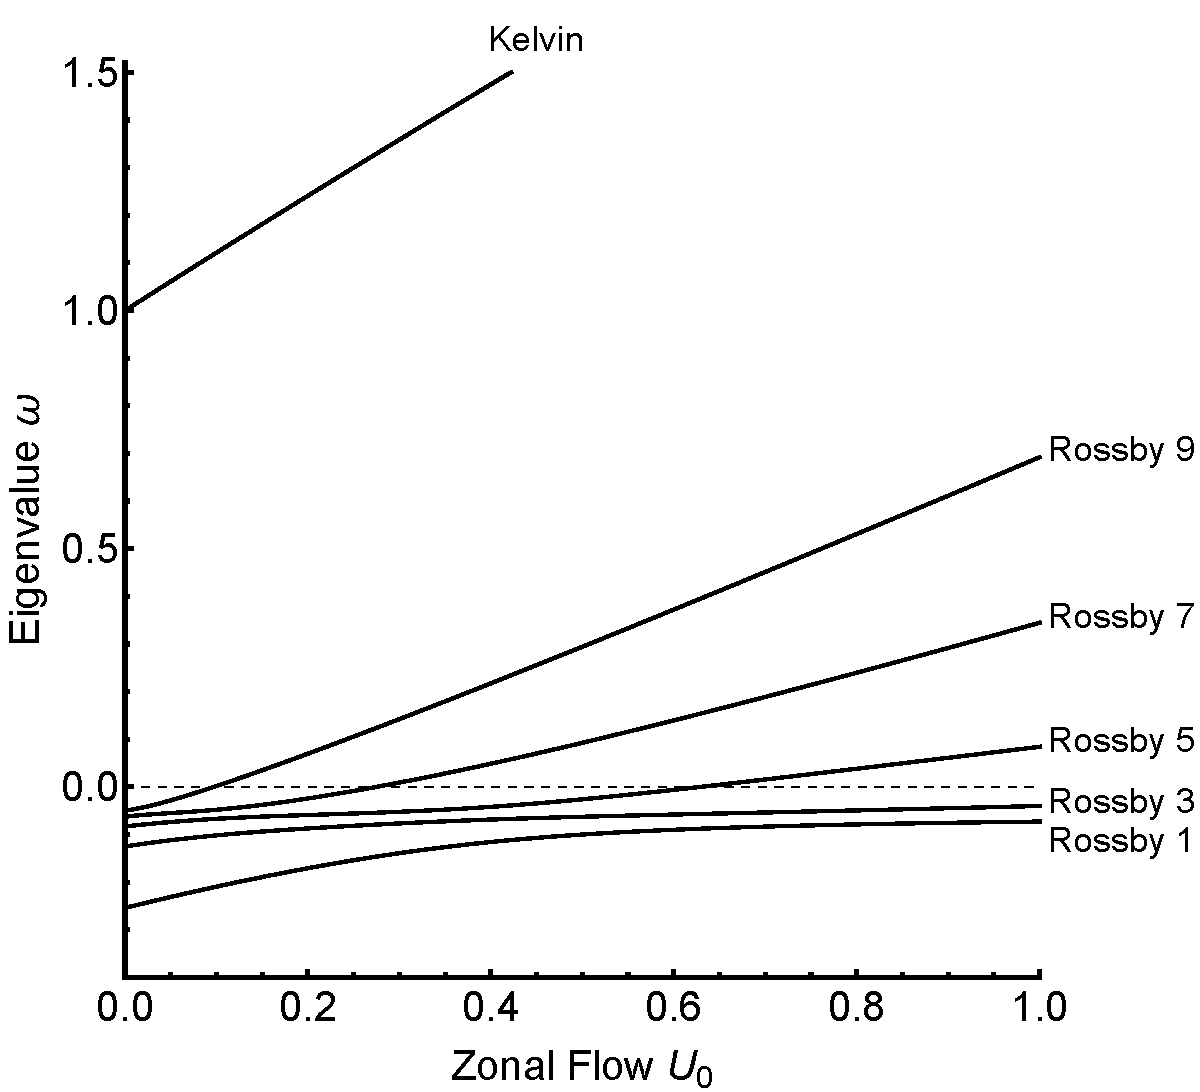
\includegraphics[width=0.55\textwidth]{figures/wave-mean-flow/shear-flow-eval-shift.pdf}
  \caption{The eigenvalues of the free modes of Equation \ref{eqn:free-sw-shear}, showing how eastward flow makes the eigenvalues more positive, corresponding to an eastward shift in the response to forcing.}
  \label{fig:shear-flow-eval-shift}

\vspace*{1.2cm}

  \begin{subfigure}[b]{0.32\textwidth}
    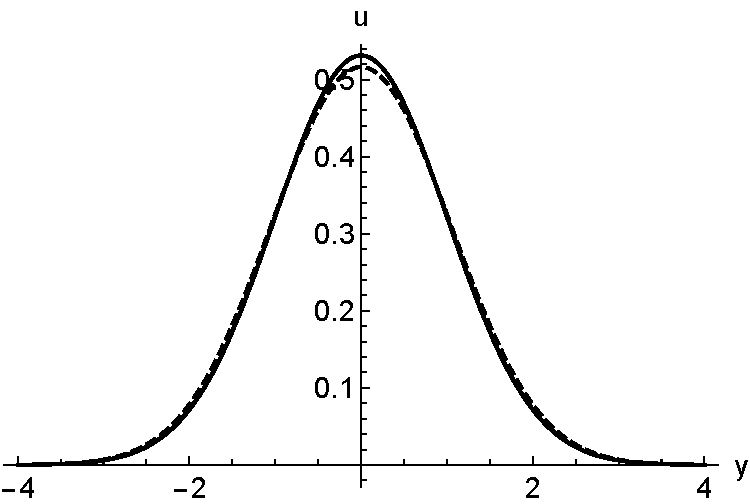
\includegraphics[width=\textwidth]{figures/wave-mean-flow/free-u-shear-kelvin.pdf}
    \caption{Zonal velocity.}
    \label{fig:free-u-shear-kelvin}
  \end{subfigure}
  %
  \begin{subfigure}[b]{0.32\textwidth}
    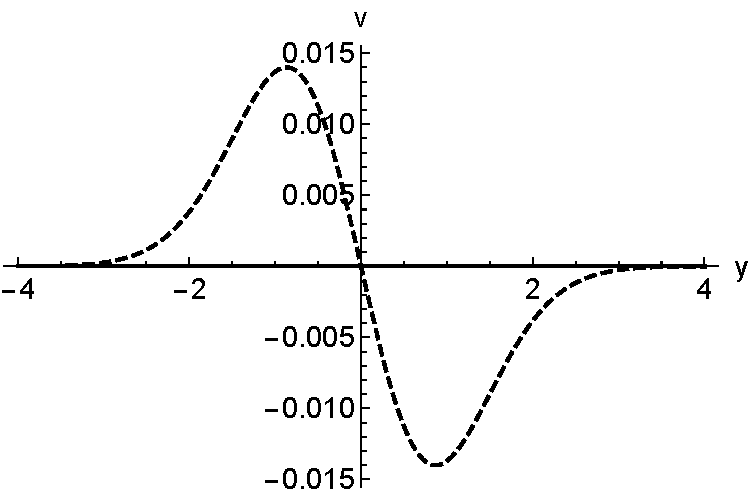
\includegraphics[width=\textwidth]{figures/wave-mean-flow/free-v-shear-kelvin.pdf}
    \caption{Meridional velocity.}
    \label{fig:free-v-shear-kelvin}
  \end{subfigure}
  %
  \begin{subfigure}[b]{0.32\textwidth}
    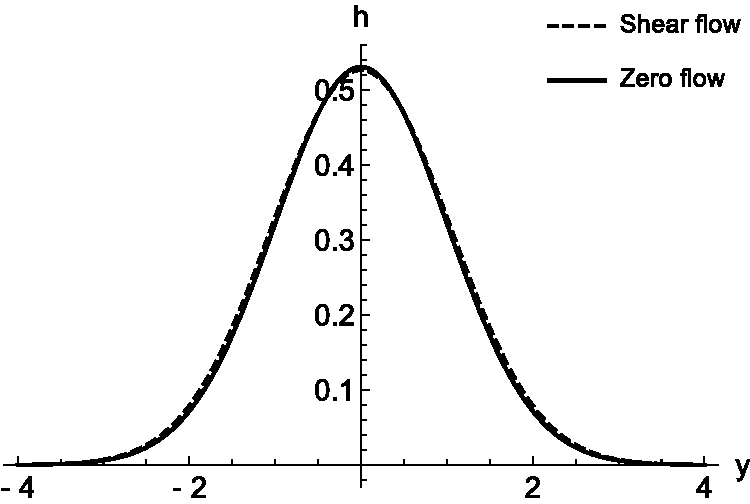
\includegraphics[width=\textwidth]{figures/wave-mean-flow/free-h-shear-kelvin.pdf}
    \caption{Height.}
    \label{fig:free-h-shear-kelvin}
  \end{subfigure}
  %
  \caption{The meridional structure of the free Kelvin mode, with and without a background shear flow \citep{hammond2018wavemean}. The flow introduces a non-zero meridional velocity.}
  \label{fig:free-shear-meridional-kelvin}

\vspace*{1.2cm}

%


  \begin{subfigure}[b]{0.32\textwidth}
    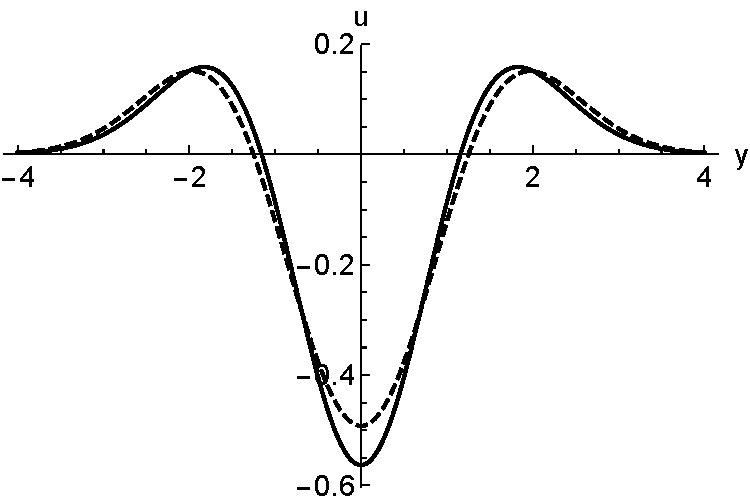
\includegraphics[width=\textwidth]{figures/wave-mean-flow/free-u-shear.pdf}
    \caption{Zonal velocity.}
    \label{fig:free-u-shear}
  \end{subfigure}
  %
  \begin{subfigure}[b]{0.32\textwidth}
    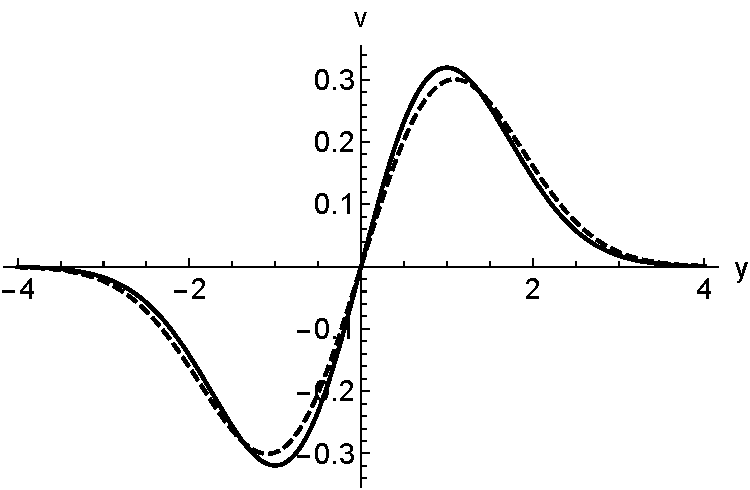
\includegraphics[width=\textwidth]{figures/wave-mean-flow/free-v-shear.pdf}
    \caption{Meridional velocity.}
    \label{fig:free-v-shear}
  \end{subfigure}
  %
  \begin{subfigure}[b]{0.32\textwidth}
    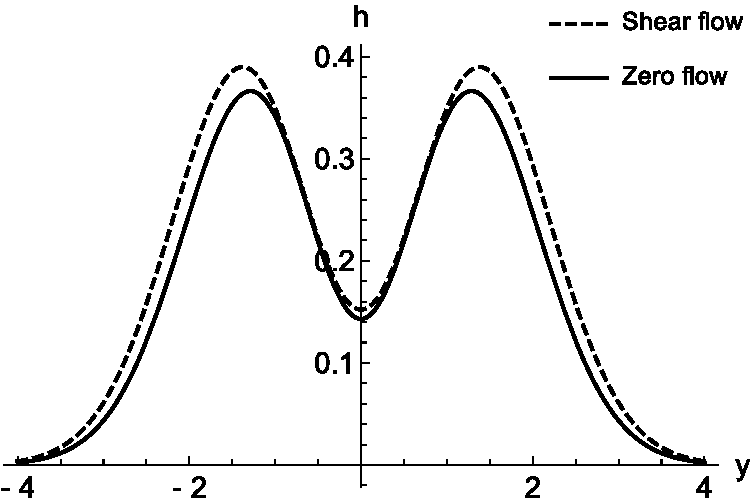
\includegraphics[width=\textwidth]{figures/wave-mean-flow/free-h-shear.pdf}
    \caption{Height.}
    \label{fig:free-h-shear}
  \end{subfigure}
  %
  \caption{The meridional structure of the free Rossby mode, with and without a background shear flow \citep{hammond2018wavemean}. The shear affects the meridional structure, effectively changing the $y$ coordinate \citep{boyd1978sheari}.}
  \label{fig:free-shear-meridional}
\end{figure}

% The shear affects the meridional structure, effectively changing the $y$ coordinate \citep{hammond2018wavemean}


% \newpage
%%%%%%%%



\subsection{Free Mode Eigenvalues}

Appendix \ref{ap:ps-methods} describes the methods used to find the free modes of the shallow-water system defined by Equation \ref{eqn:free-sw-shear} for a background flow $\overline{U}(y)=U_{0}e^{-y^{2}/2}$ \citep{hammond2018wavemean}. Figure \ref{fig:shear-flow-eval-shift} shows the real parts of the eigenvalues of the lowest-order (i.e. largest magnitude) modes excited by the symmetric, stationary forcing. These are the free Kelvin mode and the symmetric free Rossby modes of Equation \ref{eqn:free-sw-shear} \citep{matsuno1966quasi}. The value and sign of these eigenvalues determine the position of the free mode in the forced response, as discussed in Section \ref{sec:shallow-water}.

%Note that an exact forced solution in terms of a series of free modes is now not possible as the flow is not uniform, but it is still very useful to interpret the forced response in this way.

As the magnitude $U_{0}$ of the equatorial jet $\overline{U}(y)$ increases in Figure \ref{fig:shear-flow-eval-shift}, all the eigenvalues of the free modes become more positive. This corresponds to an eastward shift in their position in the forced response up to a maximum of \ang{+90} east, as in Equation \ref{eqn:am-U0}. The Kelvin mode has a positive eigenvalue for $U_{0}=0$, so is already east of the substellar point. This eigenvalue becomes larger as $U_{0}$ increases, so the Kelvin mode moves further east in the forced response.

The Rossby modes of different order $m$ shift by different amounts. \citet{tsai2014three} showed that in a uniform background flow, the $n=1$ Rossby mode is shifted eastwards towards \ang{+90}, producing the hot-spot shift (reproduced in Figure \ref{fig:U0-shift-demo}). In fact, Figure \ref{fig:shear-flow-eval-shift} shows that in this non-uniform flow $\overline{U}(y)$, the $n=1$ Rossby mode eigenvalue becomes less negative but does not become positive for $U_{0}=1.0$. This means that it is shifted east from its original position in the forced response, but is not shifted past the substellar point.

The higher order Rossby modes are shifted further past the substellar point by the flow $\overline{U}(y)$, as shown by their positive eigenvalues for high enough flow speed $U_{0}$. The modes of higher order are shifted further, but contribute less strongly to the forced response \citep{matsuno1966quasi}. Therefore, the response to forcing calculated below will be interpreted in terms of the free modes up to the $n=5$ symmetric Rossby mode, as the contribution of the higher-order modes is negligible.

The background shear flow also changes the latitudinal structure of each free mode. Figures \ref{fig:free-shear-meridional-kelvin} and \ref{fig:free-shear-meridional} show the lowest-order free solutions of Equation \ref{eqn:free-sw-shear}. These Kelvin and Rossby modes are slightly different to the free modes in zero background flow \citep{matsuno1966quasi}. The shear flow changes these solutions by adding higher order meridional structure, as discussed in more detail in \citet{boyd1978sheari}. In summary, the free modes respond to a shear zonal flow in a qualitatively similar way to the uniform zonal flow in Section \ref{sec:shallow-water}, but the details of their structure and shifts vary depending on the mode $m$.



%%%%%%%%

%
% That is not to say that the $n=1$ mode is never responsible for the hot-spot shift -- later, we will show that in a spherical geometry the $n=1$ mode shifts close to \ang{90} eastwards. It is also possible in the beta-plane system for different input parameters (flow speed, damping rates) to shift the $n=1$ Rossby mode past the substellar point. But, our free mode expansion has shown that the $n=1$ Rossby mode is not the only important mode, and that the higher-order modes are also important to the forced response.

\subsection{Unstable Modes}

 The eigenvalues of the free modes of this system come in pairs, if there is no damping. They have equal and opposite positive and negative imaginary parts. The modes with positive imaginary parts will grow unstably \citep{wang2014instability, ribstein2014instability}. For non-zero damping, the imaginary parts will become more negative, making some free modes stable for large enough damping.

Technically, these unstable modes mean that any linear initial value problem in this system is not well posed, as it will eventually be dominated by the most unstable modes rather than the stationary response discussed elsewhere. However, the non-linear shallow-water calculations and GCM simulations in other chapters show that the linear stationary response still appears to dominate. This suggests that in reality the unstable modes are strongly damped or reach equilibrium due to nonlinear effects. The free modes could cause time-variable behaviour in the atmospheres of tidally locked planets \citep{armstrong2017variability,pierrehumbert2018review}.


%%%%%%%%%%%%%%%%%%%%%%%%%%%%%%%%%%%%
%SECTION 3 -- FORCED SHEAR FLOW ON BETA-PLANE
\section{Forced Response in Shear Flow on the Beta-Plane}\label{sec:shear-flow-beta-plane}


\begin{figure}[t]
  \centering
    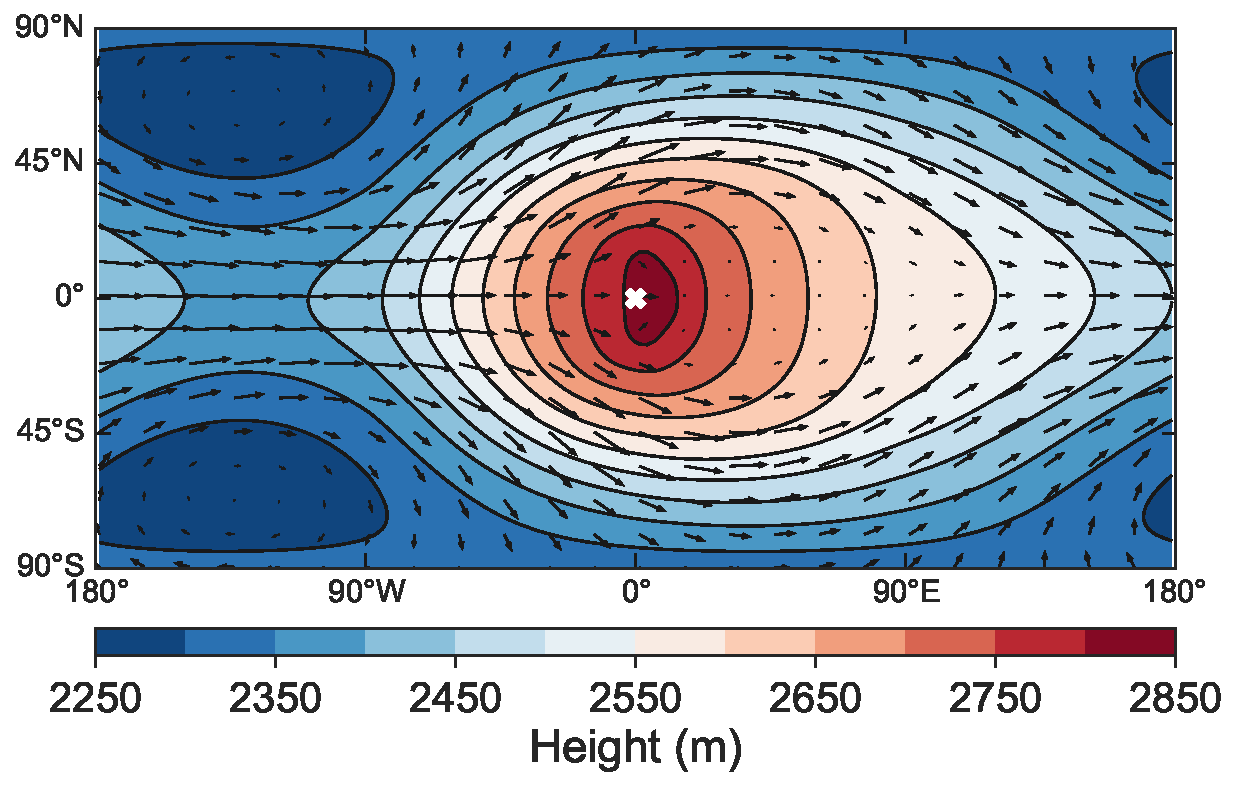
\includegraphics[width=0.7\textwidth]{figures/wave-mean-flow/example-gcm-results.pdf}
    \caption{The time-mean height field from a simulation of a tidally locked planet in the GCM Exo-FMS, showing the typical eastward equatorial jet, shifted hot-spot, and night-side stationary Rossby waves.}
    \label{fig:example-gcm-results}
\end{figure}

This section shows the effect of a background shear flow on the response to forcing in this linear model, which is the main result of this chapter. I will show the forced solutions with and without a background shear flow, discuss the form of the global circulation, and compare the shallow-water solutions to GCM simulations.

Figure \ref{fig:example-gcm-results} shows a GCM simulation of a tidally locked planet, with the features typical to such atmospheres. This planet is an idealised example of a terrestrial planet orbiting an M-dwarf, with radius $1.0\ R_{E}$ and orbital period of 10 Earth days. It has an $N_{2}$ atmosphere with surface pressure \SI{1}{\bar}. In the semi-grey radiative transfer scheme, it has a longwave optical thickness of $1$ and a shortwave optical thickness of $0$. The large-scale features of the global circulation are not sensitive to these parameters, and similar circulation patterns are seen in simulations of very different types of tidally locked planet \citep{showman2012review, heng2015review}.


%SUBSECTION --
\subsection{Response to Forcing}\label{sec:forcing-response}

The stationary response to steady forcing of Equation \ref{eqn:shear-sw-equations} is found by setting $Q(y)=Q_{0}e^{-y^{2}/2}$ \citep{matsuno1966quasi} and $\partial / \partial t = 0 $, giving the linear system of equations:


\begin{equation}\label{eqn:forced-sw-shear}
  \begin{gathered}
    \begin{pmatrix}
    \alpha_{dyn} + i k_{x}\overline{U}(y) & \frac{\partial\overline{U}(y)}{\partial y}-y & i k_{x} \\
    y & \alpha_{dyn} + i k_{x}\overline{U}(y) & \frac{\partial}{\partial y} \\
    i k_{x}\overline{H}' & -y \overline{U}(y) + \overline{H}' \frac{\partial}{\partial y} & \alpha_{rad} + k_{x}\overline{U}(y)
    \end{pmatrix}
    \begin{pmatrix}
    u \\
    v \\
    h
    \end{pmatrix}
    =
    \begin{pmatrix}
    0 \\
    0 \\
    Q(y)
    \end{pmatrix}, \\
      \overline{H}' = 1+\overline{H}(y).
  \end{gathered}
\end{equation}

 The eastward zonal flow is $\overline{U}(y) = U_{0} e^{-y^{2}/2}$, where $U_{0}$ is a free parameter. The equatorial Rossby radius of the planet sets the meridional scale of the beta-plane system, and by extension the scale of the forcing and width of the jet. This means that this beta-plane solution is limited to planets where the equatorial Rossby radius is comparable to the planetary radius and the width of the jet. These conditions are met on many realistic tidally locked planets, making the beta-plane solution a useful approximation \citep{pierrehumbert2018review}. I will extend the solution to a spherical geometry without these limitations later in this chapter.

For the stationary solutions in this section, the non-dimensional damping rate is $\alpha = 0.2$ \citep{matsuno1966quasi} and the non-dimensional forcing magnitude is $Q_{0} = 1.0$. The magnitude of the zonal flow $U_{0}$ is varied between $0$ and $1$, as it was shown earlier that $U_{0} \sim 1$ is required for a significant hot-spot shift. As in Section \ref{sec:shear-flow-beta-plane}, the geostrophically balanced background state is $\overline{U}(y) =  U_{0} e^{-y^{2}/2}$ and $\overline{H}(y) =  U_{0} e^{-y^{2}/2}$. Solving Equation \ref{eqn:forced-sw-shear} with the method described in Appendix \ref{ap:ps-methods} gives the $u$, $v$, and $h$ fields that satisfy these equations.

\begin{figure}
  \centering
  \begin{subfigure}[t]{0.48\textwidth}
    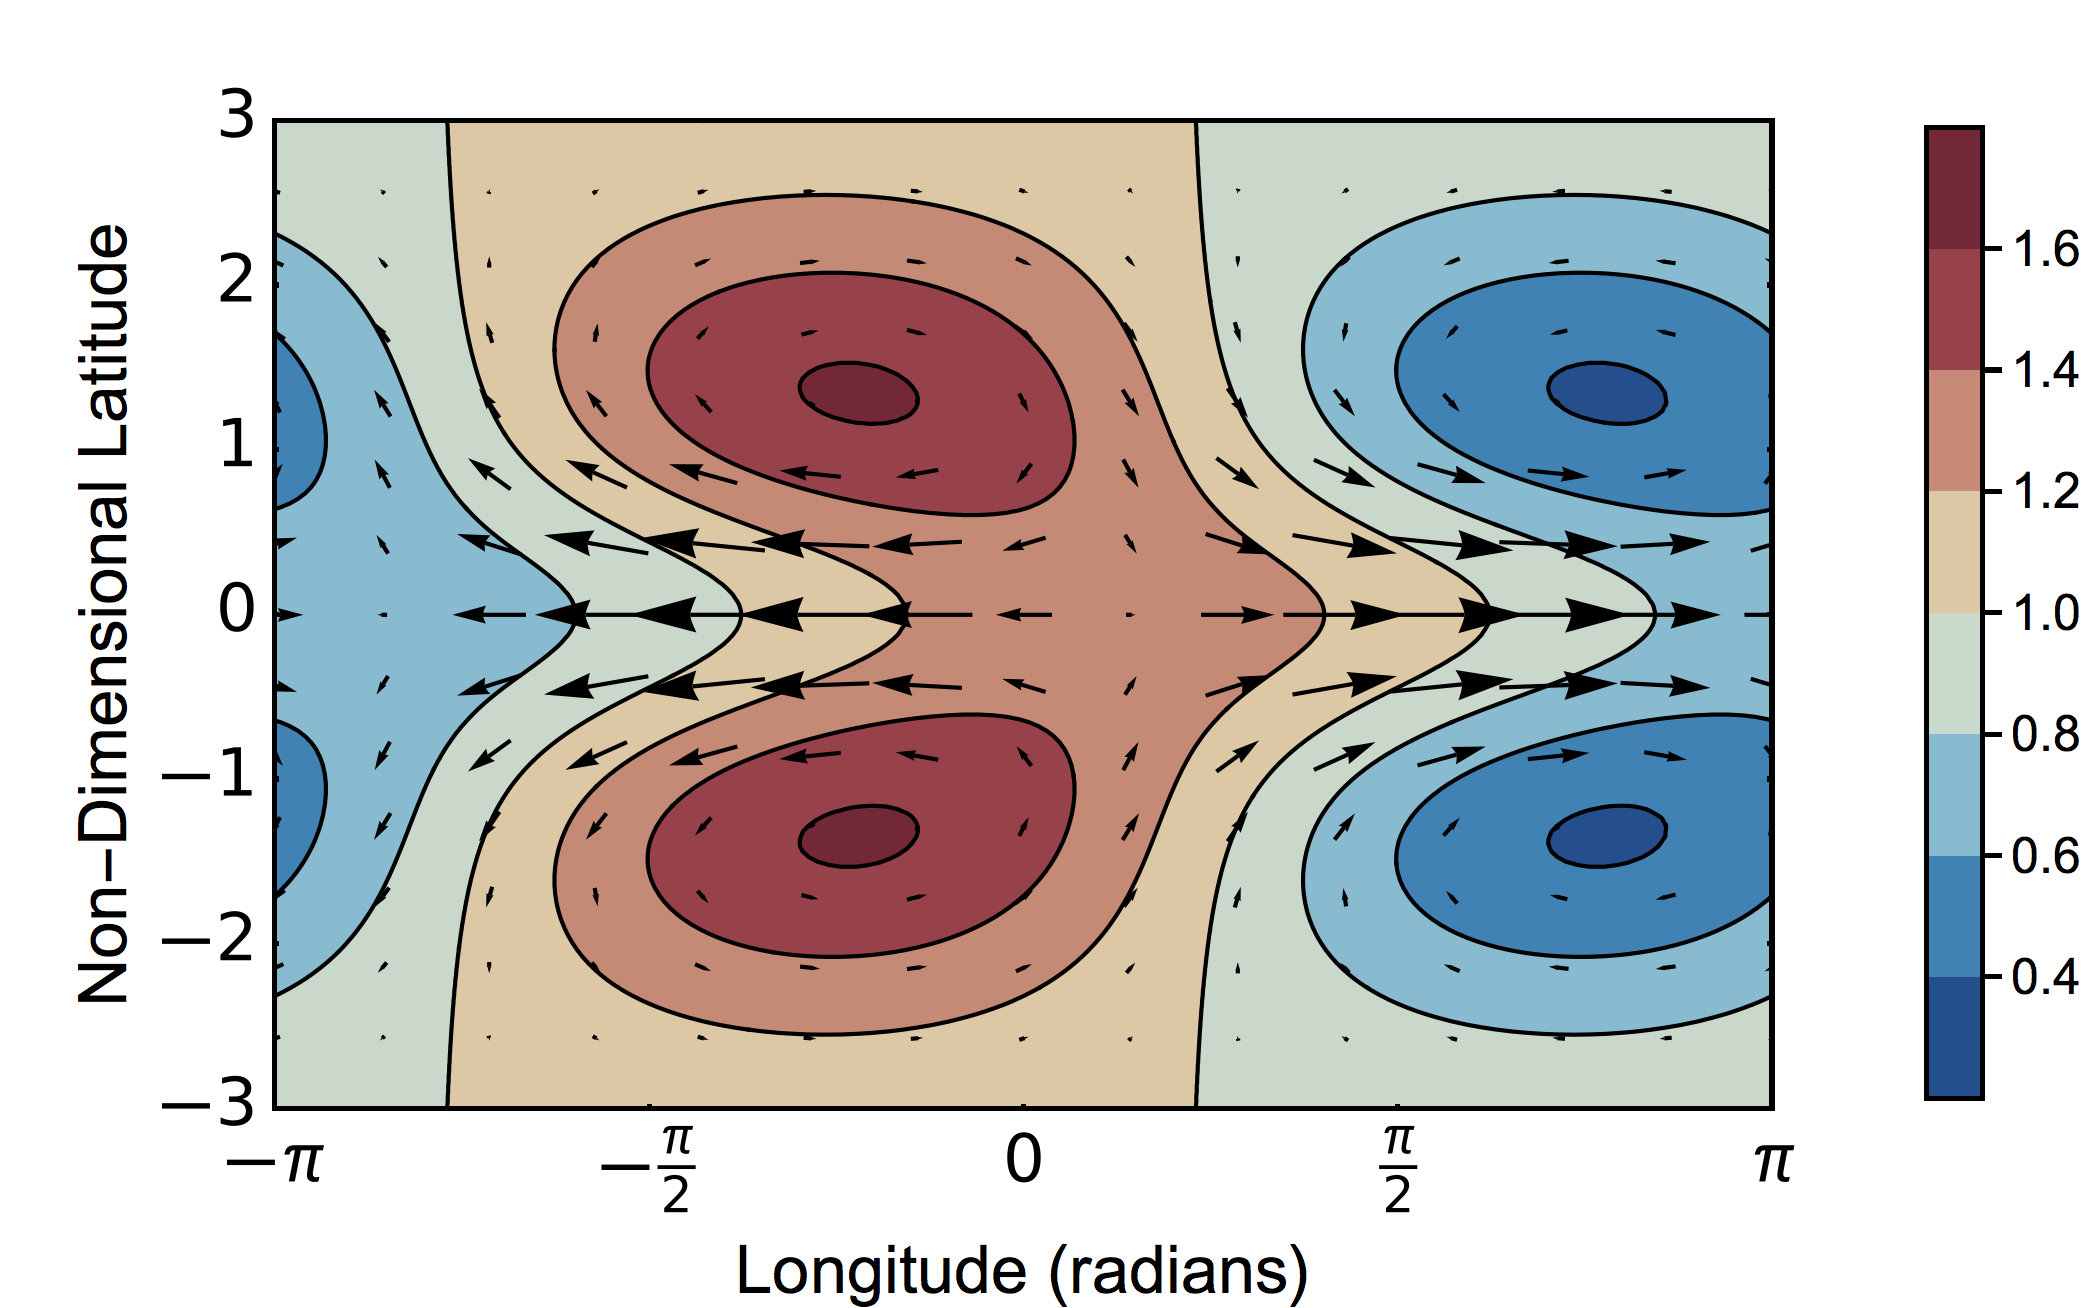
\includegraphics[width=\textwidth]{figures/wave-mean-flow/ps-no-flow.png}
    \caption{The response to forcing in zero background flow \citep{matsuno1966quasi}.}
    \label{fig:ps-no-flow}
  \end{subfigure}
\quad
  \begin{subfigure}[t]{0.48\textwidth}
    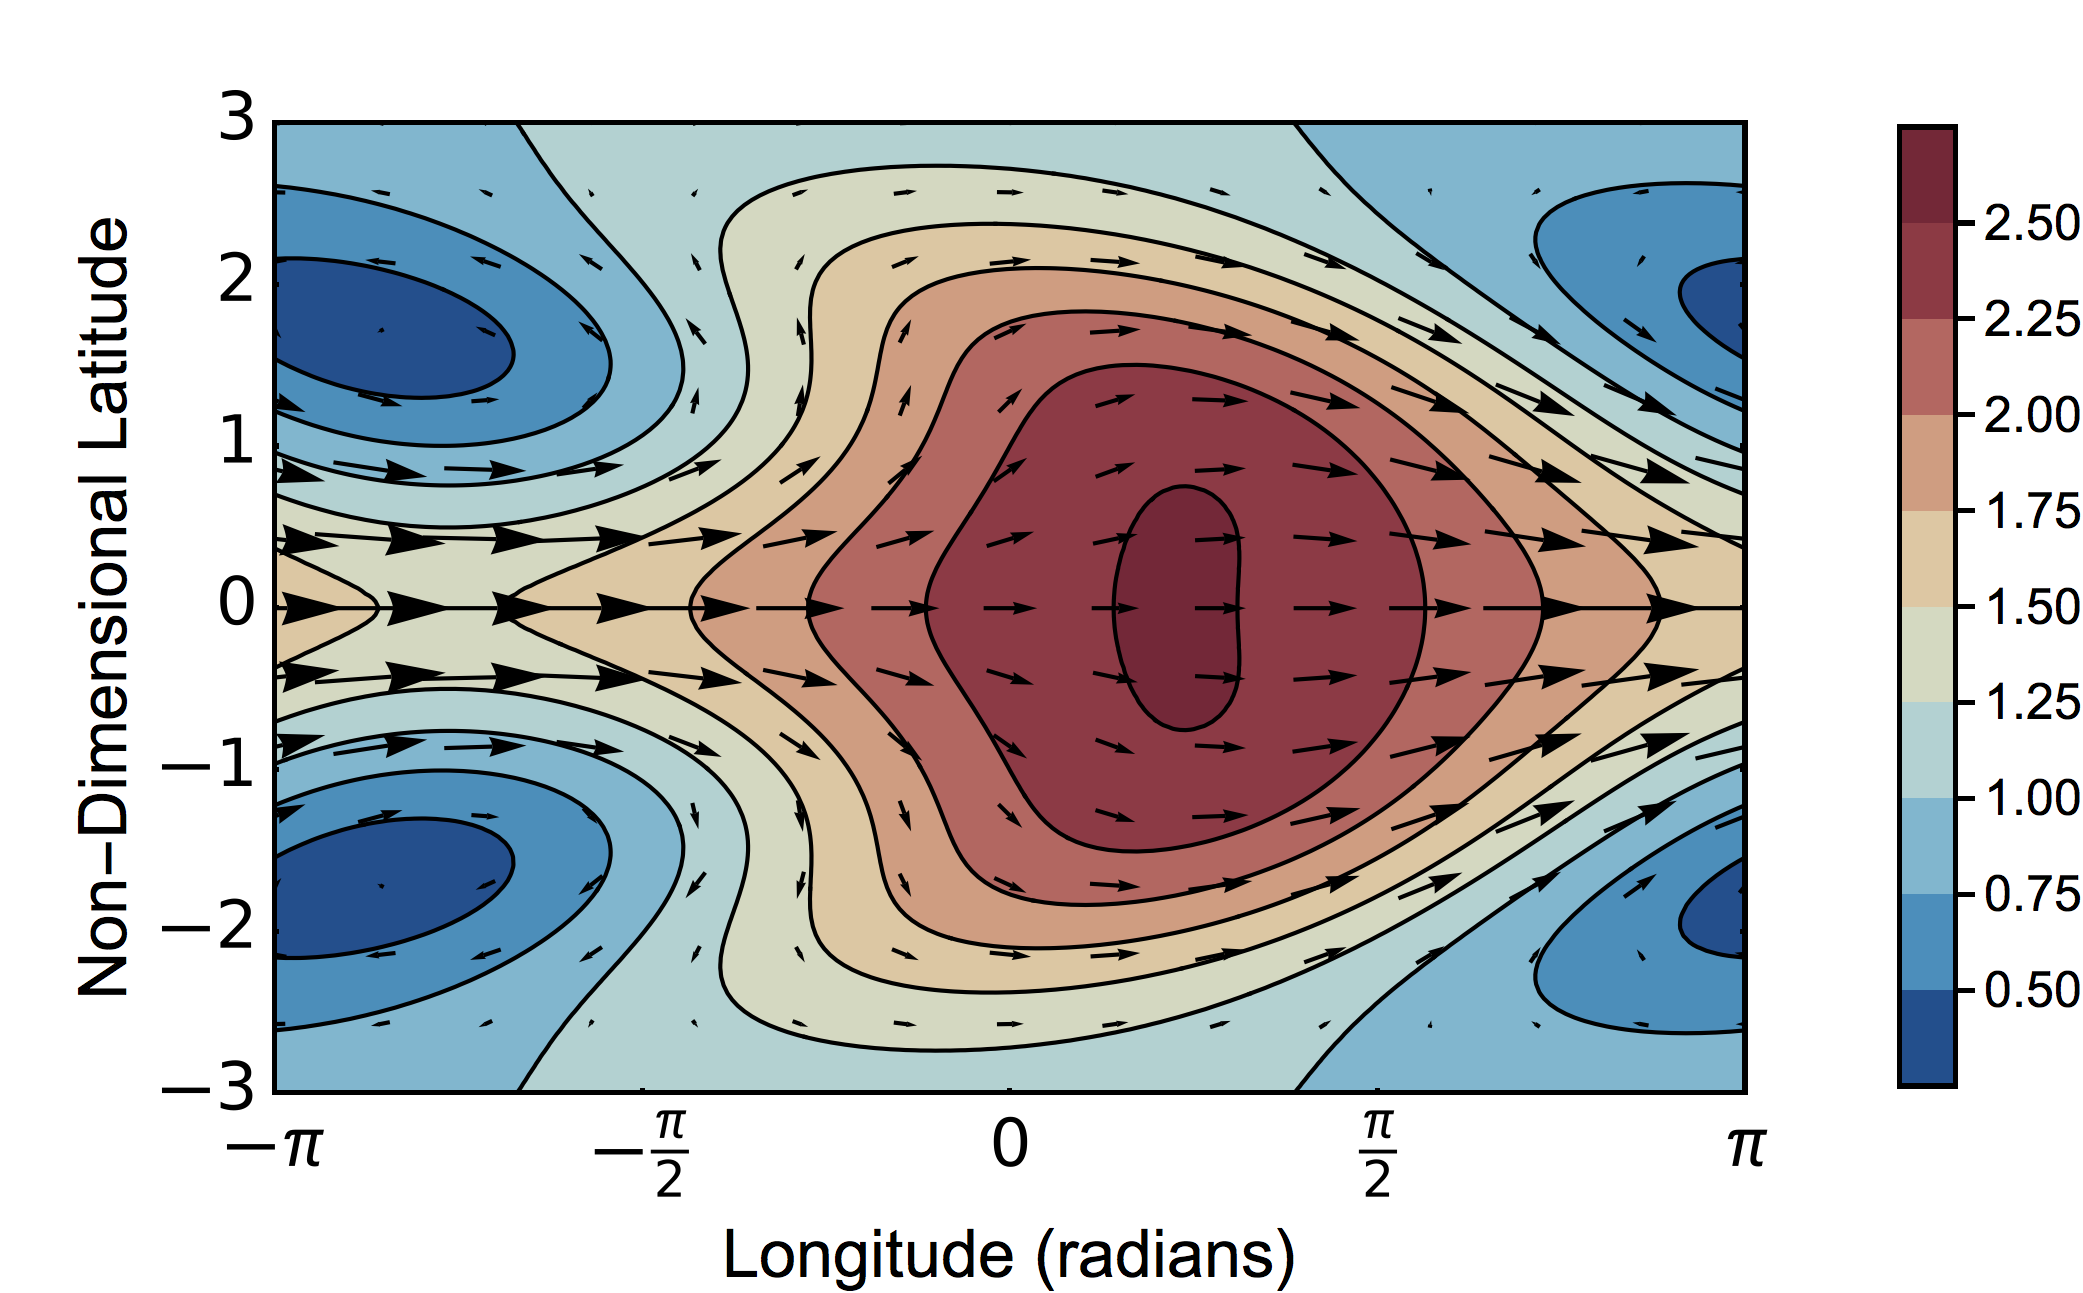
\includegraphics[width=\textwidth]{figures/wave-mean-flow/ps-shear-flow.png}
    \caption{The response to forcing in background flow $\overline{U}(y) =  U_{0} e^{-y^{2}/2}$, $U_{0}=1.0$.}
    \label{fig:ps-shear-flow}
  \end{subfigure}
  \caption{The effect of a background shear flow $\overline{U}(y)$ on the forced solutions of Equation \ref{eqn:forced-sw-shear}. The eastward flow Doppler-shifts the maximum of the response eastwards, producing the hot-spot shift seen in GCM simulations \citep{tsai2014three}.}
  \label{fig:ps-flow}
\end{figure}

Figure \ref{fig:ps-flow} shows the effect of the shear flow $\overline{U}(y)$ on the response to day-night forcing. This is the main result of this chapter, as it shows how the flow produces the global circulation pattern on a tidally locked planet in Figure \ref{fig:example-gcm-results}. The first plot, Figure \ref{fig:ps-no-flow}, shows the response to forcing in zero background flow. This is exactly the same as the linear solutions in \citet{matsuno1966quasi} and \citet{showman2011superrotation}, which were used in Chapter \ref{ch:eqm-zonal-flow} to calculate the initial acceleration of these atmospheres. This linear solution does not match the height field and velocities in Figure \ref{fig:example-gcm-results}. In particular, the ``hot-spot'' and cold (low height) Rossby waves are in different places in the shallow-water solution and in the GCM simulation.

The second plot, Figure \ref{fig:ps-shear-flow}, shows the response to forcing in the shear flow $\overline{U}(y)$ and height field $\overline{H}(y)$, which models the equilibrium state of the atmosphere. This qualitatively matches the GCM simulations in Figure \ref{fig:example-gcm-results}, with the ``hot-spot'' shifted east and the cold Rossby waves in the same places. I suggest that the solution in zero background flow in \citet{showman2011superrotation} predicts the initial acceleration of the atmosphere, which forms a zonal jet that modifies the response to day-night forcing, producing the global circulation pattern and the hot-spot shift as in \citet{tsai2014three}.

% This is consistent with \citet{tsai2014three}, who showed how a uniform background flow Doppler-shifts the forced waves eastwards, creating the hot-spot shift.

% See Chapter \ref{ch:eqm-zonal-flow} for a discussion of how the momentum fluxes in a tidally locked planetary atmosphere reach equilibrium, in the same way in shallow-water models and GCMs. The background flow $\overline{U}(y)$ imposed here approximates the zonal flow profile that gives equilibrium.




%SUBSECTION --
\subsection{Effect of Damping}\label{sec:effect-damping-rate}

The linear shallow-water model has several free parameters. I discussed the choice of the forcing strength $Q_{0}$ and jet speed $U_{0}$ earlier. The strengths of the free parameters $\alpha_{rad}$ and $\alpha_{dyn}$, the radiative and dynamical damping rates, affect the magnitude and form of the response to forcing. I previously showed that a very strong $\alpha_{rad}$ gives a response to forcing centred at the substellar point, but that for realistic radiative damping rates \citep{showman2011superrotation} the solution is similar to that in Figure \ref{fig:ps-flow}. The solution in Figure \ref{fig:ps-flow} assumed that $\alpha_{rad}$ and $\alpha_{dyn}$ were equal, which allows an analytic solution but is not physically justified.

The linear radiative damping $\alpha_{rad}$ has a realistic physical basis, but the linear dynamical damping $\alpha_{dyn}$ does not. It could be considered an approximation to effects like eddy viscosity, magnetohydrodynamic damping, or the effect of nonlinear terms \citep{heng2014analytical}. This section tests the effect of varying this damping rate, motivated by the uncertainty in the realism of a linear dynamical damping.

\begin{figure}
  \centering
  \begin{subfigure}[t]{0.48\textwidth}
    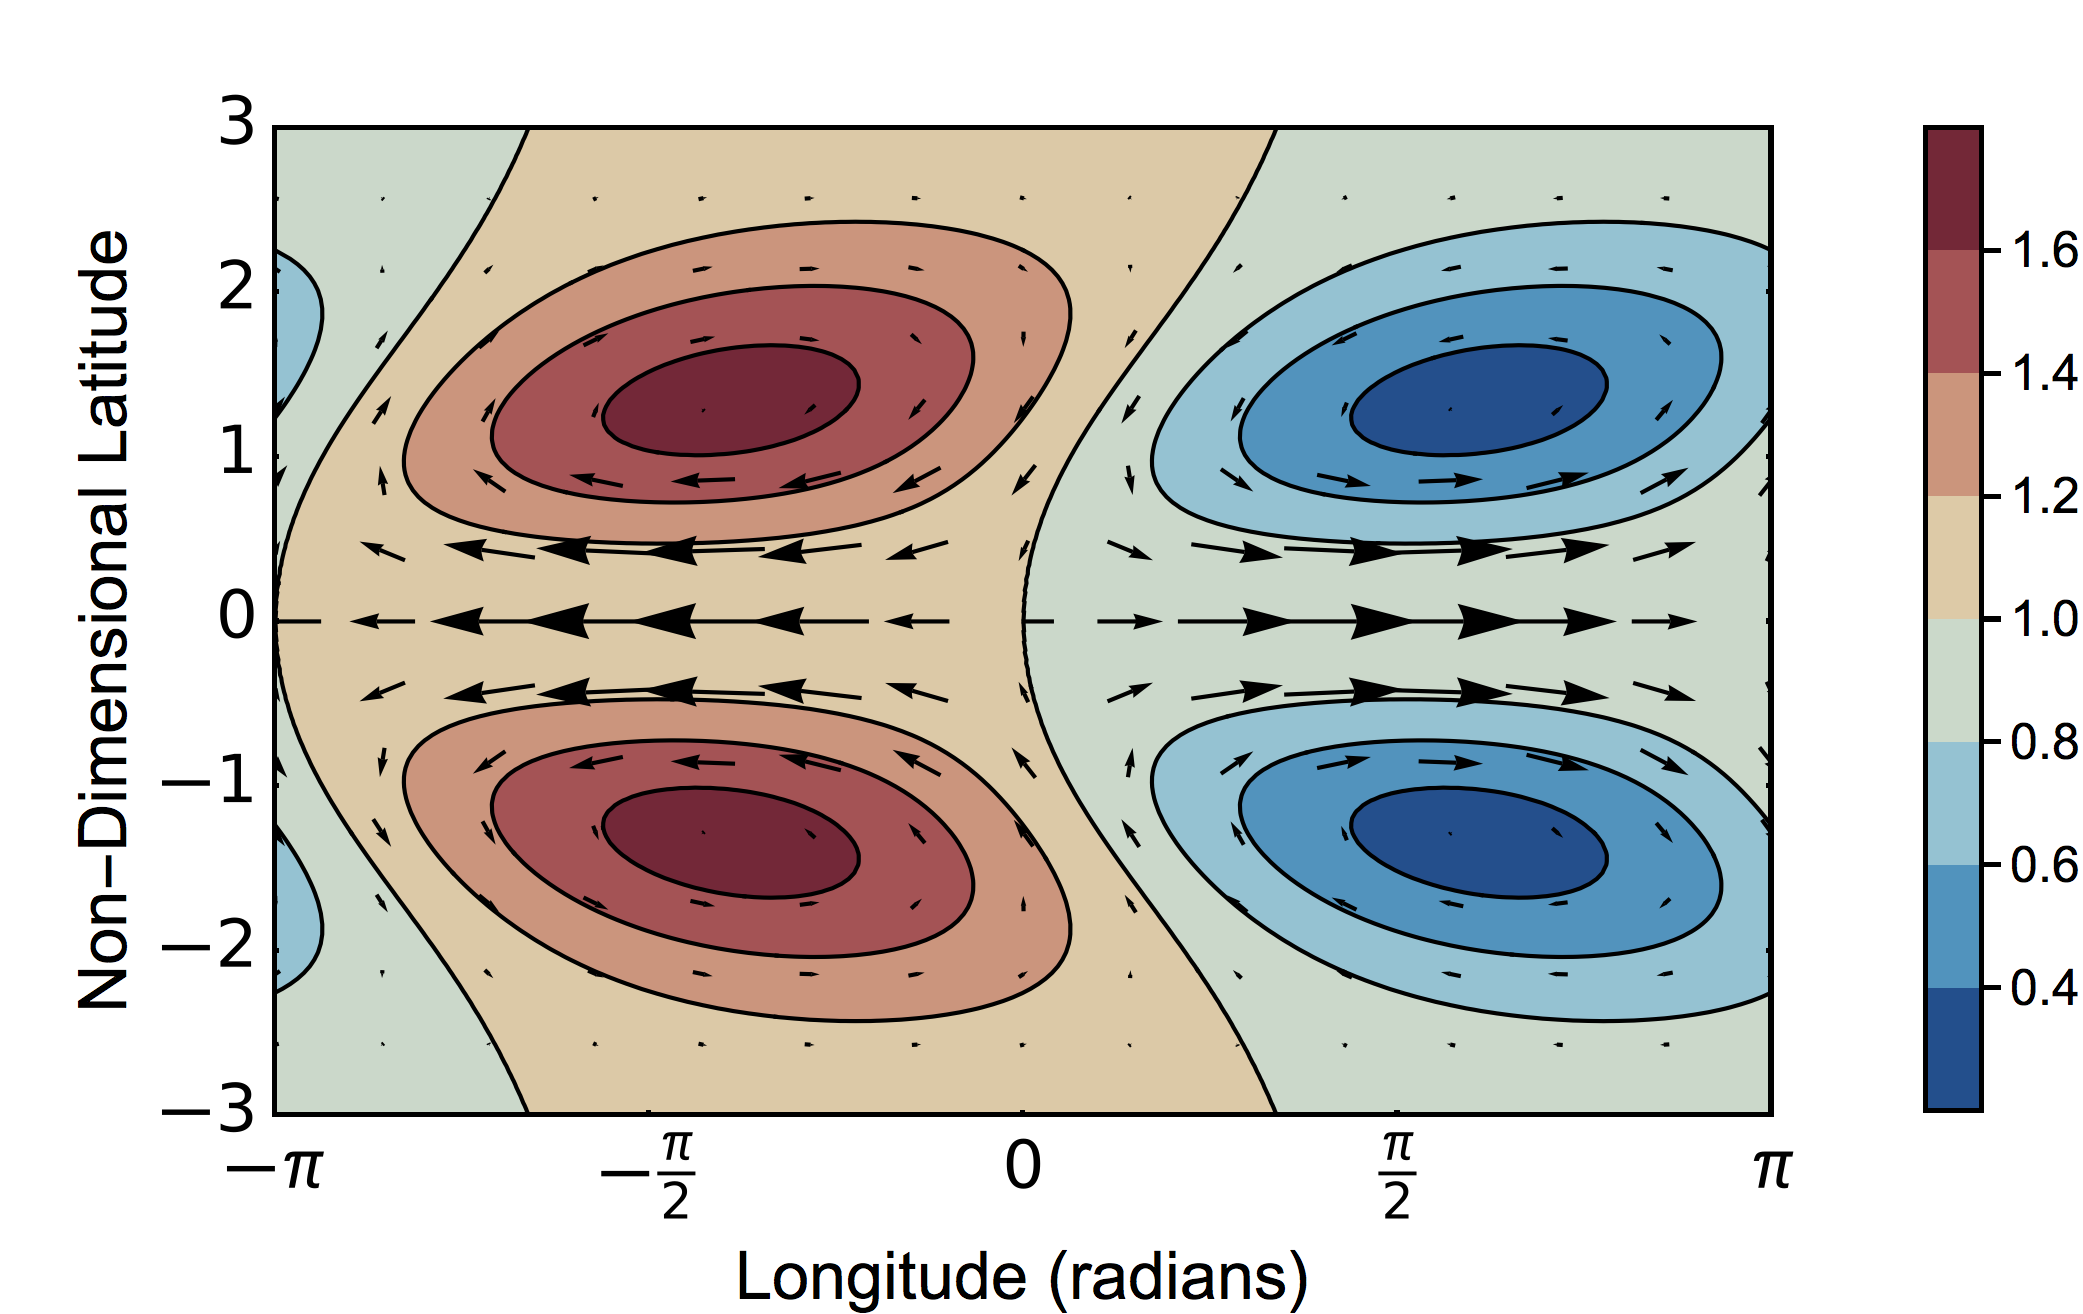
\includegraphics[width=\textwidth]{figures/wave-mean-flow/zero-alpha-dyn-zero-flow.png}
    \caption{Forced response in zero flow, with zero dynamical damping.}
    \label{fig:zero-alpha-dyn-zero-flow}
  \end{subfigure}
\quad
  \begin{subfigure}[t]{0.48\textwidth}
    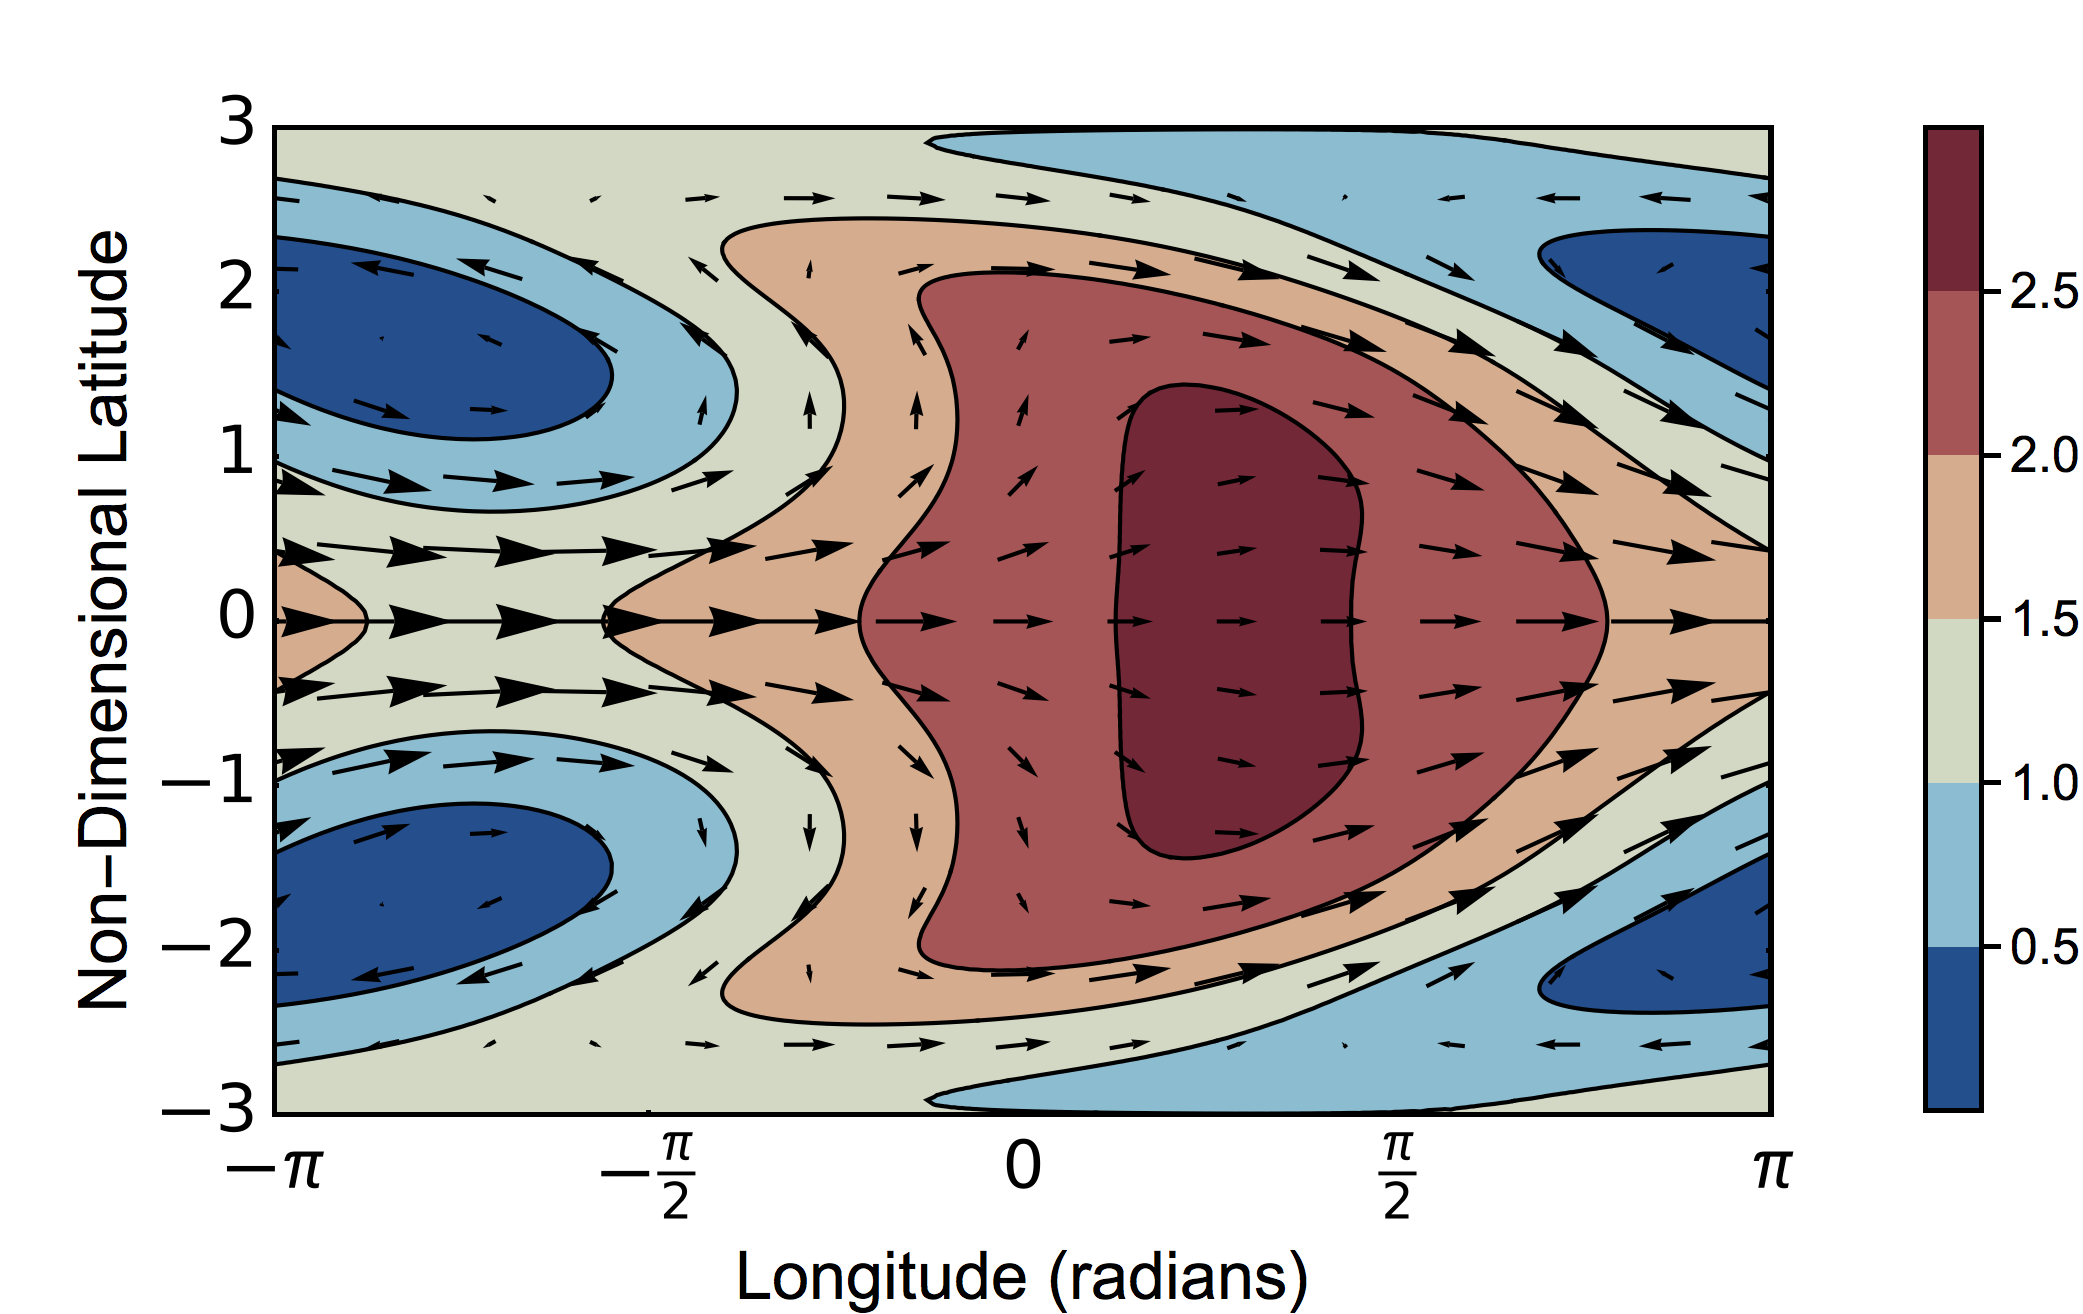
\includegraphics[width=\textwidth]{figures/wave-mean-flow/zero-alpha-dyn-1-flow.png}
    \caption{Forced response in shear flow $\overline{U}(y) =  U_{0} e^{-y^{2}/2}$, $U_{0}=1.0$.}
    \label{fig:zero-alpha-dyn-1-flow}
  \end{subfigure}
  \caption{The forced response in zero background flow and a shear background flow, for dynamical damping $\alpha_{dyn}=0$. These plots have the same form as those in Figure \ref{fig:ps-flow}, showing that the dynamical damping is not critical.}
  \label{fig:zero-alpha-dyn-flow}
\end{figure}

Figure \ref{fig:zero-alpha-dyn-flow} shows the response to forcing when the dynamical damping rate $\alpha_{dyn}$ is set to zero, with the same parameters as the solutions in Figure \ref{fig:ps-flow} otherwise. The first panel shows the solution in zero background flow, where the Kelvin response (the peak on the equator, in the previous plot) is now much weaker than the Rossby response (off the equator). The second panel shows the response to forcing in the shear background flow $\overline{U}(y) = U_{0} e^{-y^{2}/2}$ and associated height field $\overline{H}(y)$. This response is similar to the previous case with strong dynamical damping, showing that this damping is not a crucial part of the mechanism.

%This suggests that the uncertainty about the realism of this damping is not a problem for using the shallow-water model to explain the circulation of real planets.

% The solution has a similar form to that in Figure \ref{fig:ps-flow}, and importantly has a similar maximum on the equator, showing that the lack of equatorial response in the first panel is not an issue when a jet has formed.

% This presents problems for the acceleration mechanism discussed in Chapter \ref{ch:eqm-zonal-flow}, but in the GCM and in the non-linear shallow-water model in that chapter, there is always some Kelvin response -- so the dynamical damping represents some process at work in these.

The qualitative form of the forced solution does not depend strongly on the choice of the parameters $\alpha_{rad}$ and $\alpha_{dyn}$. The dynamical damping $\alpha_{dyn}$ does not have a clear physical basis, but is not strictly necessary to include to match the GCM simulations -- however, it is useful to include for a simpler solution that is closer to the analytic result in \citet{matsuno1966quasi}.



%SUBSECTION --
\subsection{Hot-Spot Shift Mechanism}


\begin{figure}
  \centering
  \begin{subfigure}[t]{0.48\textwidth}
    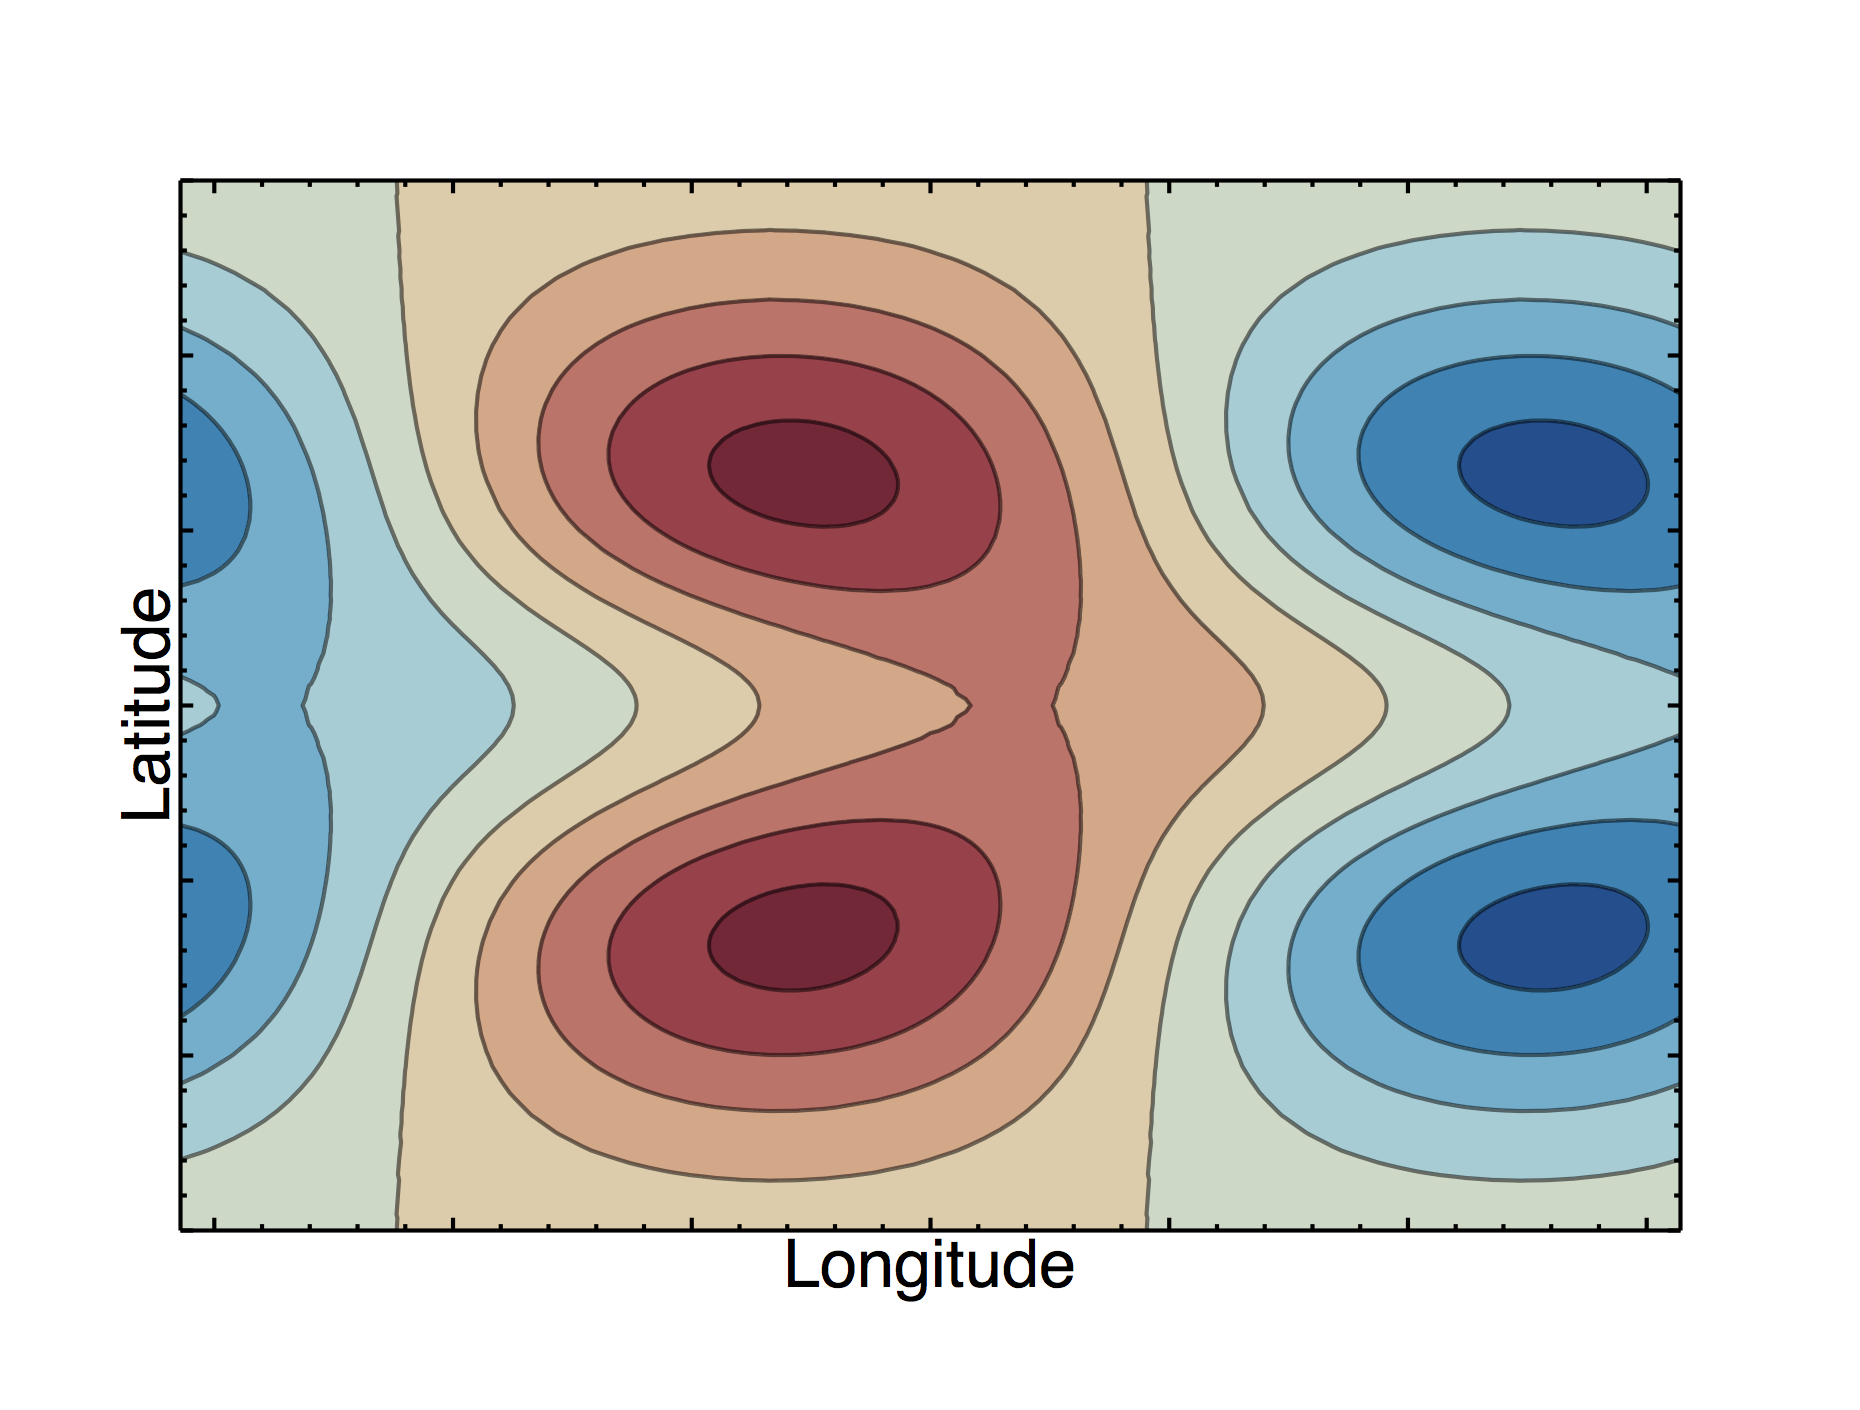
\includegraphics[width=\textwidth]{figures/wave-mean-flow/expl-non-shifted-matsuno.png}
    \caption{Zero background flow, $\overline{U}(y) = 0$. }
    \label{fig:expl-non-shifted-matsuno}
  \end{subfigure}
  %
  \begin{subfigure}[t]{0.48\textwidth}
    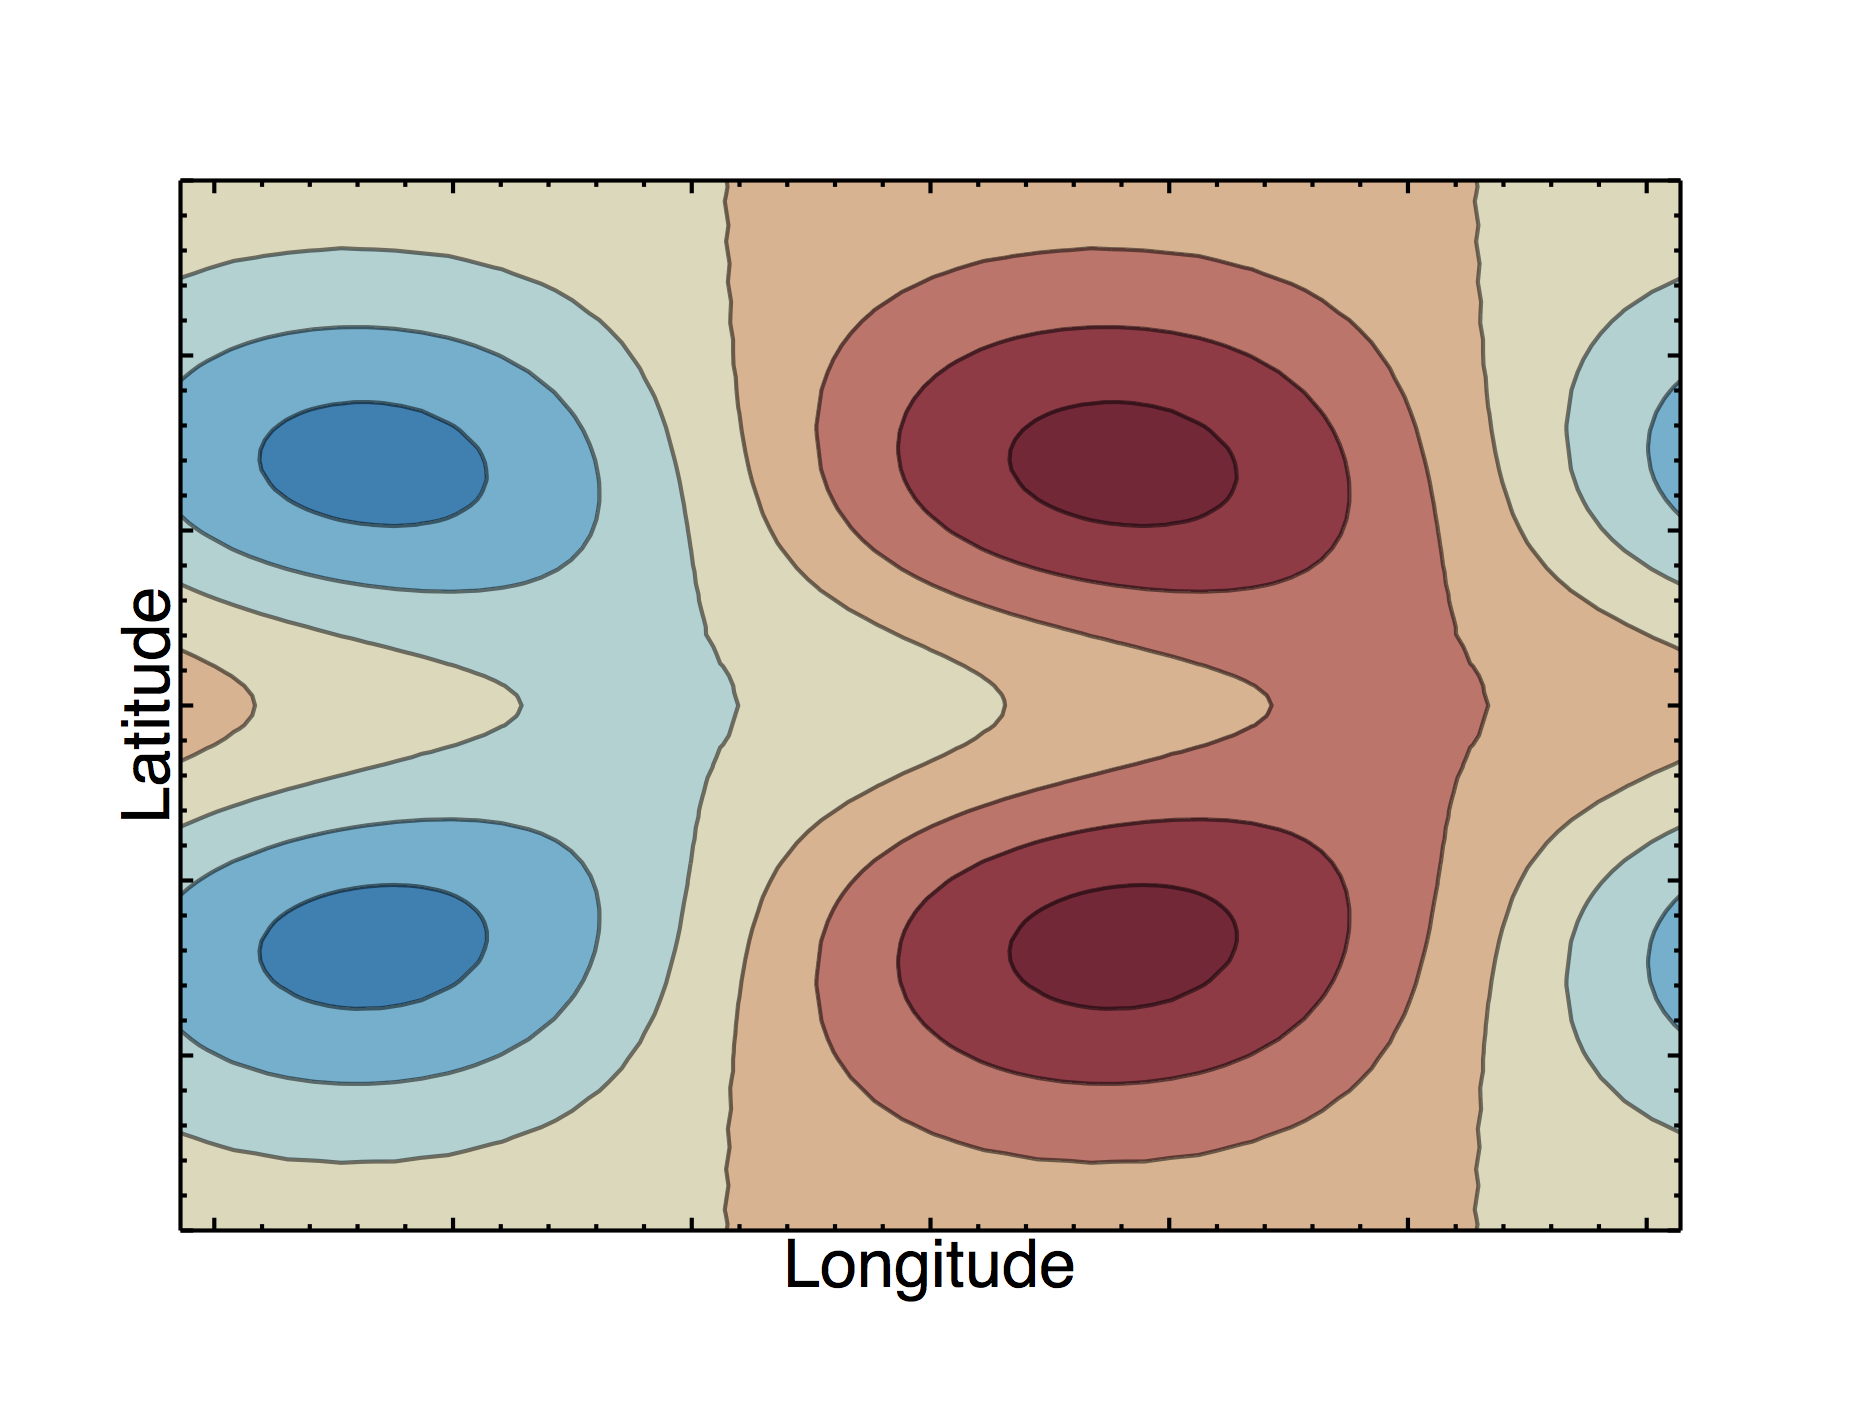
\includegraphics[width=\textwidth]{figures/wave-mean-flow/expl-shifted-matsuno.png}
    \caption{Uniform background flow, $\overline{U}(y) = \overline{U}_{0}$.}
    \label{fig:expl-shifted-matsuno}
  \end{subfigure}
\\
  \begin{subfigure}[t]{0.48\textwidth}
    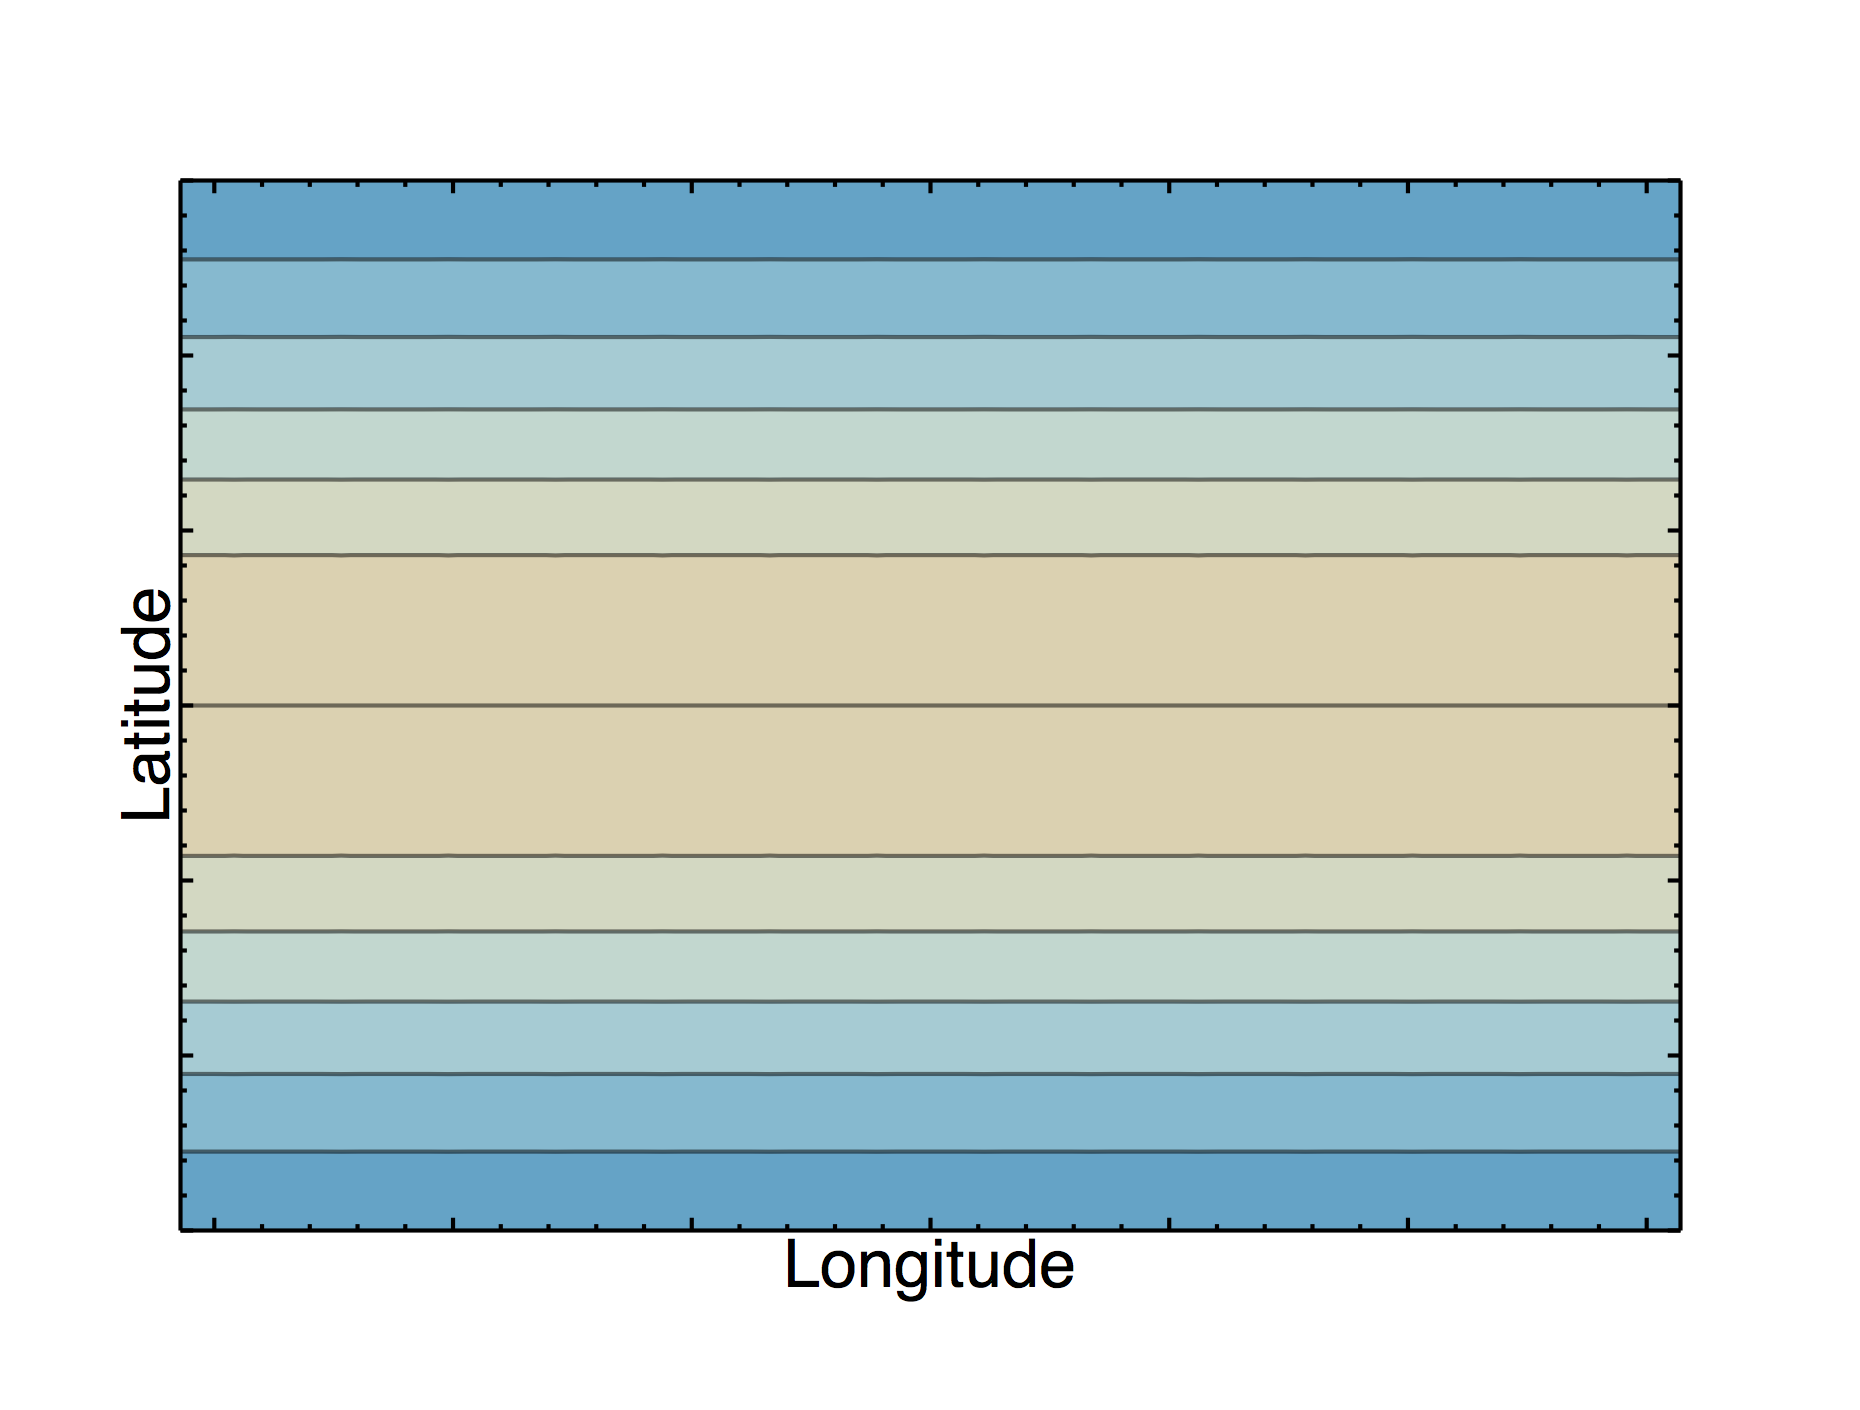
\includegraphics[width=\textwidth]{figures/wave-mean-flow/expl-phibar.png}
    \caption{Height field $\overline{H}(y)$ balancing $\overline{U}_{0}$.}
    \label{fig:expl-phibar}
  \end{subfigure}
  %
  \begin{subfigure}[t]{0.48\textwidth}
    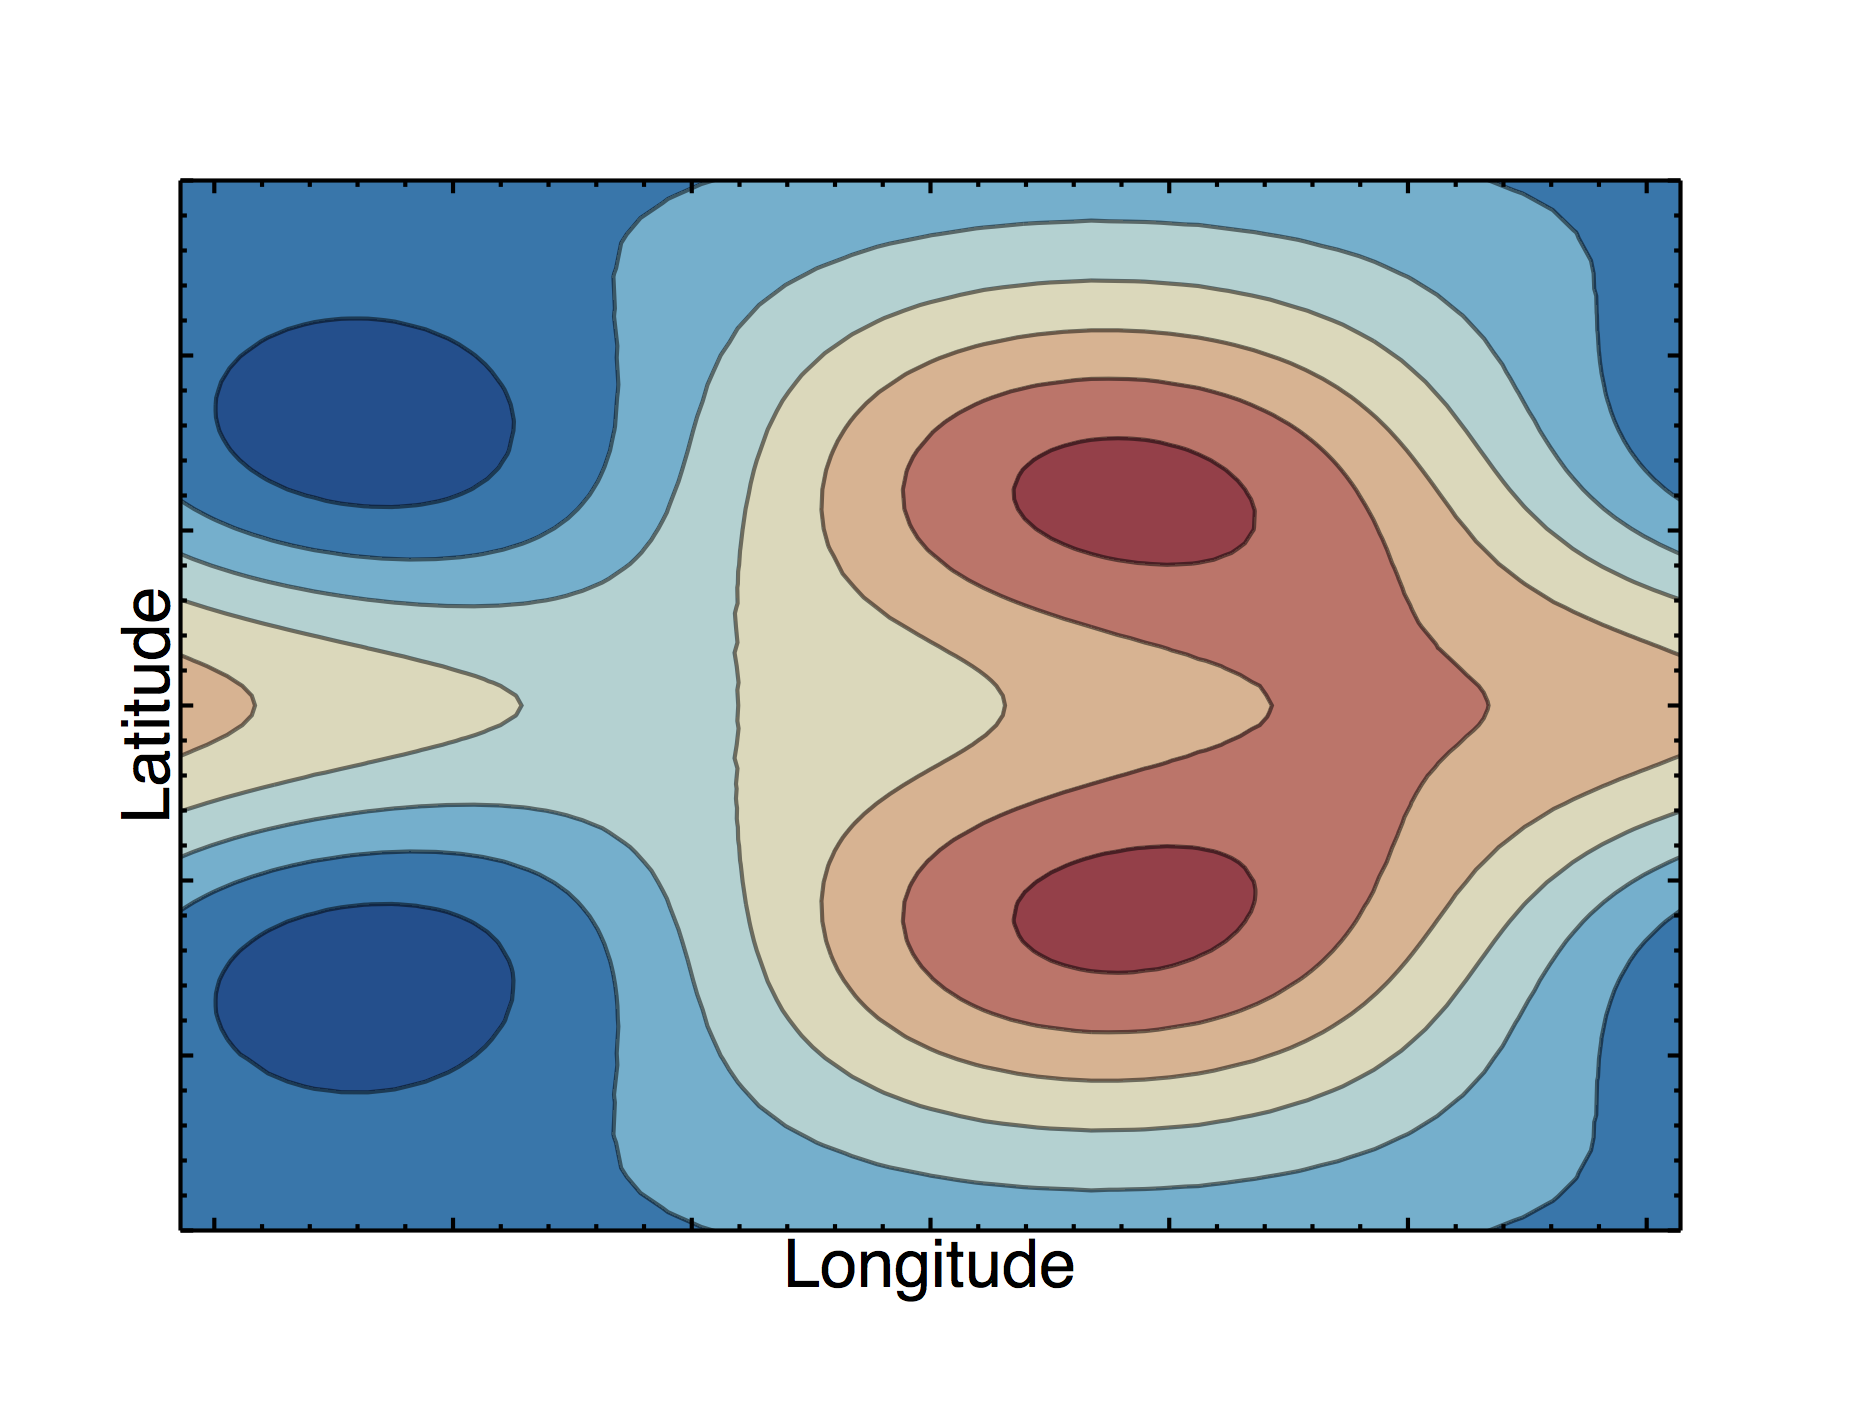
\includegraphics[width=\textwidth]{figures/wave-mean-flow/expl-plot-total.png}
    \caption{Sum of panels (b) and (c).}
    \label{fig:expl-plot-total}
  \end{subfigure}
  \caption{Height fields of various responses to forcing, showing how the sum of the Doppler-shifted height field and the height field due to the zonal jet produces the distinctive pattern in Figures \ref{fig:example-gcm-results} and \ref{fig:ps-flow}.}
  \label{fig:first-order-solutions}
\end{figure}

I have shown that the shallow-water response to forcing in a shear flow $\overline{U}(y)$ qualitatively matches a GCM simulation of a tidally locked planet. This section shows how the flow modifies the global circulation.

Figure \ref{fig:first-order-solutions} explains how the solution in a shear flow is built up from two main effects. The first panel shows the response to forcing in zero flow, with the same solution as \citet{matsuno1966quasi}. The second panel shows the response to forcing in a uniform flow $U_{0}$ (the same as the last panel of Figure \ref{fig:U0-shift-demo}). This flow shifts the Rossby and Kelvin modes eastwards, as explained in Section \ref{sec:shear-flow-beta-plane} \citep{tsai2014three}. The third panel shows the zonally uniform height perturbation $\overline{H}(y)$ that geostrophically balances the zonal flow.

The fourth panel shows the sum of the second and third panels. East of the substellar point, the on-equator maximum and off-equator maxima combine to form a large, meridionally continuous ``hot-spot''. West of the substellar point, the equatorial maximum and off-equator minima combine to increase the meridional height gradient. This preserves the off-equator cold Rossby lobes, unlike on the day-side where the hot Rossby lobes are subsumed into the hot-spot. Both of these features are in the same place as in the GCM simulations in Figure \ref{fig:example-gcm-results}.

This combination of effects also explains the velocities in Figure \ref{fig:example-gcm-results}. On the equator west of the substellar point, the eastward Rossby wave velocities combine with the eastward zonal jet to give strong eastward flow. East of the substellar point, the westward Rossby wave velocities on the equator oppose the jet, leading to the region of weak zonal flow east of the substellar point in Figure \ref{fig:example-gcm-results}. This simple model of the global circulation as the sum of the wave-0 jet and the wave-1 forced response will be used later to show how the observable temperature distribution scales with planetary parameters.




%
% What is the relevance of these forced solutions for the atmospheres of tidally locked planets, and interpreting observations of them?
%
% It is possible to match up the shifted eigenvalues of the free modes in Section X to the total forced response in Section X to understand the change in global temperature structure produced by the equatorial jet.

%SECTION CONCLUSIONS



%%%%%%%%%%%%%%%%%%%%%%%%%%%%%%%%%%%%
%SECTION 4 -- SHEAR FLOW IN SPHERICAL
\section{Forced Response in Shear Flow on a Sphere}\label{sec:shear-flow-sphere}

The forced linear system on a beta-plane is useful for an intuitive understanding of the wave-mean flow interactions, as it is closely linked to the simple analytic equatorial wave solutions of \citet{matsuno1966quasi}. The beta-plane is less useful for direct comparison with real planets or GCM simulations, as the assumption of a linear Coriolis parameter is inaccurate at high latitudes. It also does not directly represent the latitudinal direction or the effect of rotation rate, as the y-coordinate is non-dimensionalised to the equatorial Rossby radius. The system is therefore only appropriate for tidally locked planets where this radius is similar to the planetary radius.

This section shows the response to forcing for a shallow-water system in a spherical geometry. This represents the same physical system as the earlier beta-plane model, but is more directly comparable to GCM simulations, as it does not require that the equatorial Rossby radius is comparable to the planetary radius.

The shallow-water equations on a sphere, linearised about a zonally uniform background flow $\overline{U}(\phi)$ and height $\overline{H}(\phi)$ are \citep{dunkerton1990laplace, iga2005spherical}:

% original
% \begin{equation}\label{eqn:spherical-sw-eqns}
%   \begin{aligned}
%     {\frac{\partial u^{\prime}}{\partial t}+\frac{\partial\left(\overline{U} u^{\prime}\right)}{a \cos \theta \partial \lambda}+v^{\prime} \frac{\partial \overline{U}}{a \partial \theta}-\frac{\overline{U} v^{\prime} \tan \theta}{a}=2 \Omega v^{\prime} \sin \theta-\frac{g \partial h^{\prime}}{a \cos \theta \partial \lambda}}, \\
%      {\frac{\partial v^{\prime}}{\partial t}+\frac{\partial\left(\overline{U} v^{\prime}\right)}{a \cos \theta \partial \lambda}+\frac{2 \overline{U} u^{\prime} \tan \theta}{a}=-2 \Omega u^{\prime} \sin \theta-\frac{g \partial h^{\prime}}{a \partial \theta}}, \\
%      {\frac{\partial h^{\prime}}{\partial t}+v^{\prime} \frac{\partial \overline{H}}{a \partial \theta}+\overline{U} \frac{\partial h^{\prime}}{a \cos \theta \partial \lambda}+\overline{H} \nabla \cdot \mathbf{v}^{\prime}=F},
%   \end{aligned}
% \end{equation}

\begin{equation}\label{eqn:spherical-sw-eqns}
  \begin{aligned}
    {\frac{\partial u^{\prime}}{\partial t}+\frac{\partial\left(\overline{U} u^{\prime}\right)}{a \cos \theta \partial \lambda}+v^{\prime} \frac{\partial \overline{U}}{a \partial \theta}-\frac{\overline{U} v^{\prime} \tan \theta}{a}=2 \Omega v^{\prime} \sin \theta-\frac{g \partial h^{\prime}}{a \cos \theta \partial \lambda}}, \\
     {\frac{\partial v^{\prime}}{\partial t}+\frac{\partial\left(\overline{U} v^{\prime}\right)}{a \cos \theta \partial \lambda}+\frac{2 \overline{U} u^{\prime} \tan \theta}{a}=-2 \Omega u^{\prime} \sin \theta-\frac{g \partial h^{\prime}}{a \partial \theta}}, \\
     {\frac{\partial h^{\prime}}{\partial t}+v^{\prime} \frac{\partial \overline{H}}{a \partial \theta}+\overline{U} \frac{\partial h^{\prime}}{a \cos \theta \partial \lambda}+\overline{H} \nabla_{H} \cdot \mathbf{v}^{\prime}=0},
  \end{aligned}
\end{equation}

where $h$ is the height of the layer, $\boldsymbol{v} = (u,v)$ is the velocity, $\theta$ is latitude, $\lambda$ is longitude, $t$ is time, $a$ is radius, $g$ is gravity, and $\Omega$ is angular velocity. The forcing due to the day-night instellation is $F = F_{0} \cos \theta \sin \lambda$. Overbars denote zonal-mean quantities, which are the background zonal flow and the associated height field, and dashes denote perturbations to this background state.

The background state is stationary and in gradient wind balance, satisfying the meridional momentum equation in Equation \ref{eqn:spherical-sw-eqns}, which gives a different condition to the background height on the beta-plane:

\begin{equation}\label{eqn:gradient-wind-balance}
  \frac{1}{a} \frac{\partial}{\partial \theta}\left(\overline{H}+h_{g}\right)=-\left(2 \Omega \overline{U} \sin \theta+\frac{\overline{U}^{2}}{a} \tan \theta\right).
\end{equation}

The perturbed variables are wavelike in longitude and are uniformly damped, so are proportional to $e ^{i (m \lambda-\sigma t)}$, where $\sigma = i \alpha$. All variables are non-dimensionalised with velocity scale $2 \Omega a$, height scale $(2 \Omega a)^{2}/g$ and time scale $1/(2\Omega)$, and denoted as such by an asterisk. This gives the following non-dimensional shallow-water equations:

\begin{equation}\label{spherical-sw-eqns-nondim}
  \begin{aligned}
    \alpha^{*} u_{m}^{*}+i m \frac{\overline{U}^{*} u_{m}^{*}}{\cos \theta}+v_{m}^{*} \frac{\partial \overline{U}^{*}}{\partial \theta}-\overline{U}^{*} v_{m}^{*} \tan \theta &=v_{m}^{*} \sin \theta-\frac{i m h_{m}^{*}}{\cos \theta}, \\
    \alpha^{*} v_{m}^{*}+i m \frac{\overline{U}^{*} v_{m}^{*}}{\cos \theta}+2 \overline{U}^{*} u_{m}^{*} \tan \theta &=-u_{m}^{*} \sin \theta-\frac{\partial h_{m}^{*}}{\partial \theta}, \\
    \alpha^{*} h_{m}^{*}+i m \overline{U}^{*} \frac{h_{m}^{*}}{\cos \theta} &=-\frac{\epsilon^{*}}{\cos \theta}\left[i m u_{m}^{*}+\frac{\partial}{\partial \theta}\left(\cos \theta v_{m}^{*}\right)\right],
  \end{aligned}
\end{equation}

where $\epsilon \equiv(2 \Omega a)^{2} / g H$ is Lamb's parameter, which in this system determines the strength of the effect of the rotation of the planet \citep{longuet1968tidal}. This parameter was not present in the beta-plane system, where the effect of the rotation rate on the system was non-dimensionalised out by setting the meridional coordinate to the equatorial Rossby radius. I will show the effect of varying the rotation rate later in this section.

Appendix \ref{ap:ps-methods} shows how these coupled equations can be combined into a version of Laplace's tidal equation for the variable $\mu = \sin \theta$ \citep{dunkerton1990laplace}, modified to include the effect of the background shear flow:

\begin{equation}\label{eqn:tidal-eqn-U}
  \frac{\partial^{2} \phi_{m}^{*}}{\partial \mu^{2}}-B\left(\sigma^{*}, \mu\right) \frac{\partial \phi_{m}^{*}}{\partial \mu}-A\left(\sigma^{*}, \mu\right) \phi_{m}^{*}=\frac{F(\theta,x)}{i \sigma},
\end{equation}

where

\begin{equation}
  \begin{aligned} A\left(\sigma^{*}, \mu\right) \equiv & \frac{1}{1-\mu^{2}}\left[m(m+1)-m \mu \frac{1}{\Delta^{*}} \frac{\partial \Delta^{*}}{\partial \mu}+\epsilon \Delta^{*}\right.\\
  &+\frac{m}{\Delta^{*} \hat{\sigma}^{*}}\left(f_{1}^{*} \frac{\partial \Delta^{*}}{\partial \mu}-\Delta * \frac{\partial f_{1}^{*}}{\partial \mu}\right) ], \\
  B\left(\sigma^{*}, \mu\right) & \equiv \frac{1}{\Delta^{*}} \frac{\partial \Delta^{*}}{\partial \mu}+\frac{2 \mu(m+1)}{\left(1-\mu^{2}\right)}, \\ \Delta^{*} & \equiv f_{1}^{*} \overline{\zeta}^{*}-\hat{\sigma}^{* 2}.
 \end{aligned}
\end{equation}

% %SUBSECTION --
% \subsection{Solution to the Forced Tidal Equations}

Appendix \ref{ap:ps-methods} shows how Equation \ref{eqn:tidal-eqn-U} is solved with the Chebyshev pseudo-spectral collocation method used in \citet{wang2016hough} to find the eigenfunctions of Laplace's tidal equation on a sphere \citep{longuet1968tidal, dunkerton1990laplace}.

The free parameters of the system are the forcing strength $F_{0}$, damping rate $\alpha$, rotation rate $\Omega$, radius $a$, gravity $g$, and background height $H_{0}$. The background flow is set by the jet speed $U_{0}$ and jet width $L_{jet}$, for a flow profile $\overline{U} = U_{0} \exp(-\mu^{2}/L_{jet}) \cos \theta$ where $\mu = \sin \theta$. The default parameters of $F_{0} = 0.3$, $\alpha = 0.6$, $\Omega = 1.0$, $a = 1.0$, $g = 2.0$, $H_{0} = 1.0$, $U_{0} = 0.75$, and $L_{jet} = \sqrt{3}$ were based on the GCM simulation in Figure \ref{fig:example-gcm-results}.

Figure \ref{fig:spherical-solutions} shows the effect of the background zonal flow $\overline{U}$ on the response to day-night forcing in a spherical geometry. The background flow Doppler-shifts the maximum of the wave response eastwards, as was the case in Figure \ref{fig:ps-flow} on the beta-plane, and adds a zonally uniform height perturbation centred on the equator. The resulting response to forcing is qualitatively similar to the simulation in Figure \ref{fig:example-gcm-results}.


\begin{figure}
  \centering
  \begin{subfigure}[t]{0.48\textwidth}
    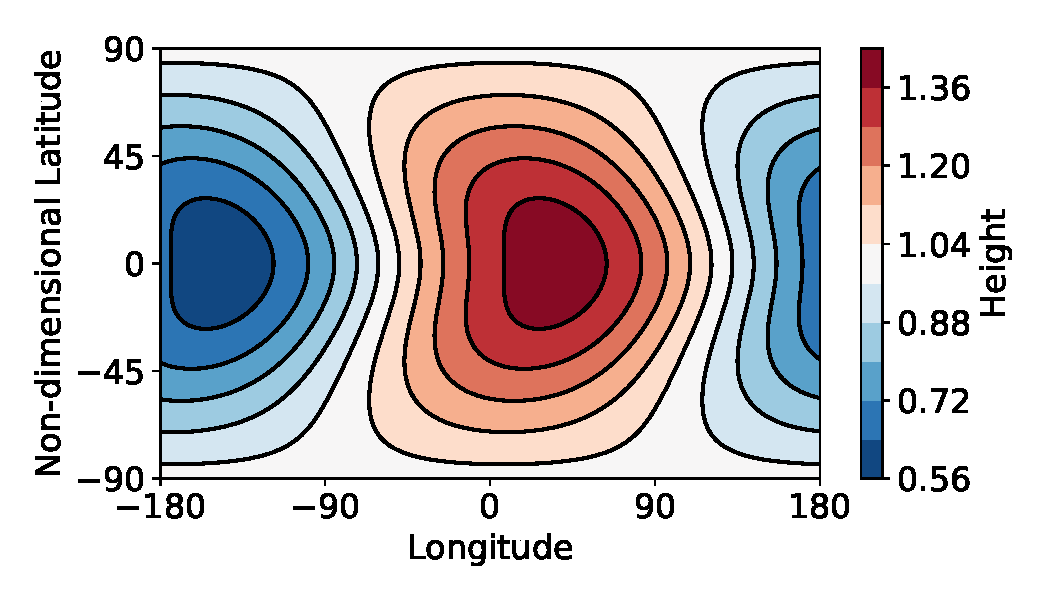
\includegraphics[width=\textwidth]{figures/wave-mean-flow/new-sphere-non-shifted.pdf}
    \caption{The forced solution with zero background flow, similar to the beta-plane solution in \citet{matsuno1966quasi} .}
    \label{fig:non-shifted-sphere}
  \end{subfigure}
\quad
  \begin{subfigure}[t]{0.48\textwidth}
    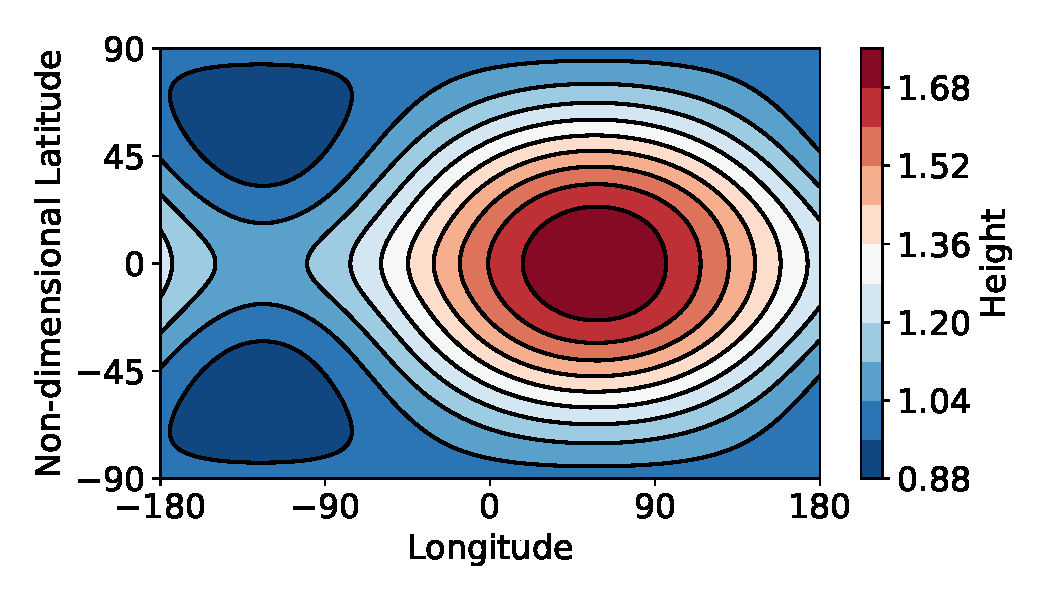
\includegraphics[width=\textwidth]{figures/wave-mean-flow/new-sphere-shifted.pdf}
    \caption{The forced solution with background flow $U_{0} \exp(-\mu^{2}/L_{jet}) \cos \theta$, $U_{0}=0.75$, matching the simulations in Figure \ref{fig:example-gcm-results}.}
    \label{fig:shifted-sphere}
  \end{subfigure}
  \caption{The effect of a background shear flow $\overline{U}(\phi)$ on the forced solutions of Equation \ref{eqn:spherical-sw-eqns}, matching the form of the beta-plane solutions in Figure \ref{fig:ps-flow}.}
  \label{fig:spherical-solutions}
\end{figure}


%SECTION CONCLUSIONS



%%%%%%%%%%%%%%%%%%%%%%%%%%%%%%%%%%%%

%SECTION 5 -- SCALING RELATIONS
\section{Scaling Relations}\label{sec:sw-scaling-relations}

The previous section showed how the global circulation on a tidally locked planet is a combination of a wave-0 jet and a wave-1 response to day-night forcing. This section considers how each of these components depend on planetary parameters, to predict how the global circulation and temperature distribution scales with these parameters. \citet{komacek2016daynightI} and \citet{zhang2017dynamics} produced 1D scaling relations based on a balance of advective and radiative timescales on the equator to predict how observables such as hot-spot shift and day-night contrast scale with planetary parameters. This section derives similar 1D scaling relations using the shallow-water model, discusses the 2D scaling of the global circulation, and compares these predictions to GCM simulations.

%SUBSECTION -- 1D SCALING
\subsection{1D Scaling Relations}\label{sec:1d-scaling}

Reducing the 2D shallow-water system to a 1D system on the equator gives an analytically solvable system, which provides simple predictions of the observable hot-spot shift and day-night contrast. Setting $\phi = 0$ and retaining only the damping and advection terms, the third line of Equation \ref{eqn:shear-sw-equations},

\begin{equation}
      \frac{\partial \overline{H}' u}{\partial x} + \overline{H}'\frac{\partial v}{\partial y} - y\overline{U}(y) v +\frac{\partial h}{\partial t} +  \alpha_{rad} h + \frac{\partial \overline{U}(y) h}{\partial x} = Q(y),
\end{equation}

becomes

\begin{equation}
   \frac { \partial  h  } { \partial t } + \alpha h + \frac { \partial  U_{0} h } { \partial x } = Q_{0}.
\end{equation}

The stationary wave-1 response is found by setting $\partial/ \partial t = 0 $ and $\partial/ \partial x =i k_{x}$:

\begin{equation}\label{eqn:on-equator-height}
-\alpha h (y=0) + i k_{x} { U }_{0} h (y=0) = Q_{0}.
\end{equation}

So, the on-equator height perturbation $h (x,y=0)=h (y=0)e^{i k_{x}x}$ is:

\begin{equation}\label{eqn:phi-curve}
  h (x,y=0)=\frac{Q_{0}}{\alpha^{2}+k_{x}^{2}U_{0}^{2}}(-\alpha \cos(k_{x}x)+k_{x}U_{0}\sin{k_{x}x}).
\end{equation}

This is a sinusoidal height perturbation on the equator, with magnitude

\begin{equation}\label{eqn:1d-scaling-hss}
  h_{0}=\frac{\alpha+k_{x}U_{0}}{\alpha^{2}+k_{x}^{2}U^{2}}Q_{0}.
\end{equation}

The hot-spot shift $x_{0}$ is at the maximum of this sinusoidal curve, where $\partial h / \partial x = 0$:

\begin{equation}\label{eqn:x0}
  x_{0}=\frac{1}{k_{x}}\tan^{-1}(k_{x}\frac{U_{0}}{\alpha}).
\end{equation}

This is the same as the simplest approximation of the hot-spot shift calculated by \citet{zhang2017dynamics}, $\lambda_{s}=\tan^{-1}(\frac{\tau_{rad}}{\tau_{adv}})$, (where $\tau_{rad}$ corresponds to $1/\alpha$ and $\tau_{adv}$ corresponds to $k_{x}/U_{0}$). Equation \ref{eqn:x0} predicts that the hot-spot shift varies between \ang{0} and \ang{90} east of the substellar point. There are two similar ways to interpret this physically. First, the size of the shift can be seen as a balance between the jet transporting heat eastwards according to the advective timescale $\tau_{adv}$, and the heat radiating away according to the radiative timescale $\tau_{rad}$ \citep{komacek2016daynightI, zhang2017dynamics, hammond2017climate}. Or, as discussed above, they can instead be seen as a balance of the flow $U_{0}$ shifting the stationary waves \ang{90} out of phase with the forcing, versus the damping $\alpha_{rad}$ bringing them in phase with the forcing \citep{tsai2014three, hammond2018wavemean}. Section \ref{sec:shift-mechanism} discusses these two mechanisms in more detail.


%SUBSECTION -- 2D SCALING
\subsection{2D Scaling Relations}\label{sec:2d-scaling}

% Varying the parameters of spherical shallow-water system shows their effect on the global circulation of the planet.

\begin{figure}
  \centering
  \begin{subfigure}[t]{0.48\textwidth}
    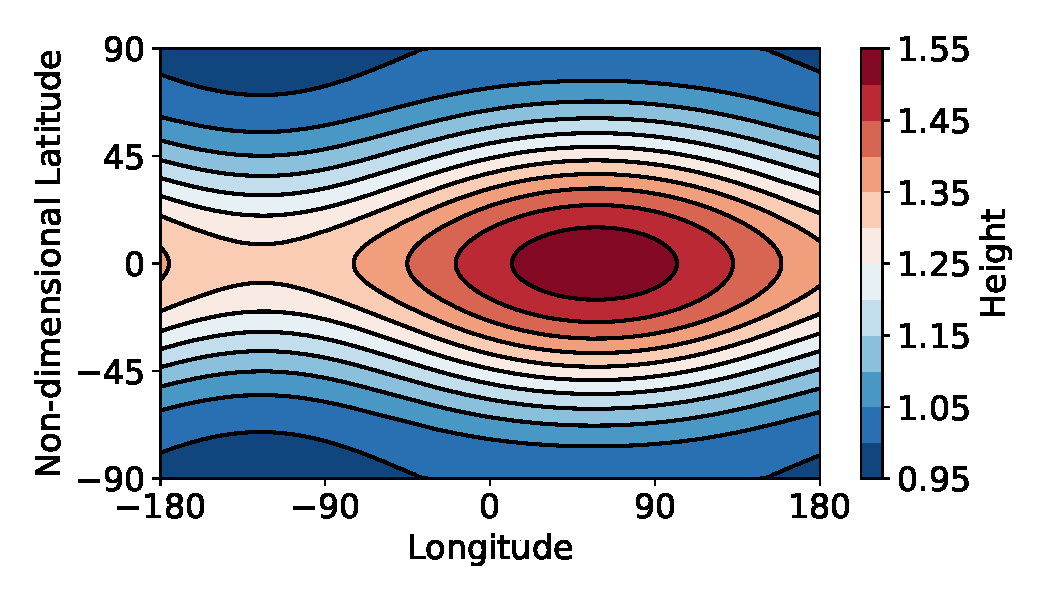
\includegraphics[width=\textwidth]{figures/wave-mean-flow/spherical-low-F.pdf}
    \caption{$F_{0} = 0.1$, giving a weak wave-1 component and  a more zonally uniform field.}
    \label{fig:spherical-low-F}
  \end{subfigure}
  \quad
  \begin{subfigure}[t]{0.48\textwidth}
    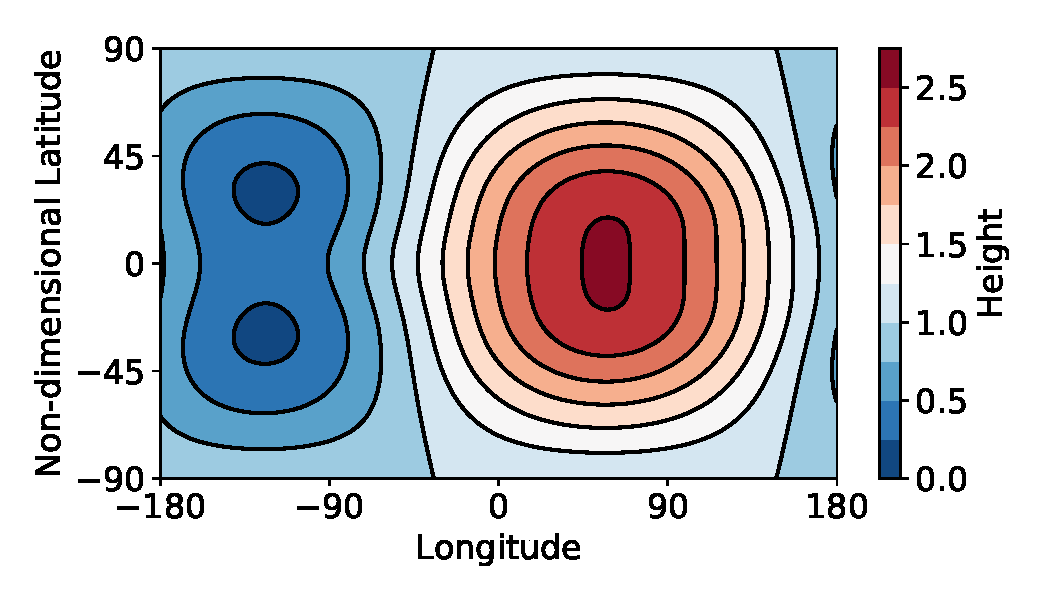
\includegraphics[width=\textwidth]{figures/wave-mean-flow/spherical-high-F.pdf}
    \caption{$F_{0} = 1.0$, giving a strong wave-1 component and a less zonally uniform field.}
    \label{fig:spherical-high-F}
  \end{subfigure}
  \caption{Spherical solutions with low and high forcing $F_{0}$, showing how this affects the strength of the wave-1 component relative to the unchanged wave-0 jet component, affecting the longitudinal variation and day-night contrast.}
  \label{fig:spherical-F-effect}
\end{figure}

This section shows how the forcing strength, damping rate, and rotation rate affect the global circulation in the linear shallow-water model on a sphere. The spherical shallow-water model is better suited to this than the beta-plane model, as it includes the effect of rotation rate. In the next section, I will show how this qualitatively explains the global circulation of a suite of GCM tests.

Figure \ref{fig:spherical-F-effect} shows the effect of varying the forcing magnitude $F_{0}$ in a system with all other parameters the same as those in Figure \ref{fig:shifted-sphere}. The case with low $F_{0}$ has a weak wave-1 height field due to the day-night forcing compared to its wave-0 height field due to the jet, so the global height field is very zonally uniform. In contrast, the case with high $F_{0}$ has a much stronger wave-1 height field so varies greatly with longitude. The hot-spot shifts are the same in both cases, as the Doppler-shift is not affected. If the atmosphere is in hydrostatic equilibrium, the height field corresponds to the temperature field, so is directly observable through the thermally emitted phase curve. The phase curve of the case with high $F_{0}$ would have a much larger magnitude than weakly forced case, but their phase shifts would be the same. Chapter \ref{ch:linking-climate-55cnce} investigates the behaviour of thermal phase curves in more detail for the planet 55 Cancri e.

Figure \ref{fig:spherical-damp-effect} shows the effect of varying the damping rate $\alpha$ in the same system. The case with low damping is similar to the case with high forcing, as it also increases the strength of the wave-1 field relative to the zonally uniform field. The case with high damping has a weak wave-1 response, and a smaller hot-spot shift as the high damping rate brings the maximum more closely into phase with the forcing. The weakly damped case would have a phase curve with a large amplitude and large phase shift, while the strongly damped case would have a small amplitude and a small phase shift.

Figure \ref{fig:spherical-omega-effect} shows the effect of the rotation rate $\Omega$. $\Omega$ scales the magnitude of the zonally uniform height perturbation due to the jet, due to the $f$ dependence in Equation \ref{eqn:gradient-wind-balance}. This means that $\Omega$ has the same leading-order effect as $F_{0}$, scaling the magnitude of the zonally uniform height perturbation relative to the wave-1 forced response. The case with low $\Omega$ would have a phase curve with a large amplitude and large phase shift, while the case with high $\Omega$ would have a smaller amplitude.




\begin{figure}
  \centering
  \begin{subfigure}[t]{0.48\textwidth}
    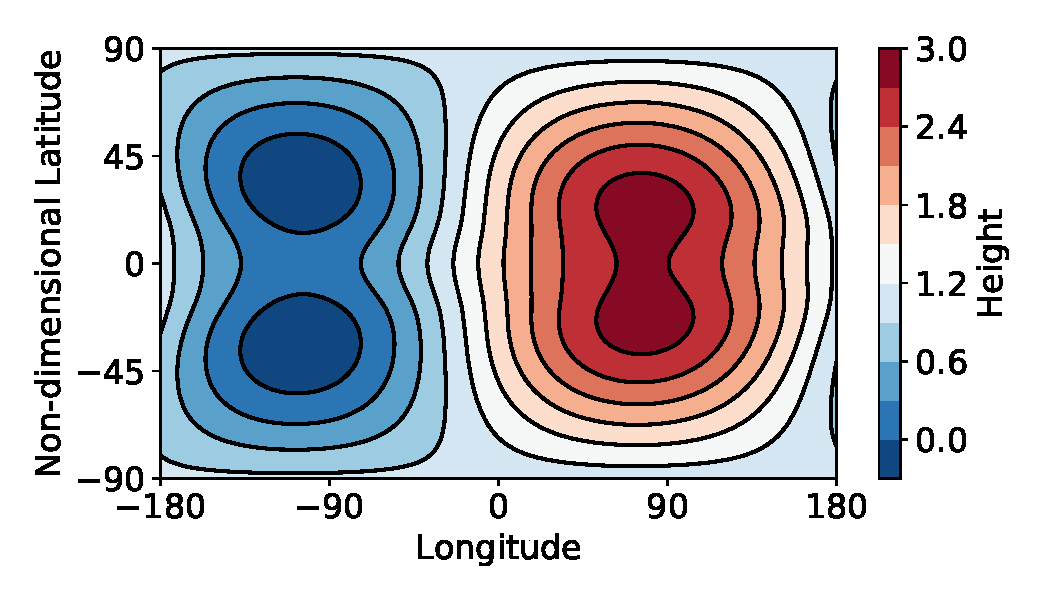
\includegraphics[width=\textwidth]{figures/wave-mean-flow/spherical-low-damp.pdf}
    \caption{$\alpha = 0.2$, giving a strong wave-1 component and a large hot-spot shift.}
    \label{fig:spherical-low-damp}
  \end{subfigure}
  \quad
  \begin{subfigure}[t]{0.48\textwidth}
    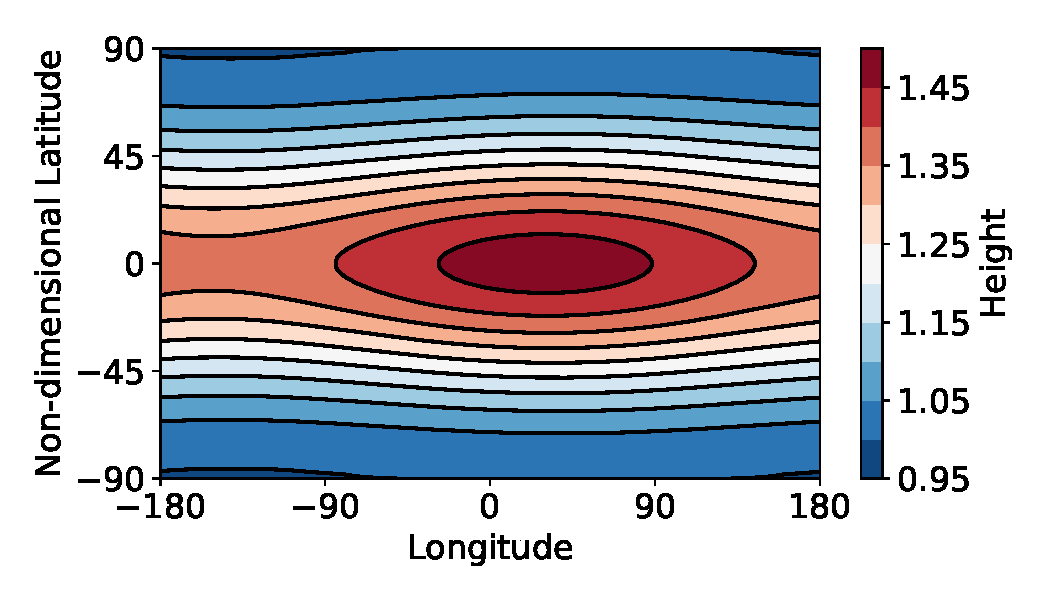
\includegraphics[width=\textwidth]{figures/wave-mean-flow/spherical-high-damp.pdf}
    \caption{$\alpha = 2.0$, giving a weak wave-1 component and a smaller hot-spot shift.}
    \label{fig:spherical-high-damp}
  \end{subfigure}
  \caption{Spherical solutions with low and high damping $\alpha$, showing how this affects the strength of the wave-1 component and the magnitude of the Doppler-shift of the wave components.}
  \label{fig:spherical-damp-effect}
\end{figure}


\begin{figure}
  \centering
  \begin{subfigure}[t]{0.48\textwidth}
    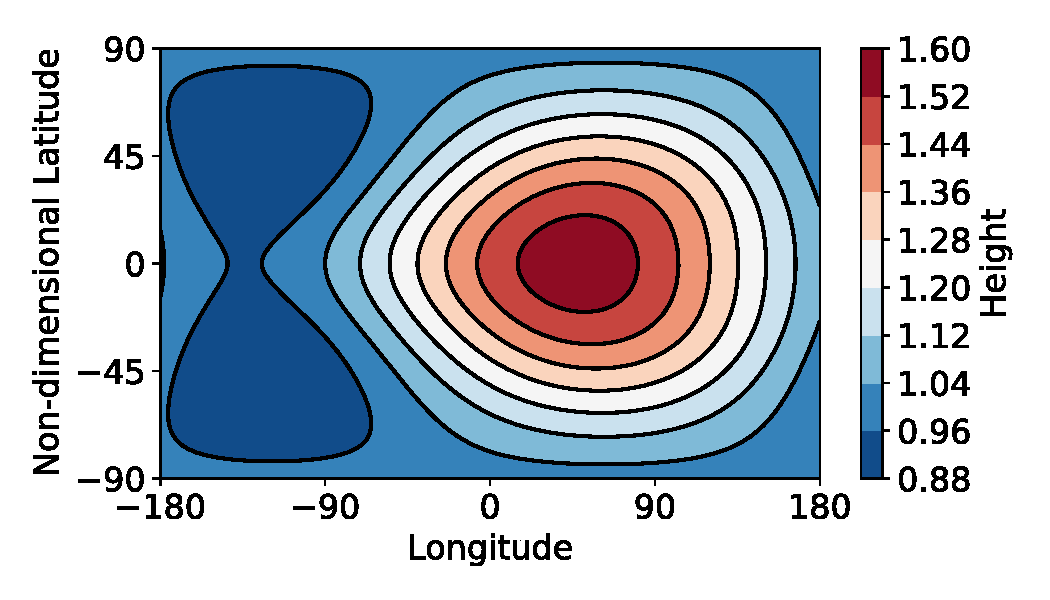
\includegraphics[width=\textwidth]{figures/wave-mean-flow/spherical-low-omega.pdf}
    \caption{$\Omega = 0.3$, giving a weak wave-0 component and a large day-night contrast.}
    \label{fig:spherical-low-omega}
  \end{subfigure}
  \quad
  \begin{subfigure}[t]{0.48\textwidth}
    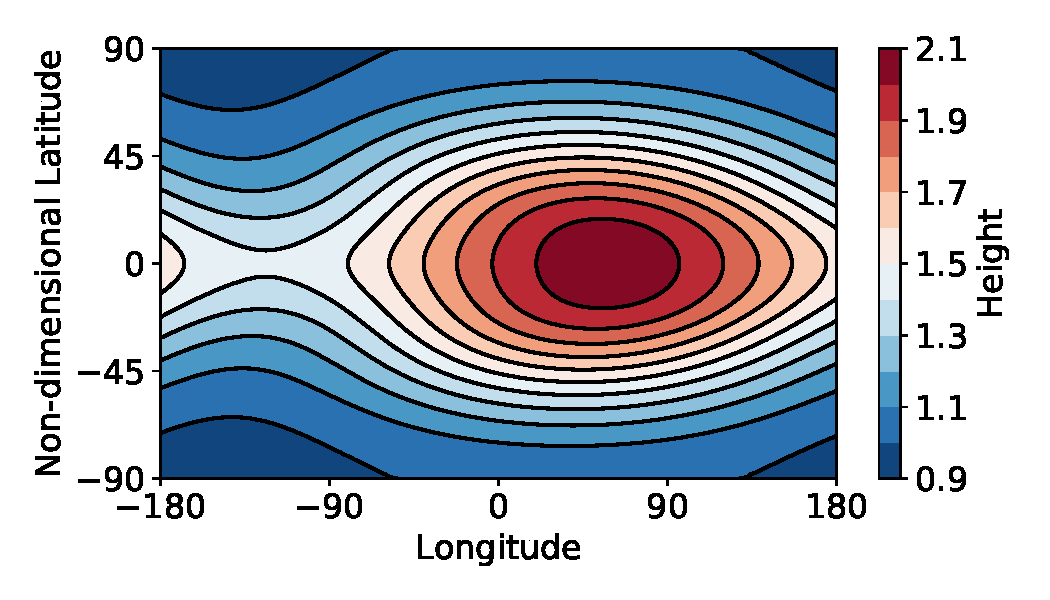
\includegraphics[width=\textwidth]{figures/wave-mean-flow/spherical-high-omega.pdf}
    \caption{$\Omega = 3.0$, giving a strong wave-0 component and a small day-night contrast.}
    \label{fig:spherical-high-omega}
  \end{subfigure}
  \caption{Spherical solutions with low and high rotation rate $\Omega$, showing how this affects the magnitude of the wave-0 height perturbation $\overline{H}(\phi)$ balancing the imposed shear flow $\overline{U}(\phi)$.}
  \label{fig:spherical-omega-effect}
\end{figure}

%SUBSECTION -- GCM SCALING
\subsection{GCM Scaling Relations}

These shallow-water solutions predict how the GCM should respond to changes in its input parameters. Figure \ref{fig:gcm-suite-temperature} shows a suite of tests in Exo-FMS that vary the instellation and rotation rate of the test plotted in Figure \ref{fig:example-gcm-results}. The instellation corresponds to the forcing strength in the shallow-water model, and also indirectly affects the radiative damping rate via the atmospheric equilibrium temperature.

Changing the forcing, damping, and rotation rate has the same qualitative effects in these GCM tests as in the shallow-water model. Increasing the forcing makes the atmospheres hotter, giving larger day-night temperature differences (matching the shallow-water solutions with high forcing). The colder tests are more zonally uniform, as their jets dominate the global height field. The more rapidly rotating tests are also more zonally uniform, as this increases the zonally uniform height perturbation of the jet, due to its dependence on $\Omega$ in Equation \ref{eqn:gradient-wind-balance}. This is especially clear in the ``cold'' tests, where the more rapidly rotating tests are very zonally uniform.

In the shallow-water model, an increased damping rate gave a smaller hot-spot shift, as it brought the wave response into phase with the forcing. In the GCM, the colder tests have a low damping rate so all have hot-spots shifted further east. The hotter tests have higher damping rates so have smaller hot-spot shifts -- this is especially clear in the 2 day cases. Chapter \ref{ch:linking-climate-55cnce} also shows the effect of damping, where varying the mean molecular weight of the atmosphere affects the damping rate and changes the hot-spot shift.


\begin{figure}
  \centering
  \begin{subfigure}[b]{0.32\textwidth}
    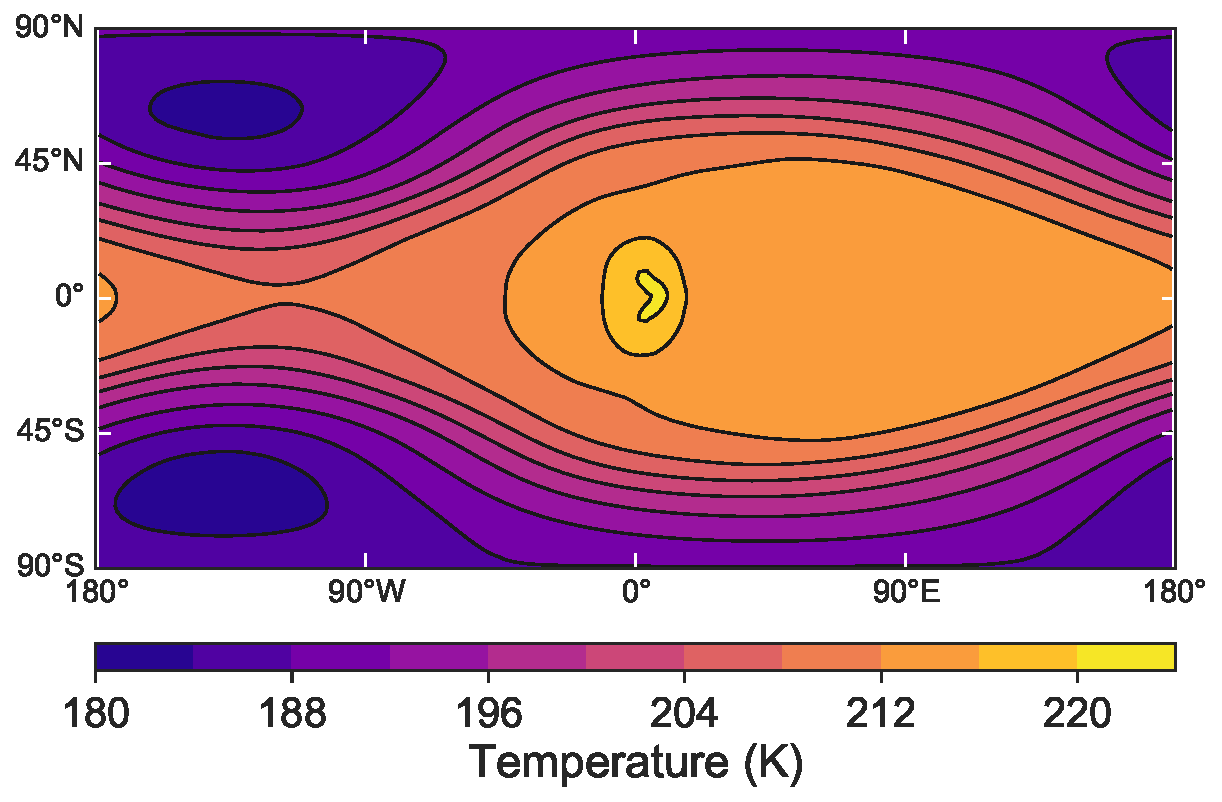
\includegraphics[width=\textwidth]{figures/wave-mean-flow/ar_lowT_10day.pdf}
    \caption{\SI{272}{\watt\per\metre\squared}, 10 days.}
    \label{fig:spherical-low-omega}
  \end{subfigure}
  \begin{subfigure}[b]{0.32\textwidth}
    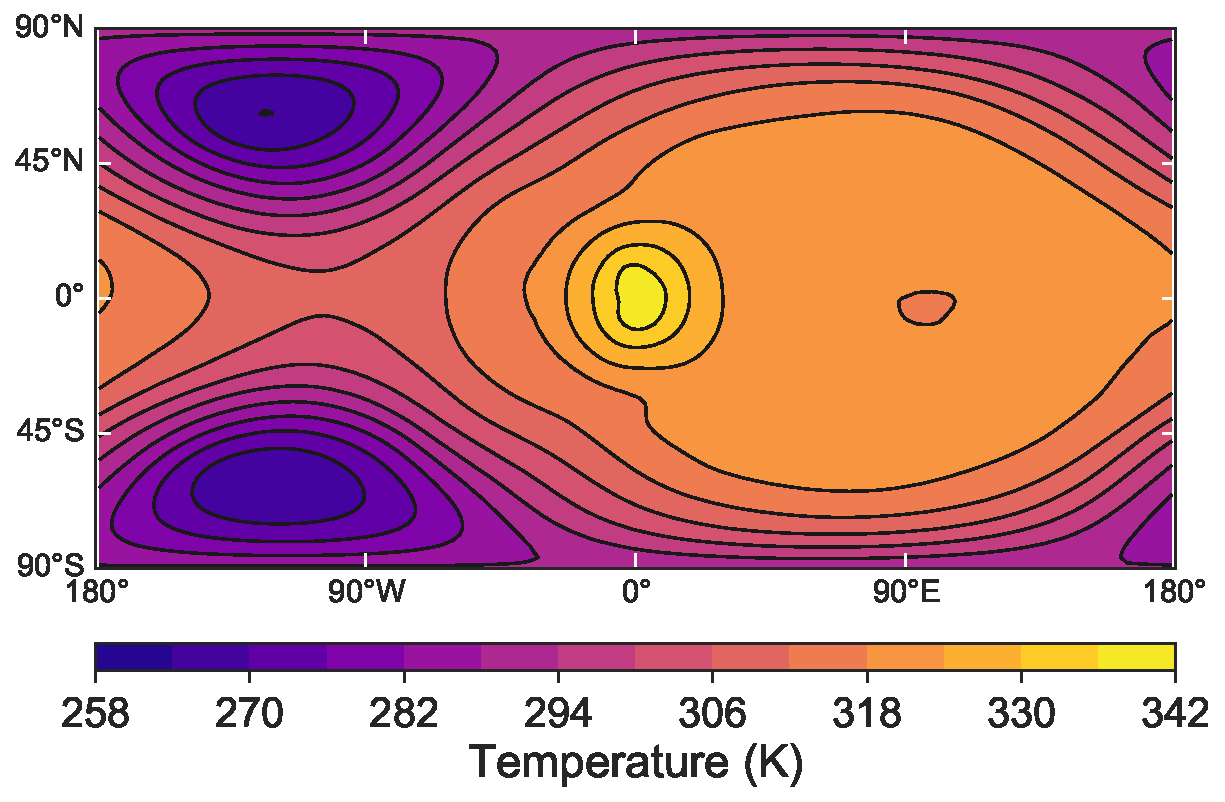
\includegraphics[width=\textwidth]{figures/wave-mean-flow/ar_mediumT_10day.pdf}
    \caption{\SI{1376}{\watt\per\metre\squared}, 10 days.}
    \label{fig:spherical-low-omega}
  \end{subfigure}
  \begin{subfigure}[b]{0.32\textwidth}
    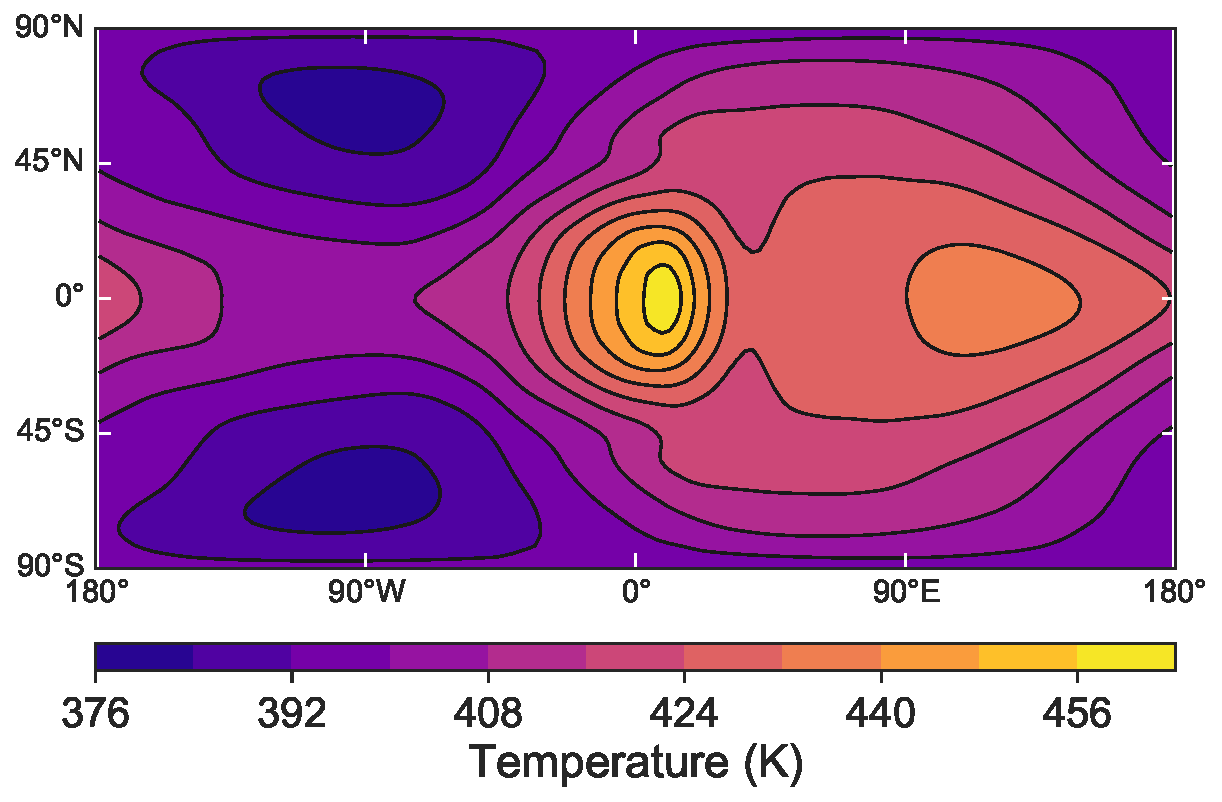
\includegraphics[width=\textwidth]{figures/wave-mean-flow/ar_highT_10day.pdf}
    \caption{\SI{4320}{\watt\per\metre\squared}, 10 days.}
    \label{fig:spherical-high-omega}
    \end{subfigure}
    \\
    \begin{subfigure}[b]{0.32\textwidth}
      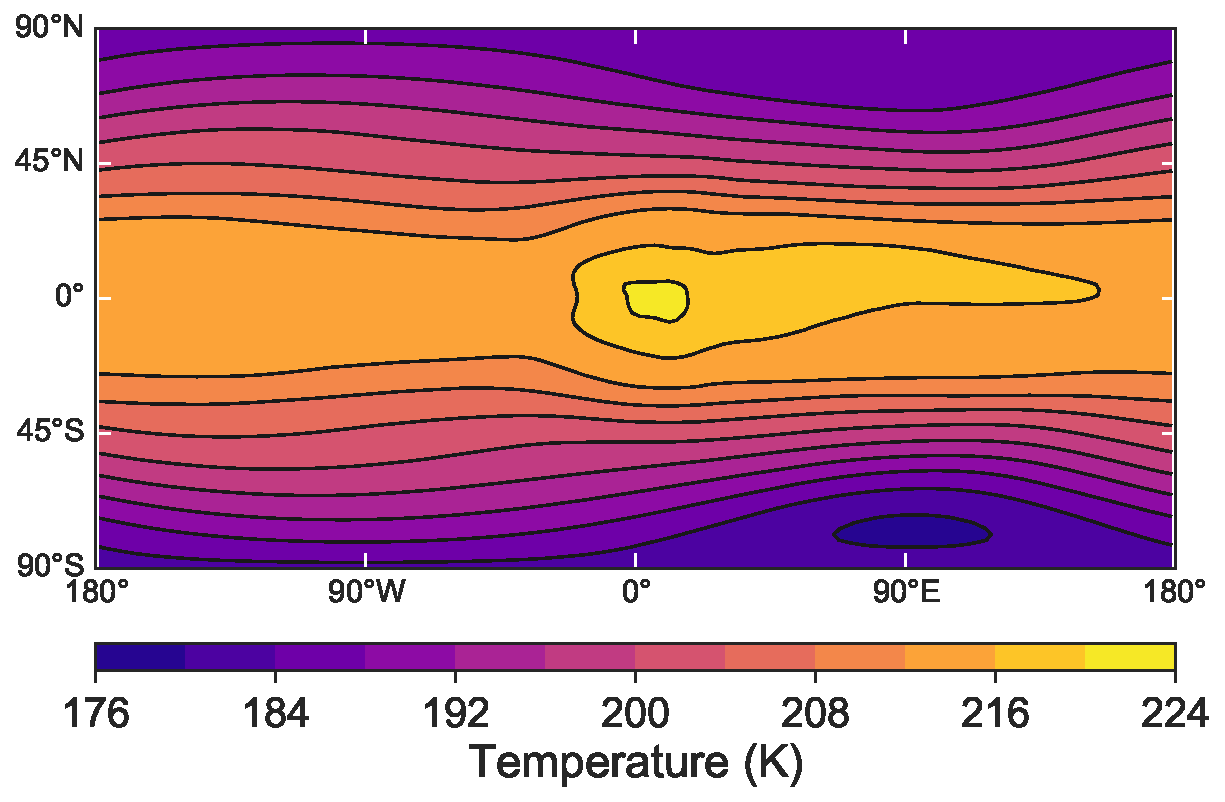
\includegraphics[width=\textwidth]{figures/wave-mean-flow/ar_lowT_5day.pdf}
    \caption{\SI{272}{\watt\per\metre\squared}, 5 days.}
      \label{fig:spherical-low-omega}
    \end{subfigure}
    \begin{subfigure}[b]{0.32\textwidth}
      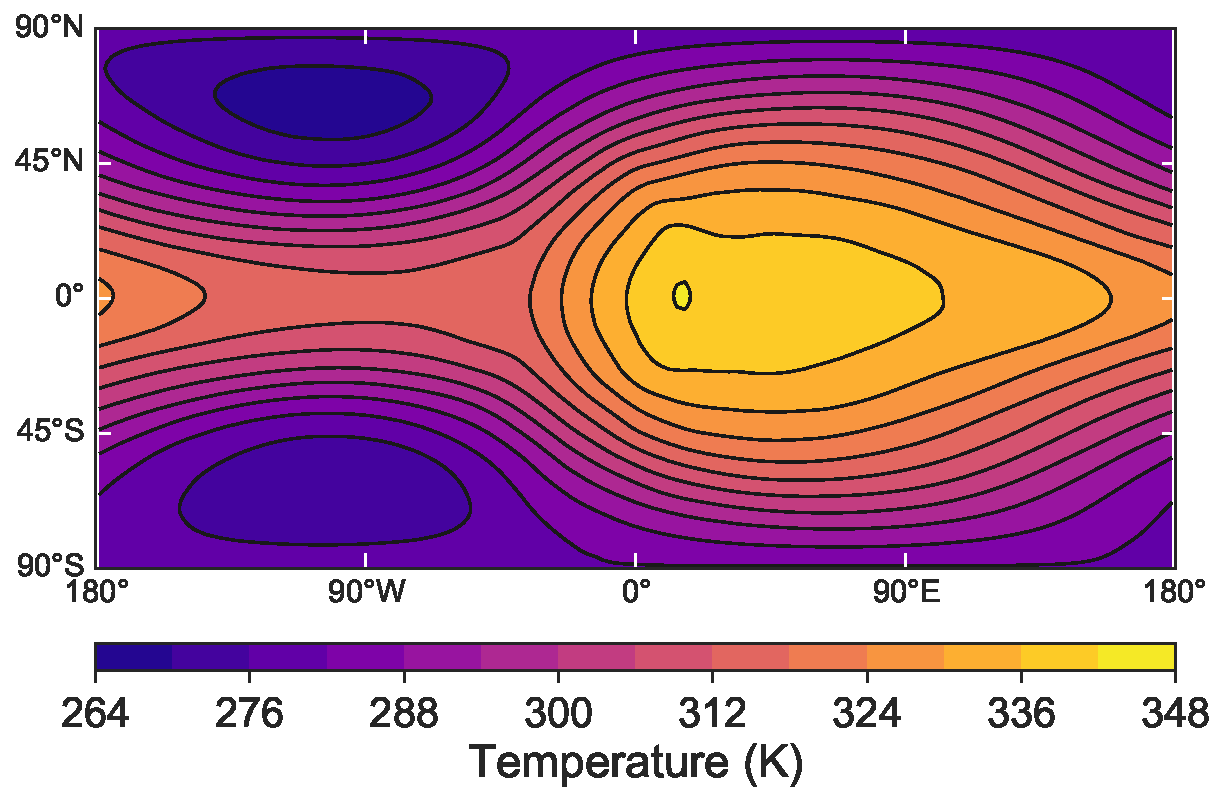
\includegraphics[width=\textwidth]{figures/wave-mean-flow/ar_mediumT_5day.pdf}
      \caption{\SI{1376}{\watt\per\metre\squared}, 5 days.}
      \label{fig:spherical-low-omega}
    \end{subfigure}
    \begin{subfigure}[b]{0.32\textwidth}
      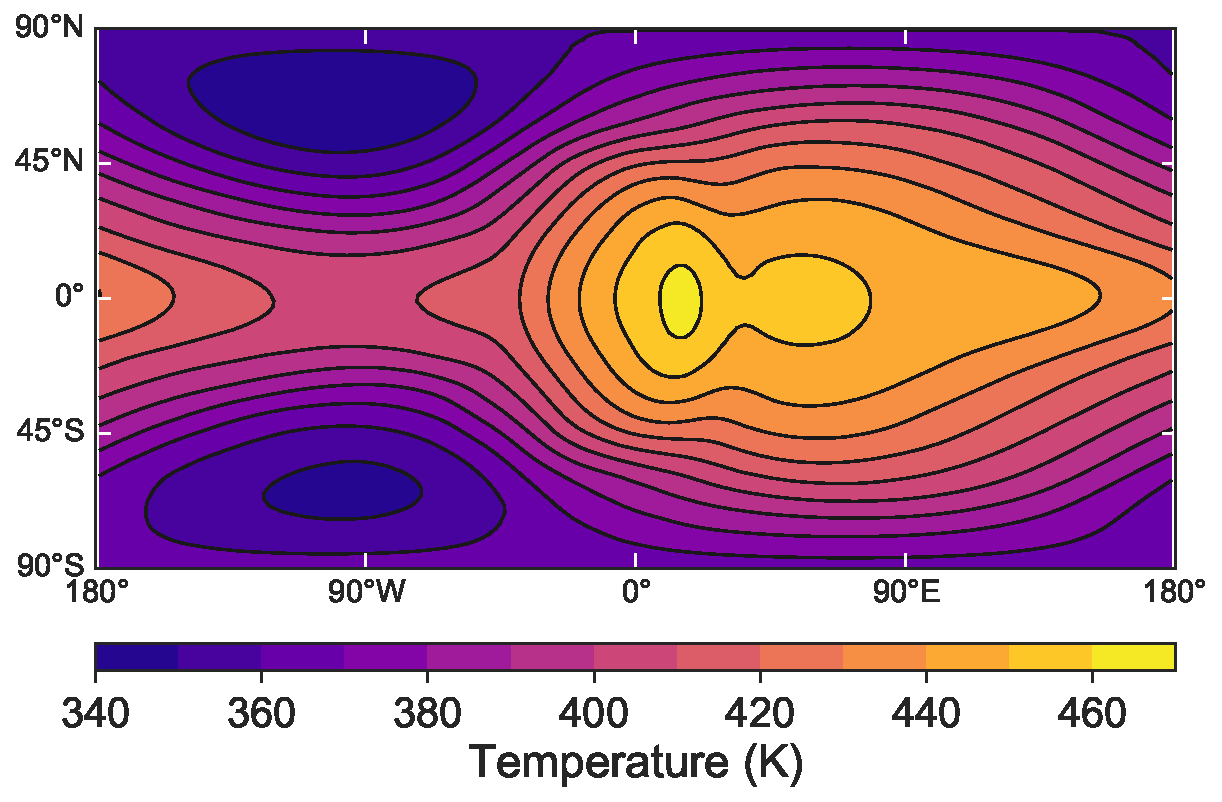
\includegraphics[width=\textwidth]{figures/wave-mean-flow/ar_highT_5day.pdf}
      \caption{\SI{4320}{\watt\per\metre\squared}, 5 days.}
      \label{fig:spherical-high-omega}
      \end{subfigure}
     \\
      \begin{subfigure}[b]{0.32\textwidth}
        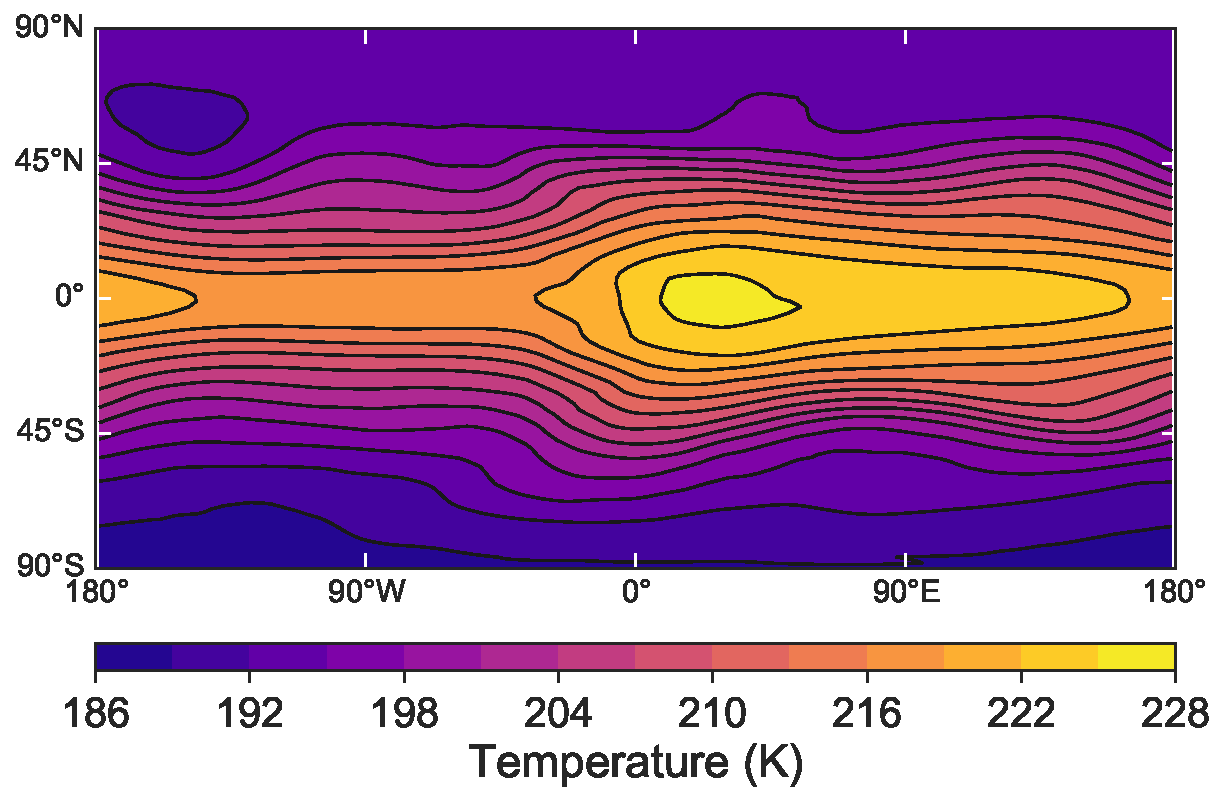
\includegraphics[width=\textwidth]{figures/wave-mean-flow/ar_lowT_2day.pdf}
        \caption{\SI{272}{\watt\per\metre\squared}, 2 days.}
        \label{fig:spherical-low-omega}
      \end{subfigure}
      \begin{subfigure}[b]{0.32\textwidth}
        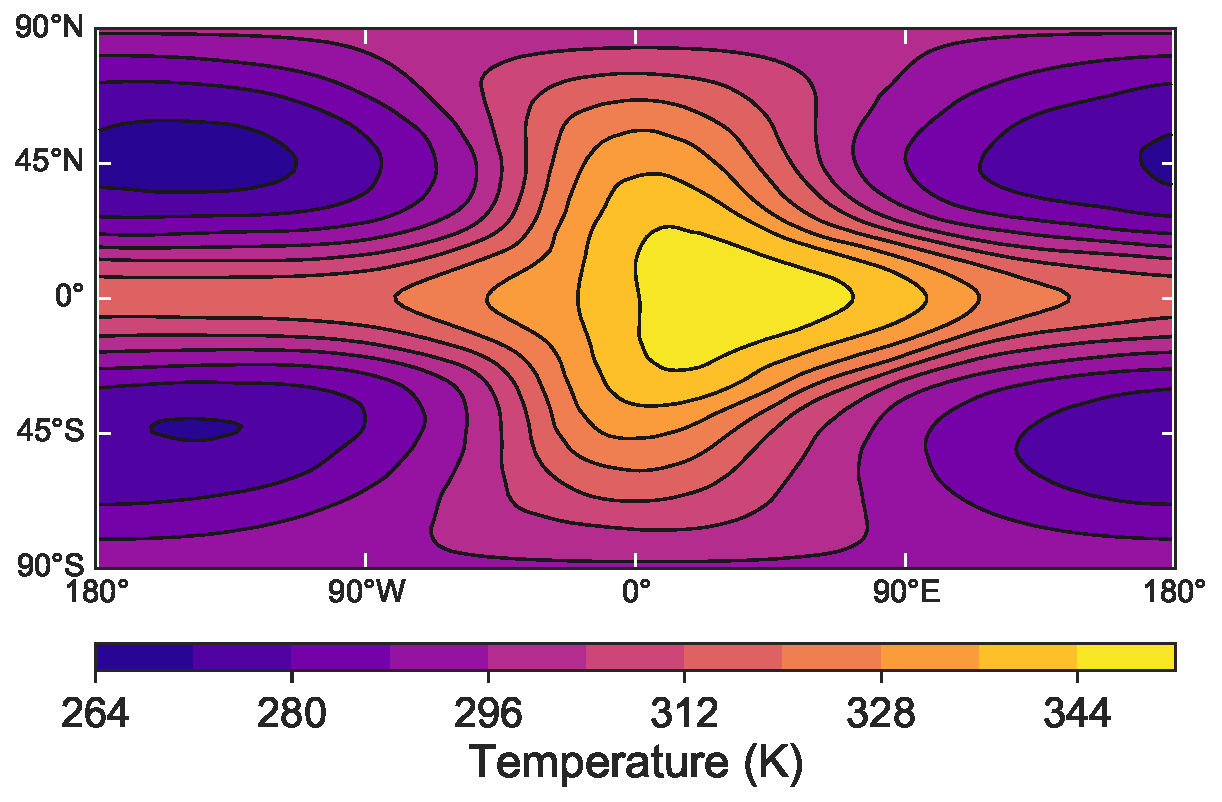
\includegraphics[width=\textwidth]{figures/wave-mean-flow/ar_mediumT_2day.pdf}
        \caption{\SI{1376}{\watt\per\metre\squared}, 2 days.}
        \label{fig:spherical-low-omega}
      \end{subfigure}
      \begin{subfigure}[b]{0.32\textwidth}
        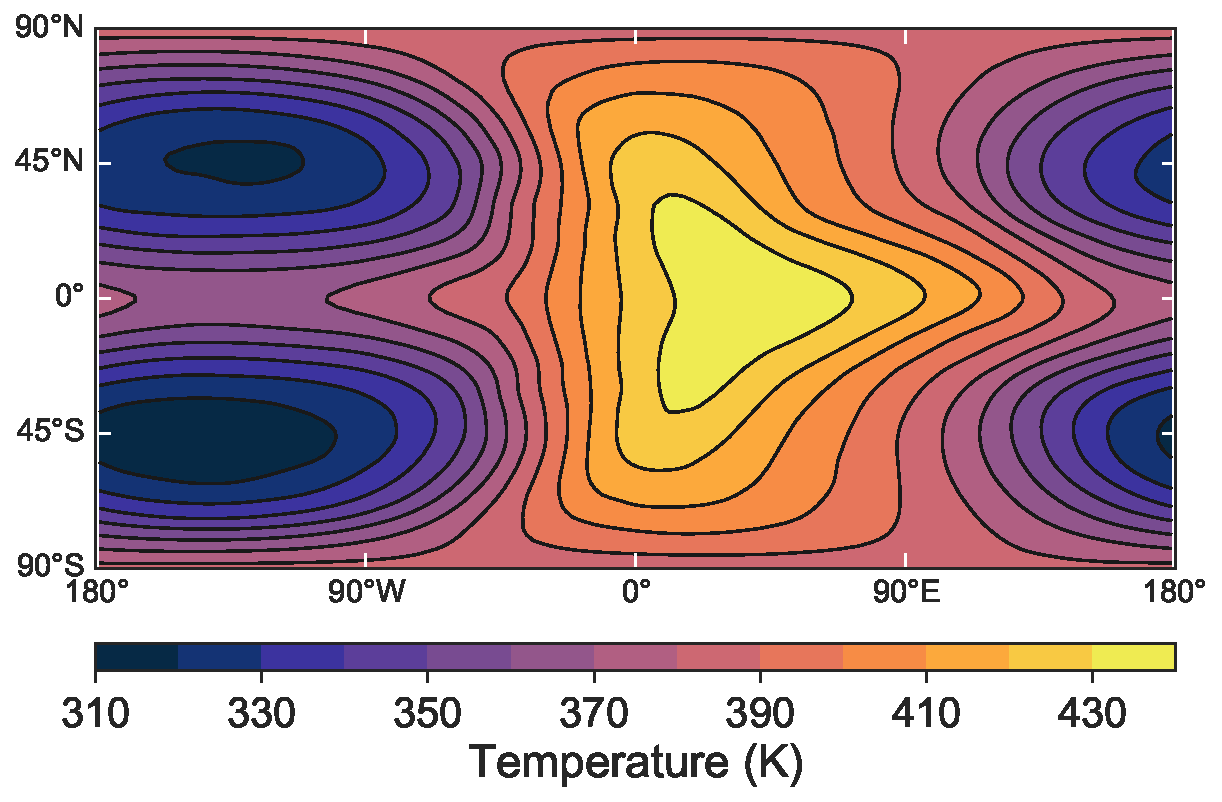
\includegraphics[width=\textwidth]{figures/wave-mean-flow/ar_highT_2day.pdf}
        \caption{\SI{4320}{\watt\per\metre\squared}, 2 days.}
        \label{fig:spherical-high-omega}
        \end{subfigure}
  \caption{The temperature at the \SI{500}{\milli\bar} level from a suite of simulations of tidally locked planets with 1 bar atmospheres in the GCM Exo-FMS, with different stellar constants and rotation periods. All other parameters are the same as those in Figure \ref{fig:example-gcm-results}. Reproduced with data from \citet{pierrehumbert2018review}.}
  \label{fig:gcm-suite-temperature}
\end{figure}



%SECTION CONCLUSIONS

%%%%%%%%%%%%%%%%%%%%%%%%%%%%%%%%%%%%
%DISCUSSION
\section{Discussion}\label{sec:shift-mechanism}

%  %SUBSECTION -- WAVES V ADVECTION
% \subsection{Hot-Spot Shift Mechanism}

Section \ref{sec:1d-scaling} showed how the hot-spot shift can be interpreted either as caused by advection of heat by the equatorial jet, or caused by a Doppler-shift of the stationary waves excited by the day-night forcing. These mechanisms are similar on some level, giving the same scaling behaviour on the equator as shown previously. However, they are physically different ideas and should have different effects. If advection by the jet produces the shift then the temperature and tracer fields in GCM simulations should be closely coupled. But, if the temperature field is instead set by the stationary wave pattern, it could be different to the distribution of tracers advected by the flow. Comparing temperature distributions to cloud distributions via thermal and optical phase curves could help distinguish these mechanisms.

This chapter suggests that the Doppler-shift of the waves is the appropriate mechanism, as it explains the global temperature and velocity distribution of the GCM simulations. Figure \ref{fig:eddy-gcm-results} shows eddy fields (i.e. with the zonal mean subtracted at every latitude) from the GCM simulation of a tidally locked planet shown in Figure \ref{fig:example-gcm-results}. This preserves the dominant wave-1 component forced by the day-night heating. Comparing Figure \ref{fig:eddy-gcm-results} with Figure \ref{fig:first-order-solutions} or Figure \ref{fig:spherical-solutions} shows how the wave solutions match the GCM results. The cold, anticlockwise Rossby waves are shifted to \ang{-90} in the GCM, matching the shifted pattern in Figure \ref{fig:expl-shifted-matsuno} rather than the non-shifted pattern in Figure \ref{fig:expl-non-shifted-matsuno}. The wave-based mechanism also explains the weak zonal flow east of the substellar point in the GCM simulation in Figure \ref{fig:example-gcm-results} --  the mean eastward zonal jet cancels with the local westward flow due to the waves shown in Figure \ref{fig:eddy-gcm-results}

This Doppler-shift mechanism was first put forward for tidally locked planets by \citet{tsai2014three}, for a zonally uniform flow. This chapter generalised the mechanism to the case of a zonally varying flow and an associated height perturbation, which was needed to fully match the global circulation in the GCM simulations. Advection of heat by the jet will still have some effect on the circulation, but the wave-based picture matches the circulation well enough that any advection effects appear to be minor. I have compared the shallow model to GCM simulations of a particular idealised planetary atmosphere, but very similar flow and wave patterns are seen in other studies of a variety of planets  \citep{charnay20153d, heng2015review, kataria2014atmospheric, mayne2017hotjupiter, boutle2017proxima}.

A compelling result of studying GFD on exoplanets is the possibility of plotting trends in atmospheric behaviour for classes of similar planets, as this is not possible with the individual data points of disparate Solar System planets. \citet{komacek2017daynightII} showed that the fractional day-night contrast $A = (T_{day}-T_{night})/T_{day}$ of many observed hot Jupiters increases with planetary equilibrium temperature. This is consistent with the discussion in Section \ref{sec:2d-scaling}, which shows in Figure \ref{fig:spherical-F-effect} how increased forcing gives a stronger wave-1 response than the wave-0 jet height field, giving a larger day-night contrast.

 \citet{komacek2017daynightII} also showed that the hot-spot shift on hot Jupiters decreases with increasing equilibrium temperature. This is consistent with Section \ref{sec:2d-scaling}, which predicted a decreased hot-spot shift at higher temperatures due to increased radiative damping. It is also consistent with the GCM simulations in Figure \ref{fig:gcm-suite-temperature}, where the tests with higher temperature had smaller hot-spot shifts. \citet{komacek2017daynightII} explained this trend as an increased damping rate giving a smaller shift as it dominates the heat transport via advection. This chapter instead explains the trend as due to the increased damping moving the stationary wave response into phase with the forcing, due to Equation \ref{eqn:am-U0}. As the number and quality of these observations increase, it will become possible to test the predictions of different descriptions of global circulation, such as the advection-based versus wave-based mechanisms discussed here.



\begin{figure}
  \centering
  \begin{subfigure}[b]{0.47\textwidth}
    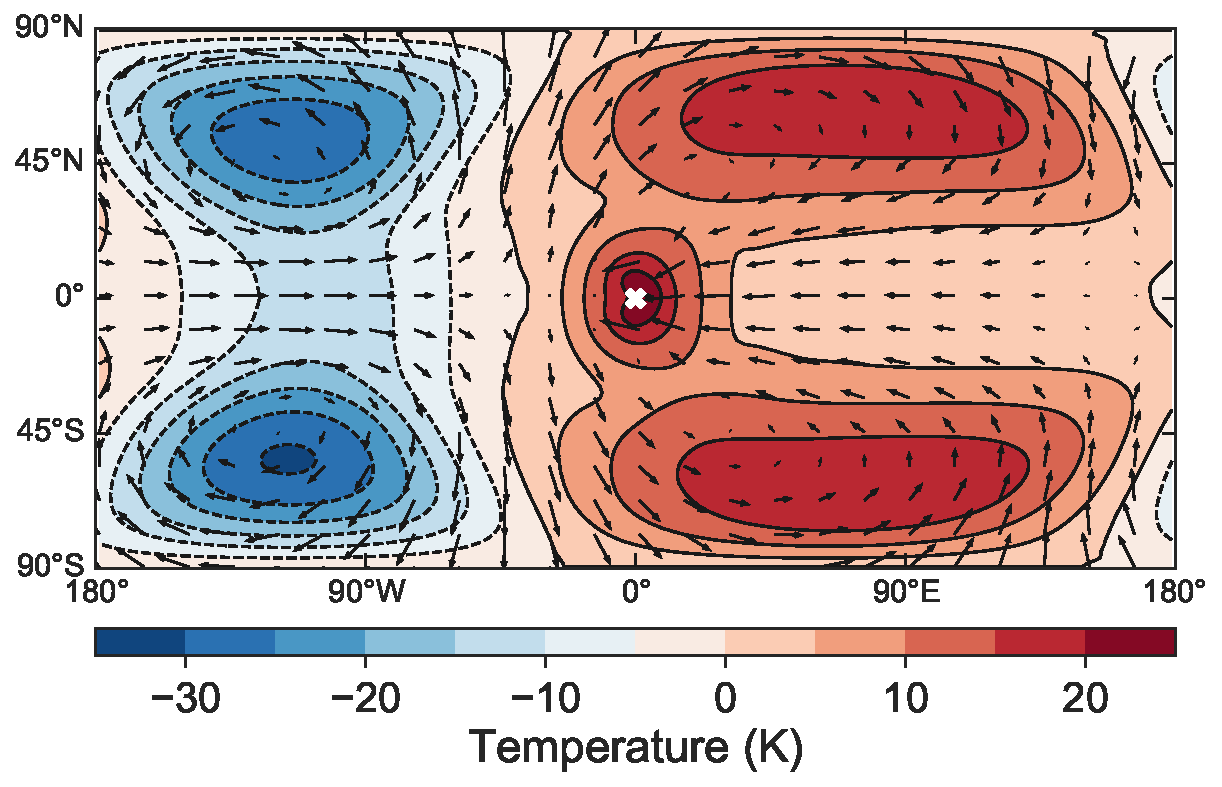
\includegraphics[width=\textwidth]{figures/wave-mean-flow/decomp-temp-10day-12.pdf}
    \caption{Eddy temperature and velocities.}
    \label{fig:spherical-low-omega}
  \end{subfigure}
  \quad
  \begin{subfigure}[b]{0.47\textwidth}
    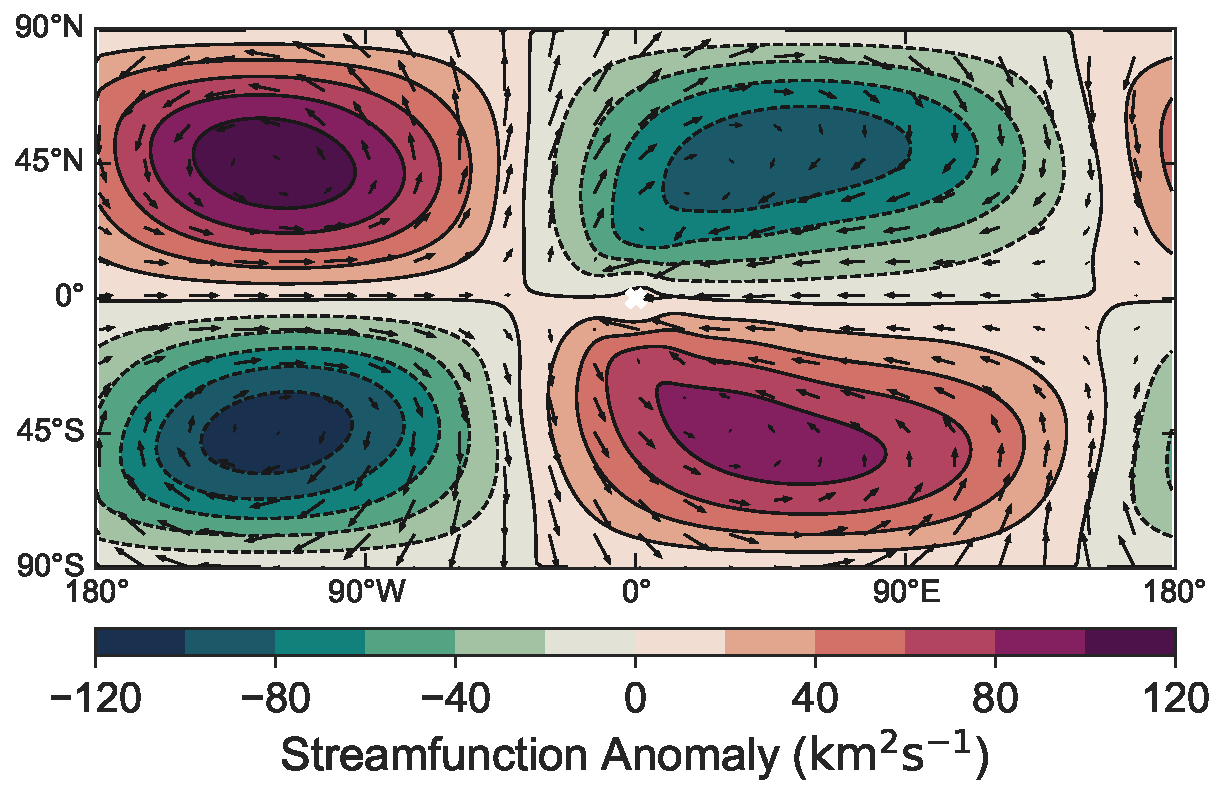
\includegraphics[width=\textwidth]{figures/wave-mean-flow/decomp-sf-10day-12.pdf}
    \caption{Eddy streamfunction and velocities.}
    \label{fig:spherical-low-omega}
  \end{subfigure}
\caption{The time-mean eddy temperature, velocity, and streamfunction fields (where the zonal mean at that latitude is subtracted from each point) on the half-surface pressure level of the GCM simulation shown in Figure \ref{fig:example-gcm-results}. These plots match the ``eddy'' shallow-water response in Figure \ref{fig:first-order-solutions}, before the zonally uniform jet is added.}\label{fig:eddy-gcm-results}
\end{figure}
%
% %SUBSECTION -- Comparing Prediction to Observations
% \subsection{Comparing Predictions to Observations}\label{sec:compare-obs}
%
% A compelling result of studying GFD on exoplanets is the possbility of plotting trends in atmospheric behaviour for classes of planet, in a way that is not possible with the individual data points of disparate Solar System planets. This makes it possible to test scaling relations such as those in this chapter, or in studies such as \citet{komacek2017daynightII} and \citet{zhang2017dynamics}. In this section, I compare the scaling relations from the linear shallow-water model in Section \ref{sec:sw-scaling-relations} to observed trends in day-night contrast and hot-spot shift for hot Jupiters with different equilibrium temperatures.
%
% Figure \ref{fig:komacek-obs-dnc} shows that the fractional day-night contrast $A = (T_{day}-T_{night})/T_{day}$ increases with planetary equilibrium temperature. This is consistent with the discussion in Section \ref{sec:2d-scaling}, which shows in Figure \ref{fig:spherical-F-effect} how increased forcing gives a stronger wave-1 response than the wave-0 jet height field, giving a larger day-night contrast. The damping rate will also increase at higher temperatures, which is predicted by Figure \ref{fig:spherical-damp-effect} to decrease the day-night contrast, but this effect appears to be weaker than the effect of the forcing. The observations are also consistent with the scaling behaviour of the GCM simulations in Figure \ref{fig:gcm-suite-temperature}, where increased forcing gives an increased day-night contrast. \citet{komacek2017daynightII} explained this trend with a balance of radiative versus advective timescales, using a different mechanism to the wave-based approach in this chapter, as discussed in the previous section.
%
% Figure \ref{fig:komacek-obs-hss} shows an observed decrease in hot-spot shift with increasing equilibrum temperature. This is consistent with Section \ref{sec:2d-scaling}, which predicts no effect on hot-spot shift from increased forcing, but a decreased hot-spot shift at higher temperatures due to increased radiative damping. It is also consistent with the GCM simulations in Figure \ref{fig:gcm-suite-temperature}, where the tests with higher temperature had smaller hot-spot shifts. \citet{komacek2017daynightII} explained this trend as an increased damping rate giving a smaller shift as it dominates the heat transport via advection. This chapter instead explains the trend as due to the increased damping moving the stationary wave response into phase with the forcing, due to Equation \ref{eqn:am-U0}.
%
% As the number and quality of these observations increase, it will become possible to test theories of global circulation in more detaill. The richness of possible behaviour due to variations in the atmospheric dynamics alone makes them vital to understand. Many mechanisms such as cloud formation, recombination of molecules, and magnetic effects have been invoked to explain observations of these planets. While this will be important in many cases, I suggest that much of the scaling behaviour will be explained by the variabile dynamical behaviour of the atmospheres.
%
% \begin{figure}
%   \centering
%   \begin{subfigure}[b]{0.45\textwidth}
%     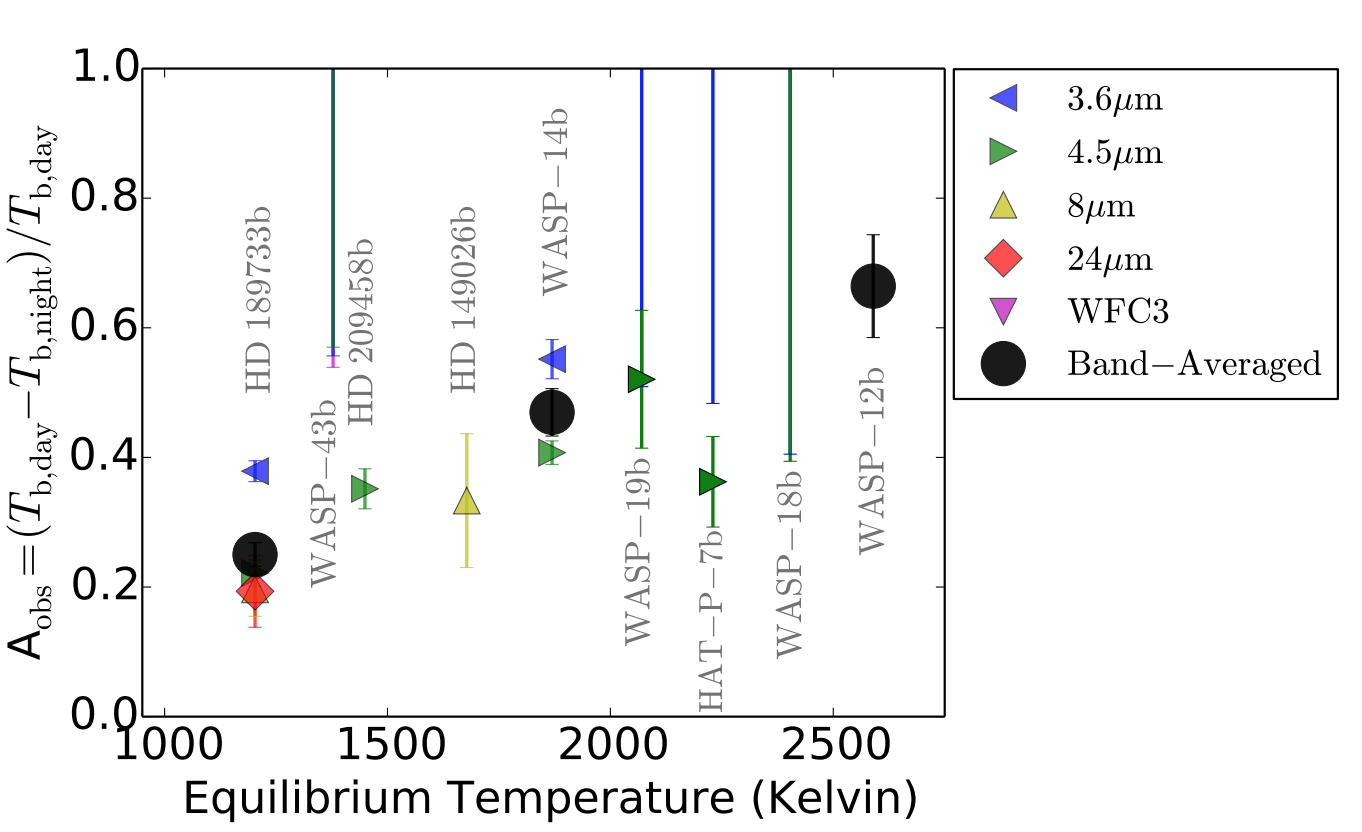
\includegraphics[width=\textwidth]{figures/wave-mean-flow/komacek-obs-dnc.png}
%     \caption{Observed day-night contrast versus planetary equilibrium temperature.}
%     \label{fig:komacek-obs-dnc}
%   \end{subfigure}
%   \begin{subfigure}[b]{0.45\textwidth}
%     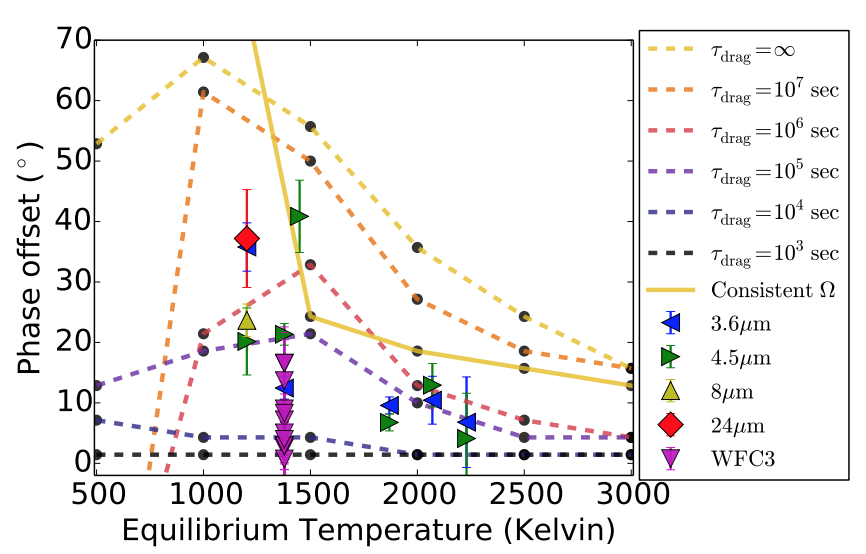
\includegraphics[width=\textwidth]{figures/wave-mean-flow/komacek-obs-hss.png}
%     \caption{Observed hot-spot shift versus planetary equilibrium temperature.}
%     \label{fig:komacek-obs-hss}
%   \end{subfigure}
% \caption{Observed day-night contrast and hot-spot shift versus planetary equilibrium temperature showing an increased contrast and decreased shift at higher temperatures, from \citet{komacek2017daynightII}.}\label{fig:komacek-obs}
% \end{figure}

% TO DO!
% %SUBSECTION --
% \subsection{Combining with Zonal Flow Theory}
%
% %SUBSECTION -- GCM SCALING
% \subsection{Observational Scaling Relations}
%
% The aim of these models is to explain the observed features of the circulation of tidally locked planets, in particular the hot-spot shift and day-night contrast.
%
% Figure X, after Figure X in \citet{komacek2017daynightII}, shows how the day-night contrast on tidally locked planets depends on equilibrium temperature.
%
% \citet{komacek2017daynightII} explained this trend with a decreasing radiative timescale. This chapter suggests an increased damping and stronger wave-1 response.
%
% Increasing hot-spot shift with temperature due to increased forcing?
%
% GCM prediction of scaling?
%
% \begin{table}[]
% \begin{tabular}{lllll}
% Planet & Wavelength & Hot-spot shift & Day-night contrast & Reference \\
% HD     & 1          & 40             & 0.5                & cite      \\
% H      &            &                &                    &           \\
%        &            &                &                    &           \\
%        &            &                &                    &           \\
%        &            &                &                    &           \\
%        &            &                &                    &           \\
%        &            &                &                    &           \\
%        &            &                &                    &           \\
%        &            &                &                    &
% \end{tabular}
% \end{table}


%%%%%%%%%%%%%%%%%%%%%%%%%%%%%%%%%%%%
%CONCLUSION
\section{Conclusions}

This chapter showed how the zonal flow discussed in Chapter \ref{ch:eqm-zonal-flow} produces the hot-spot shift and global circulation pattern of the atmospheres of tidally locked planets. I used a shallow-water model linearised about an equatorial jet $\overline{U}(y)$ to show how the flow Doppler-shifts the stationary waves excited by the day-night forcing. These waves combine with the zonally uniform jet to give the distinctive circulation pattern produced by GCM simulations.

Varying the parameters of the shallow-water model showed how the global circulation and temperature distribution scales with planetary parameters. This predicted scaling relations for observables such as day-night temperature contrast increasing with temperature, and hot-spot shift decreasing with temperature. These predictions are similar to the advection-based scaling of \citet{komacek2017daynightII} and \citet{zhang2017dynamics}, but have a different physical mechanism. I suggest that the wave-based mechanism is a better description of the global circulation and hot spot shift than the advection-based mechanism. Further observations could test the predictions of these mechanisms to find which is a better model.

The next step will be to the linear model to predict the equilibrium flow speeds and global temperature fields of tidally locked planets. The model could also be used to find the free modes in their atmospheres, then to compare these to the travelling waves and instabilities seen in simulations and observations \citep{pierrehumbert2018review, armstrong2017variability}.

This chapter showed how the interaction between the equatorial jet and the stationary waves excited by the instellation produces the global circulation and temperature distribution in the atmosphere of a tidally locked planet. The rest of this thesis will apply this theory to a case study of the planet 55 Cancri e, comparing simple models and numerical simulations to observations of its temperature distribution.

% We calculated the free modes of the beta-plane model in a shear flow, and found some unstable modes when the shear was strong enough, which could correspond to this variability.


%RESTATE SECTION CONCLUSIONS

%OPEN OUT CONCLUSIONS



% \bibliographystyle{unsrtnat}
% \bibliography{../references.bib}
